\chapter{Proposed Models}
\pagestyle{default}
\thispagestyle{default}

This chapter presents the proposed end-to-end solution developed for the automated detection of chest diseases and bone fractures from medical imaging data. The chapter aims to provide a comprehensive description of the overall system architecture as well as a detailed explanation of the individual models that constitute the proposed solution.

The chapter begins by outlining the solution architecture, which describes the complete pipelines of the system, including the high-level data flow and processing in the DL pipeline, and the backend processes and structure. This section illustrates how both the DL pipeline and the system's backend operate cohesively to form a unified diagnostic framework.

Subsequently, the chapter discusses the transfer learning models used in the proposed system. This section explains the pre-trained architectures employed, and their advantages in medical image analysis.

The medical image routing model is then introduced, which serves as an intelligent intermediary responsible for directing input images to the appropriate diagnostic model based on anatomical or modality-specific characteristics. This component plays a critical role in enabling the downstream models to act on an expected input image modality and anatomical region, it is also crucial in dropping out-of-distribution input data from being processed by the diagnostic models.

Following this, the bone fracture detection model is presented in detail. This section describes the model architecture, and classification approach used to identify bone fractures from radiographic images.

Then, an in-depth explanation of the chest disease detection model, which focuses on identifying various thoracic conditions from chest X-ray images, is presented. The section covers the model design, feature extraction process, and classification methodology employed to achieve robust disease detection.

Finally, the chapter ends with a summary to conclude all the information presented and an emphasis is put on the key information given in the chapter.

\section{Proposed Architecture}
\label{sec:solution_architecture}

This chapter presents the architecture of the proposed intelligent medical image analysis framework. The system is designed as a hierarchical, modality-aware diagnostic pipeline capable of analyzing heterogeneous medical imaging data while maintaining high levels of reliability, interpretability, and scalability. The architecture addresses a practical challenge frequently encountered in real-world clinical environments: different diseases are diagnosed using different imaging modalities, and therefore a single monolithic model may not be the most effective solution. Instead, the proposed framework decomposes the overall diagnostic task into a sequence of specialized stages that collectively form an end-to-end decision-making pipeline.

The framework has been designed to support the automated analysis of chest radiographs and computed tomography (CT) scans. More specifically, the system is capable of detecting COVID-19, Tuberculosis, and Pneumonia from chest X-ray images, while also performing lung cancer detection from CT scans. In addition to disease classification, the framework incorporates Explainable Artificial Intelligence (XAI) mechanisms to improve transparency and trustworthiness, as well as Federated Learning (FL) capabilities to facilitate privacy-preserving collaborative model development across multiple healthcare institutions.

The overall architecture follows a two-level classification paradigm. At the first level, an intelligent routing model determines the modality of the incoming image and verifies whether it belongs to one of the supported image categories. At the second level, modality-specific diagnostic models perform disease prediction. This hierarchical structure enables the system to leverage specialized classifiers that are optimized for their respective tasks while reducing the complexity associated with training a single generalized model.

Figure~\ref{fig:full_overall_architecture} presents a high-level overview of the proposed framework.

\begin{figure}[H]
	\centering
	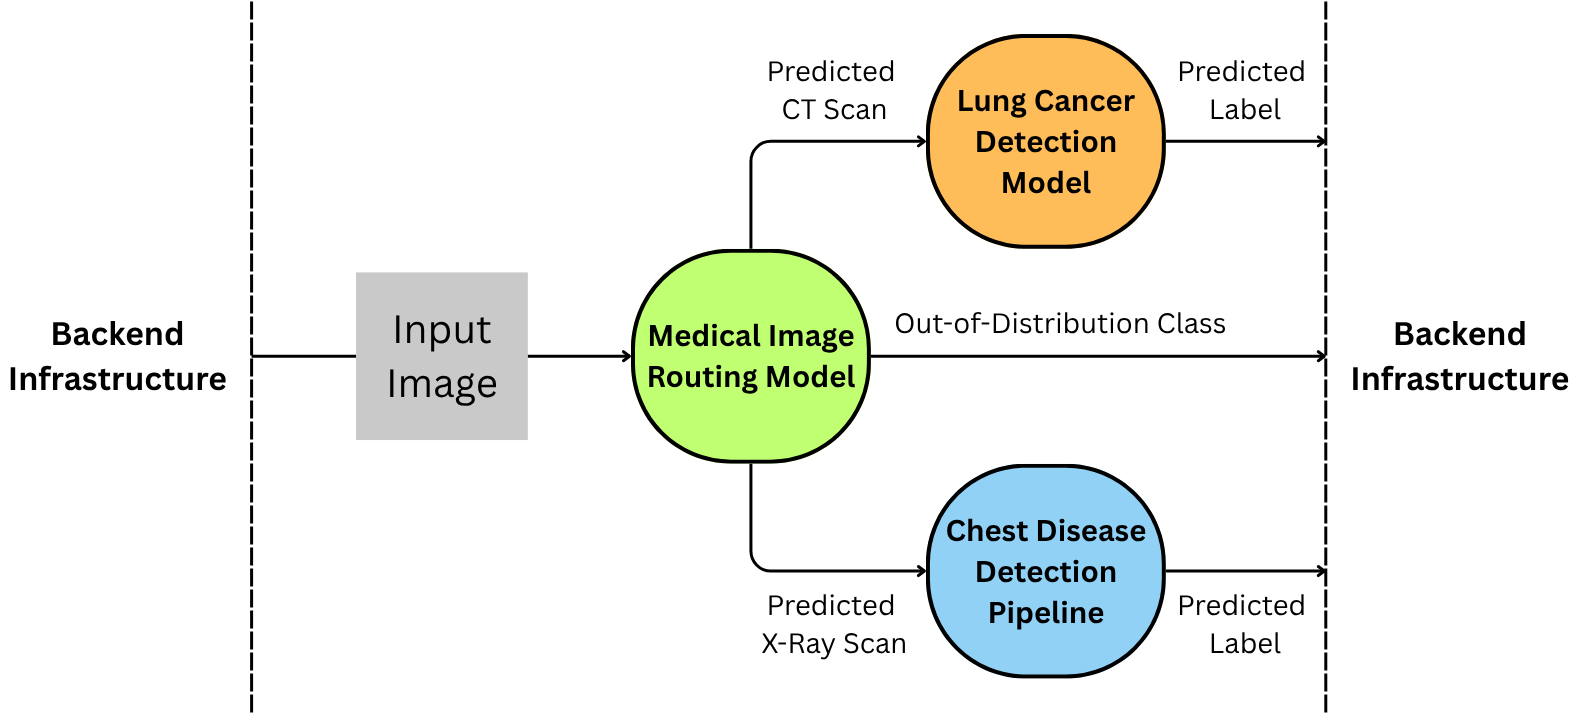
\includegraphics[width=\linewidth]{assets/full_project_arch.png}
	\caption{High-level architecture of the proposed framework. The system consists of a modality routing model, specialized disease classifiers, Explainable AI modules, and a Federated Learning infrastructure connecting multiple healthcare institutions.}
	\label{fig:full_overall_architecture}
\end{figure}

\subsection{Architectural Design Philosophy}

The proposed framework was developed according to several architectural principles that were established at the beginning of the system design process. These principles were intended to ensure that the resulting framework would not only achieve strong predictive performance but would also remain practical for real-world deployment in healthcare environments.

One of the most important design considerations was modality awareness. Medical images generated by different imaging technologies exhibit fundamentally different visual characteristics and diagnostic properties. Chest radiographs provide projection-based representations of thoracic structures, whereas CT scans generate detailed cross-sectional views that reveal significantly more anatomical information. These differences influence the types of features that neural networks must learn in order to perform accurate diagnosis. A single generalized model trained across multiple modalities may struggle to simultaneously learn optimal representations for all imaging types. Consequently, the proposed architecture explicitly separates modality identification from disease diagnosis. This design allows each diagnostic model to focus exclusively on data originating from the modality for which it was designed.

Another fundamental design principle was task specialization. The diseases targeted by this work differ substantially in terms of pathological manifestations, imaging characteristics, and diagnostic requirements. COVID-19, Tuberculosis, and Pneumonia are primarily identified using chest radiographs, whereas lung cancer diagnosis often relies on the higher anatomical resolution available in CT imaging. Rather than attempting to train a single network to recognize all diseases across all modalities, the proposed framework distributes these tasks among specialized models. This decomposition reduces task complexity and allows each model to learn more discriminative feature representations relevant to its specific diagnostic objective.

Reliability and patient safety also played a significant role in the architectural design. Medical AI systems must operate in environments where unexpected inputs are inevitable. Hospital information systems frequently contain diverse imaging studies, and a deployed diagnostic model may encounter unsupported image types, corrupted files, incomplete scans, or non-medical images. If such inputs are processed without validation, the resulting predictions may be unreliable and potentially dangerous. To address this issue, the proposed framework incorporates an explicit out-of-distribution detection mechanism within the routing stage. This component enables the system to identify unsupported inputs before they reach the diagnostic models.

Transparency represents another critical requirement for healthcare AI systems. Clinical practitioners often require evidence supporting automated predictions before integrating them into their decision-making processes. While deep neural networks have demonstrated remarkable predictive capabilities, they are frequently criticized for their lack of interpretability. The proposed architecture therefore integrates explainability mechanisms directly into the diagnostic workflow. These mechanisms provide visual explanations that highlight image regions contributing to the final prediction, thereby allowing clinicians to better understand and validate the reasoning process of the model.

Finally, the architecture was designed with scalability and long-term deployment in mind. Healthcare institutions are often unable to share patient data due to privacy regulations, legal restrictions, and ethical concerns. Consequently, the framework incorporates Federated Learning capabilities that enable multiple institutions to collaboratively improve model performance without exchanging raw patient information. This design promotes the creation of a continuously improving diagnostic ecosystem while preserving patient confidentiality.

\subsection{System Workflow}

The complete workflow of the proposed framework begins when a medical image is submitted to the system. Following acquisition, the image undergoes preprocessing operations intended to standardize the input format and improve compatibility with the downstream neural networks. These operations may include resizing, normalization, intensity standardization, and other transformations required by the underlying deep learning models.

Once preprocessing is completed, the image is forwarded to the first level of the architecture, namely the modality routing model. The purpose of this stage is to determine the nature of the input image and identify the appropriate diagnostic pathway. The routing decision governs all subsequent processing stages and therefore serves as a critical component of the framework.

After the routing decision is generated, the image is directed toward a specialized diagnostic model. Images identified as chest radiographs are analyzed by the chest disease classifier, while CT scans are analyzed by the lung cancer detection model. Images identified as out-of-distribution are excluded from automated diagnosis and may instead be flagged for manual review by healthcare personnel.

Following disease prediction, explainability modules generate visual interpretations of the model output. These interpretations provide insight into the image regions that most strongly influenced the prediction process. Finally, the prediction and associated explanation are presented to the clinician. During model training, Federated Learning mechanisms facilitate collaborative model improvement across multiple participating institutions.

Figure~\ref{fig:classification_tree} illustrates the classification pathway implemented by the proposed framework.

\begin{figure}[H]
	\centering
	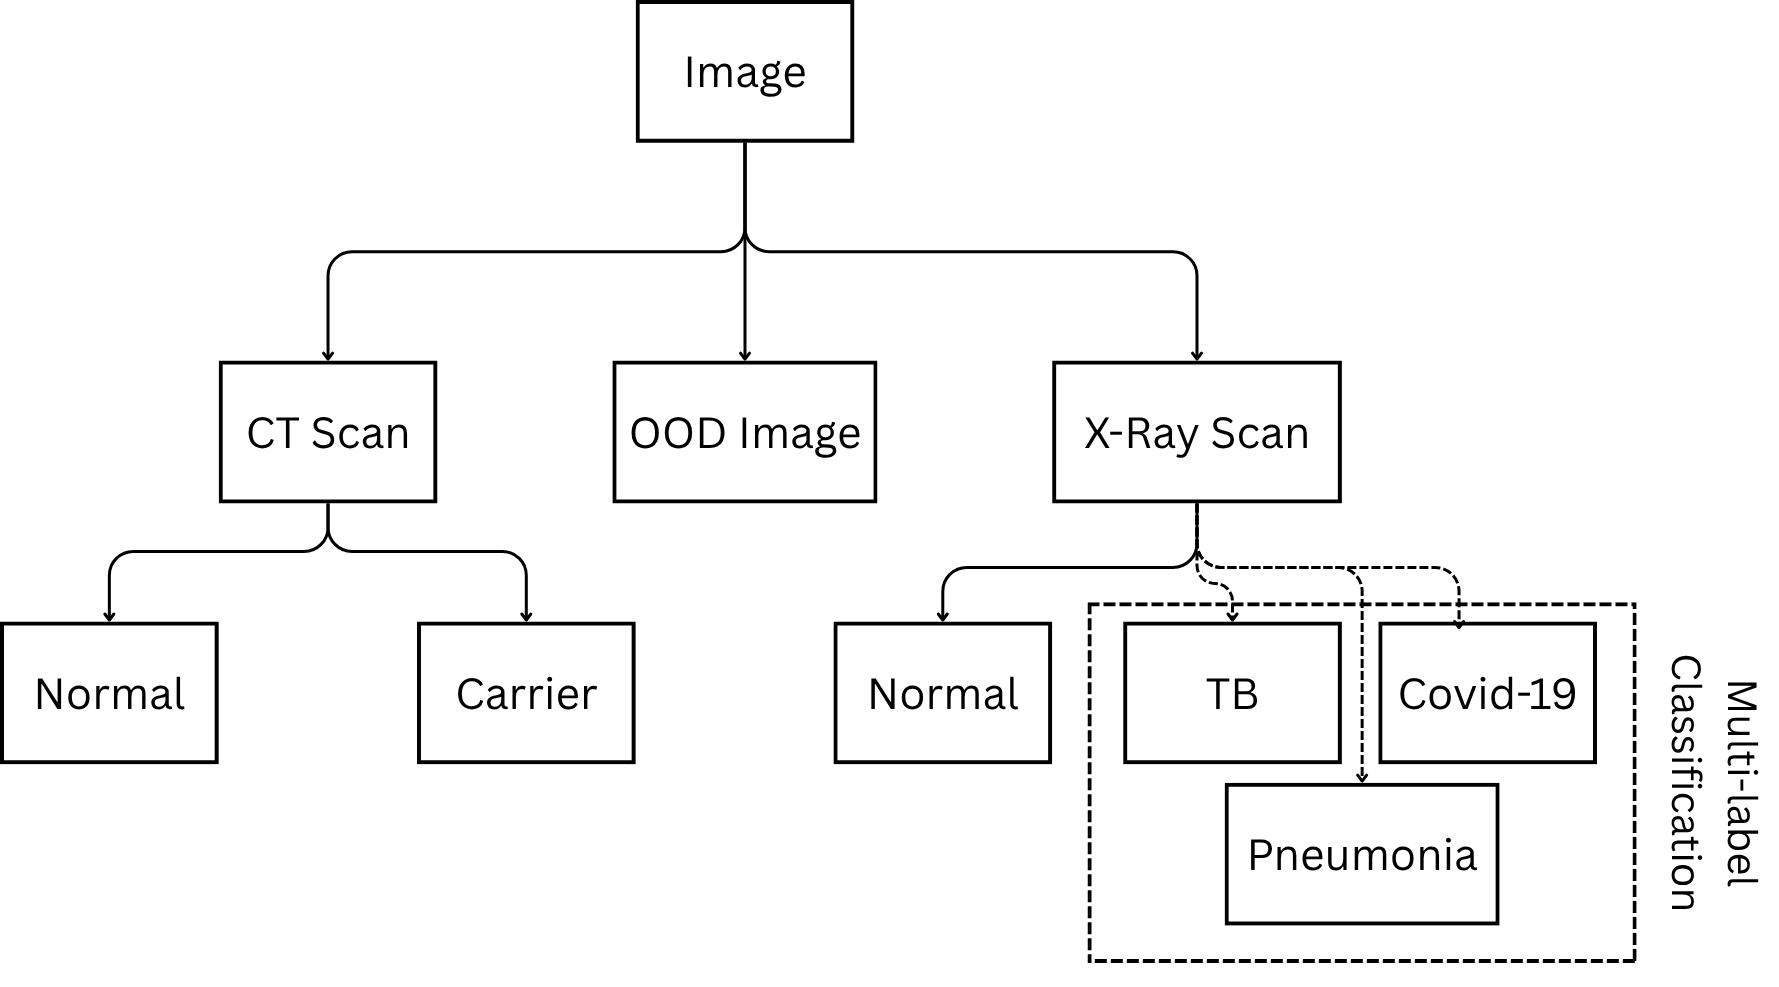
\includegraphics[width=0.8\linewidth]{assets/classification_tree.png}
	\caption{Classification tree of the proposed two-level framework. The routing model first determines the image modality before directing the image toward the appropriate disease-specific classifier.}
	\label{fig:classification_tree}
\end{figure}

\subsection{Level One: Modality Routing and Out-of-Distribution Detection}

The first level of the proposed architecture functions as an intelligent routing mechanism responsible for identifying the modality of the incoming image. Although this component performs a relatively simple classification task compared to disease diagnosis, its importance should not be underestimated. Every subsequent prediction generated by the framework depends directly on the correctness of the routing decision.

Formally, let $I$ denote an input image. The routing model $R(\cdot)$ maps the image into one of three categories:

\begin{equation}
	R(I) \in \{\text{X-ray}, \text{CT}, \text{OOD}\}
\end{equation}

where OOD represents an out-of-distribution image.

The motivation for introducing a dedicated routing stage arises from the substantial differences between X-ray and CT imaging modalities. Chest radiographs represent two-dimensional projection images that summarize anatomical information along a viewing direction. In contrast, CT scans provide detailed cross-sectional information that enables the visualization of internal structures with considerably greater precision. These differences imply that the features required for effective diagnosis are modality-dependent. Routing images to specialized models therefore allows the framework to exploit modality-specific representations rather than relying on a generalized feature extraction strategy.

From a computational perspective, routing also improves efficiency. Without this stage, every image would need to be processed by every available diagnostic model, resulting in increased computational cost and unnecessary inference overhead. By ensuring that each image is evaluated only by the most relevant classifier, the routing model reduces resource consumption and improves scalability.

An equally important function of the routing stage is out-of-distribution detection. In practical deployment scenarios, healthcare systems may receive images that differ significantly from those used during training. Examples include magnetic resonance imaging studies, ultrasound images, pathology slides, non-medical photographs, or improperly formatted files. Diagnostic models are generally incapable of producing reliable predictions for such inputs because they fall outside the distribution of the training data.

To mitigate this problem, the routing model incorporates a dedicated OOD category. Images assigned to this category are prevented from entering the diagnostic pipeline. This safeguard reduces the likelihood of erroneous predictions and contributes to the overall reliability of the framework. From a clinical perspective, this mechanism functions as a preliminary quality-control layer that ensures only supported image types proceed to automated analysis.

\subsection{Level Two: Chest Disease Detection Model}

Images identified as chest radiographs are forwarded to the chest disease classification model. This model is responsible for detecting three clinically significant respiratory diseases: COVID-19, Tuberculosis, and Pneumonia.

The selection of these diseases was motivated by both clinical relevance and public health importance. COVID-19 remains one of the most extensively studied respiratory illnesses in recent years and has highlighted the importance of rapid imaging-based screening techniques. Tuberculosis continues to represent a major global health challenge, particularly in developing countries where early detection plays a crucial role in disease management and transmission control. Pneumonia remains one of the most common respiratory infections worldwide and is associated with substantial morbidity and mortality across multiple age groups.

A key characteristic of the proposed chest disease model is its formulation as a multi-label classification problem rather than a conventional multi-class classification problem. This distinction is essential because the targeted diseases are not mutually exclusive. In clinical practice, a patient may simultaneously exhibit radiological findings associated with multiple respiratory conditions. For example, viral infections may be accompanied by secondary bacterial pneumonia, and complex pathological interactions may lead to overlapping imaging manifestations.

Traditional multi-class classification assumes that each sample belongs to exactly one category. Such an assumption would force the model to select a single disease label even when multiple diseases are present. This formulation would therefore fail to accurately represent many real-world clinical scenarios.

To address this limitation, the proposed architecture employs independent disease predictions. Let

\begin{equation}
	\mathbf{y} =
	[y_{\text{COVID}}, y_{\text{TB}}, y_{\text{Pneumonia}}]
\end{equation}

denote the output vector generated by the classifier. Each element corresponds to the estimated probability that a specific disease is present within the image.

Unlike a softmax-based multi-class architecture, the output layer uses independent sigmoid activations. This allows the model to assign high probabilities to multiple diseases simultaneously whenever appropriate. The final prediction for each disease is obtained by applying a predefined threshold:

\begin{equation}
	\hat{y}_i=
	\begin{cases}
		1 & y_i \geq \tau \\
		0 & y_i < \tau
	\end{cases}
\end{equation}

where $\tau$ denotes the classification threshold.

This formulation better reflects the realities of clinical diagnosis and provides greater flexibility when interpreting model outputs. Instead of receiving a single categorical prediction, clinicians are presented with independent disease probabilities that can be incorporated into broader diagnostic assessments.

\subsection{Level Two: Lung Cancer Detection Model}

Images classified as CT scans are forwarded to the lung cancer detection model. The decision to utilize CT imaging for lung cancer analysis is motivated by the superior anatomical detail provided by computed tomography compared to conventional radiography.

Lung cancer frequently manifests through subtle structural abnormalities such as pulmonary nodules, irregular masses, and localized tissue changes that may not be visible in chest radiographs. The high spatial resolution of CT imaging enables these features to be observed with significantly greater clarity, making CT the preferred modality for many lung cancer screening and diagnostic procedures.

The objective of the lung cancer model is to determine whether cancer-related findings are present within the input scan. The classifier can be represented mathematically as

\begin{equation}
	P_{\text{Cancer}} = C(I)
\end{equation}

where $C(\cdot)$ denotes the lung cancer detection network and $P_{\text{Cancer}}$ represents the estimated probability of malignancy.

By focusing exclusively on CT-derived information, the model can dedicate its representational capacity to learning highly discriminative cancer-related features. This specialization improves the model's ability to identify subtle pathological patterns that may be difficult to detect using a generalized classifier.

\subsection{Explainable Artificial Intelligence Integration}

The increasing adoption of artificial intelligence within healthcare has generated significant interest in model interpretability. Although deep learning systems are capable of achieving remarkable predictive performance, their internal decision-making processes often remain difficult to understand. This lack of transparency can hinder clinical adoption, particularly when predictions influence critical healthcare decisions.

To address this challenge, Explainable Artificial Intelligence techniques are integrated directly into the proposed architecture. Rather than treating explainability as an optional post-processing step, it is considered a fundamental component of the diagnostic workflow.

Following prediction generation, the explainability module produces visual explanations illustrating the regions of the image that most strongly influenced the model's decision. These visualizations may take the form of saliency maps, activation maps, attention maps, or gradient-based explanations depending on the selected implementation.

The integration of explainability serves several purposes. First, it increases clinician confidence by providing visual evidence supporting the model's prediction. Second, it facilitates model validation by enabling researchers to verify that the network is focusing on medically meaningful regions rather than irrelevant artifacts. Third, it assists in identifying potential biases or failure modes that may otherwise remain hidden within the network. Ultimately, explainability strengthens the collaborative relationship between clinicians and AI systems by transforming predictions into interpretable decision-support information.

\subsection{Federated Learning Infrastructure}

A distinguishing feature of the proposed framework is its support for Federated Learning. This capability was incorporated to address one of the most significant challenges facing medical artificial intelligence: limited access to large and diverse datasets.

Traditional deep learning systems typically rely on centralized training approaches in which data from multiple institutions are collected and stored in a single repository. While effective from a machine learning perspective, this strategy introduces substantial privacy, security, and regulatory concerns. Healthcare organizations are often prohibited from sharing patient data due to legal and ethical restrictions.

Federated Learning offers an alternative paradigm in which training occurs locally at each institution. Rather than transmitting patient data, participating hospitals train local models using their own datasets and share only model parameters or parameter updates. These updates are subsequently aggregated to produce a global model.

Let $w_i$ denote the model parameters learned by institution $i$, and let $n_i$ denote the number of training samples available at that institution. Using the Federated Averaging algorithm, the global model is computed as

\begin{equation}
	w_{\text{global}}
	=
	\sum_{i=1}^{K}
	\frac{n_i}{\sum_{j=1}^{K}n_j}
	w_i
\end{equation}

where $K$ represents the total number of participating institutions.

Beyond privacy preservation, Federated Learning provides several additional benefits. Because participating institutions often serve different patient populations, the resulting datasets contain greater demographic, geographic, and clinical diversity. Training across such heterogeneous data sources can improve model generalization and reduce susceptibility to institution-specific biases. Furthermore, the collaborative nature of Federated Learning enables continuous improvement of the framework as new institutions join the network and contribute additional knowledge.


\section{Transfer-Learning Models Used}
This section presents the transfer learning models employed in the proposed system and discusses the rationale behind their selection. Transfer learning is adopted to leverage pre-trained deep neural networks that have been trained on large-scale datasets, enabling effective feature extraction and improved generalization in medical imaging tasks with limited labeled data. The section provides an overview of the selected architectures and highlights their suitability for different components of the proposed diagnostic pipeline.

\subsection{ResNet50 Model} \label{subsec:resnet50-arch}
Residual Networks (ResNets) were introduced to address the degradation problem observed in deep convolutional neural networks, where increasing network depth leads to saturation or decline in training accuracy. This issue emerges due to optimization difficulties such as vanishing gradients. ResNet addresses this limitation through the concept of residual learning, which allows the training of substantially deeper networks by enabling more effective gradient propagation.

The key idea of residual learning is to reformulate the learning objective of a neural network block. Instead of directly learning a desired underlying mapping \( H(x) \), a residual block learns a residual function \( F(x) \) such that:
\[
H(x) = F(x) + x
\]
where \( x \) represents the input to the residual block and \( F(x) \) represents the output of the stacked convolutional layers within the block. The identity shortcut connection that performs the addition allows gradients to flow directly through the network during backpropagation, thereby minimizing vanishing gradient effects and improving training stability.

\begin{figure}[h]
	\centering
	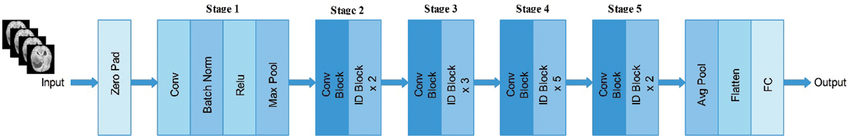
\includegraphics[width=\linewidth]{assets/resnet50.png}
	\caption{Architecture of the ResNet50 illustrating the successive stages of the model.}
	\label{fig:resnet50-arch}
\end{figure}

As illustrated in Figure~\ref{fig:resnet50-arch}, the ResNet50 architecture begins with an initial convolutional layer preceded by zero padding, followed by batch normalization, a ReLU activation function, and a max pooling operation. This initial stage is responsible for extracting low-level visual features from the input image. The network then proceeds through five sequential stages composed of convolutional blocks and identity blocks, each incorporating residual connections that bypass multiple convolutional layers.

ResNet50 employs a bottleneck design within its residual blocks, consisting of a sequence of \(1 \times 1\), \(3 \times 3\), and \(1 \times 1\) convolutional layers. The \(1 \times 1\) convolutions are used to reduce and subsequently restore feature dimensionality, thereby decreasing computational complexity while preserving representational power. This design enables ResNet50 to achieve substantial depth without incurring prohibitive computational costs.

Compared to shallower variants such as ResNet18 and ResNet34, ResNet50 offers increased representational capacity and improved ability to capture complex and abstract visual patterns. While deeper variants such as ResNet101 and ResNet152 further extend network depth, they introduce higher computational overhead and an increased risk of overfitting, particularly in medical imaging applications where annotated data is often limited. Consequently, ResNet50 represents a balanced trade-off between depth, efficiency, and performance within the ResNet family.

As shown in Figure~\ref{fig:resnet50-arch}, the final stages of ResNet50 consist of a global average pooling layer, followed by feature flattening and a fully connected layer. In transfer learning scenarios, this classification head can be replaced or fine-tuned to adapt the network to domain-specific medical tasks.

In the context of medical image analysis, ResNet50 is well-suited for extracting both low-level structural features and high-level semantic representations relevant to pathological patterns. The residual connections promote feature reuse and robust optimization, which is particularly important for detecting subtle abnormalities in medical images such as fractures or thoracic diseases. These characteristics make ResNet50 a reliable and widely adopted backbone for medical image classification tasks.

\subsection{DenseNet121 Model}
\label{subsec:densenet121}

DenseNet121 is a deep convolutional neural network architecture belonging to the family of Densely Connected Convolutional Networks (DenseNets), which were introduced by Huang \textit{et al.} in 2017 to address several limitations associated with traditional deep neural networks. DenseNet architectures were designed to improve feature propagation, encourage feature reuse, alleviate the vanishing gradient problem, and reduce the number of trainable parameters while maintaining high classification performance. Since its introduction, DenseNet121 has become one of the most widely adopted architectures in medical image analysis due to its ability to learn rich hierarchical representations from relatively limited datasets.

The fundamental idea behind DenseNet differs significantly from that of conventional convolutional neural networks. In traditional architectures, each layer receives information only from the immediately preceding layer and passes its output solely to the next layer. Although this sequential information flow is effective, it may lead to difficulties in gradient propagation as network depth increases. Furthermore, many learned feature maps become redundant because similar patterns are repeatedly relearned at different layers throughout the network.

To address these limitations, DenseNet introduces direct connections between layers. Instead of receiving input from only the previous layer, each layer receives the feature maps generated by all preceding layers within the same dense block. Consequently, information can flow directly from earlier layers to later layers without repeatedly passing through intermediate transformations. This dense connectivity pattern enables more efficient feature reuse and facilitates the training of very deep networks.

Figure~\ref{fig:densenet121_architecture} illustrates the overall architecture of DenseNet121.

\begin{figure}[H]
	\centering
	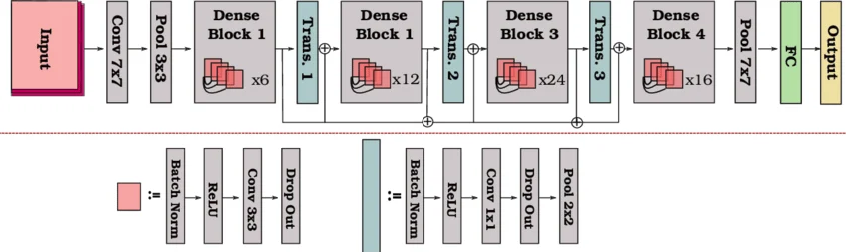
\includegraphics[width=\linewidth]{assets/DenseNet121.png}
	\caption{Overall architecture of DenseNet121 showing the arrangement of dense blocks, transition layers, and the final classification stage.}
	\label{fig:densenet121_architecture}
\end{figure}

\subsubsection{Motivation Behind Dense Connectivity}

As neural networks become deeper, the flow of information and gradients through the network becomes increasingly difficult. One of the most common challenges encountered in deep architectures is the vanishing gradient problem, where gradients become progressively smaller as they are propagated backward through many layers. When gradients become extremely small, early layers receive little useful learning signal, slowing convergence and potentially reducing overall performance.

Residual Networks (ResNets) partially addressed this issue through skip connections that allow gradients to bypass certain transformations. DenseNet extends this concept further by establishing direct connections between every pair of layers within a dense block. Instead of merely adding outputs from previous layers, DenseNet concatenates them. This strategy preserves information from all preceding layers and makes it directly accessible to subsequent layers.

The dense connectivity mechanism provides several important benefits. First, it improves gradient flow during training, allowing deeper networks to be optimized more effectively. Second, it encourages feature reuse, reducing redundancy among learned representations. Third, it improves parameter efficiency because layers can leverage previously learned features rather than learning entirely new representations from scratch.

\subsubsection{Dense Connectivity Mechanism}

The defining characteristic of DenseNet is the dense connection pattern between layers. Let $x_0$ represent the input to a dense block and let $x_l$ denote the output of the $l^{th}$ layer. Unlike traditional convolutional networks, where the output of layer $l$ depends only on the output of layer $l-1$, DenseNet computes each layer using the outputs of all preceding layers:

\begin{equation}
	x_l = H_l([x_0, x_1, x_2, ..., x_{l-1}])
\end{equation}

where:

\begin{itemize}
	\item $H_l(\cdot)$ denotes a composite transformation.
	\item $[\cdot]$ represents the concatenation operation.
	\item $x_0, x_1, ..., x_{l-1}$ are the feature maps generated by previous layers.
\end{itemize}

The concatenation operation differs fundamentally from the addition operation used in residual networks. Instead of merging features by summation, DenseNet preserves all previous feature maps and passes them directly to subsequent layers. As a result, each layer has access to both low-level and high-level information simultaneously.

This dense feature propagation mechanism allows later layers to exploit a richer collection of learned representations, improving feature diversity and reducing information loss.

\subsubsection{Dense Blocks}

The primary computational components of DenseNet121 are the dense blocks. A dense block consists of multiple densely connected layers arranged according to the connectivity pattern described previously.

Within each dense block, every layer receives as input the concatenated outputs of all preceding layers. Consequently, the number of feature maps grows progressively as additional layers are added. This growth is controlled through a parameter known as the \textit{growth rate}.

The growth rate, typically denoted by $k$, determines the number of new feature maps generated by each layer. If the input to a dense block contains $F_0$ feature maps and the block contains $L$ layers, the total number of feature maps at the end of the block can be expressed as:

\begin{equation}
	F = F_0 + kL
\end{equation}

where:

\begin{itemize}
	\item $F_0$ is the number of initial feature maps.
	\item $k$ is the growth rate.
	\item $L$ is the number of layers within the block.
\end{itemize}

For DenseNet121, the growth rate is typically set to 32. This means that each layer contributes 32 new feature maps while simultaneously utilizing all previously generated feature maps.

The use of a relatively small growth rate contributes to the parameter efficiency of DenseNet architectures, allowing them to achieve competitive performance with fewer parameters than many alternative architectures.

\subsubsection{Composite Function within Dense Layers}

Each layer within a dense block consists of a sequence of operations designed to transform incoming feature maps into more informative representations.

The composite transformation $H_l(\cdot)$ generally consists of:

\begin{enumerate}
	\item Batch Normalization (BN)
	\item Rectified Linear Unit (ReLU)
	\item Convolution
\end{enumerate}

This sequence is commonly referred to as the BN-ReLU-Conv pattern.

Batch normalization stabilizes the learning process by normalizing intermediate activations. This reduces internal covariate shift and allows higher learning rates to be used during training.

The ReLU activation function introduces non-linearity into the network and is defined as:

\begin{equation}
	f(x) = \max(0,x)
\end{equation}

Following activation, convolutional filters extract spatial patterns from the input feature maps. Through repeated application of these operations, the network gradually learns increasingly abstract representations of the input image.

\subsubsection{Bottleneck Layers}

As the number of feature maps grows within dense blocks, computational complexity can increase significantly. To reduce this cost, DenseNet121 employs bottleneck layers.

A bottleneck layer consists of a $1 \times 1$ convolution applied before the standard $3 \times 3$ convolution. The purpose of this operation is to reduce the number of feature channels while preserving important information.

The bottleneck structure can be summarized as:

\begin{equation}
	BN \rightarrow ReLU \rightarrow Conv(1\times1)
	\rightarrow BN \rightarrow ReLU \rightarrow Conv(3\times3)
\end{equation}

The use of bottleneck layers substantially reduces computational requirements while maintaining representational capacity.

\subsubsection{Transition Layers}

Because feature map dimensions increase continuously within dense blocks, DenseNet introduces transition layers between consecutive blocks to control network complexity.

A transition layer performs two primary functions. First, it reduces the number of feature maps through a $1 \times 1$ convolution. Second, it decreases spatial resolution using average pooling.

The transition layer architecture typically follows:

\begin{equation}
	BN \rightarrow ReLU \rightarrow Conv(1\times1)
	\rightarrow AvgPool(2\times2)
\end{equation}

These operations prevent excessive growth in memory consumption while preserving the most informative features.

Transition layers also contribute to hierarchical feature extraction by gradually reducing spatial dimensions as network depth increases.

\subsubsection{Architecture of DenseNet121}

DenseNet121 consists of four dense blocks separated by three transition layers. The architecture begins with an initial convolution layer and concludes with global average pooling followed by a fully connected classification layer.

The distribution of layers across dense blocks is as follows:

\begin{table}[H]
	\centering
	\caption{Layer distribution within DenseNet121.}
	\begin{tabular}{|c|c|}
		\hline
		Component & Number of Layers \\
		\hline
		Dense Block 1 & 6 \\
		Dense Block 2 & 12 \\
		Dense Block 3 & 24 \\
		Dense Block 4 & 16 \\
		\hline
		Total Dense Layers & 58 \\
		\hline
	\end{tabular}
	\label{tab:densenet121_blocks}
\end{table}

When all convolutional, pooling, and classification layers are included, the network contains 121 trainable layers, which gives the architecture its name.

The input image first passes through an initial $7\times7$ convolution layer followed by max pooling. Feature extraction then proceeds through the sequence of dense blocks and transition layers. Finally, global average pooling aggregates spatial information into a compact feature vector, which is passed to the final classification layer.

\subsubsection{Advantages of DenseNet121 for Medical Image Analysis}

DenseNet121 possesses several characteristics that make it particularly suitable for medical image classification tasks.

The dense connectivity pattern encourages extensive feature reuse, allowing the network to learn robust representations even when training datasets are relatively small. This characteristic is especially important in medical imaging, where acquiring large annotated datasets is often challenging.

The improved gradient flow resulting from dense connections facilitates stable optimization and reduces the risk of vanishing gradients. Consequently, deeper representations can be learned without the training difficulties commonly associated with very deep neural networks.

DenseNet121 is also highly parameter-efficient compared to many competing architectures. Despite its depth, the network requires fewer trainable parameters than several traditional convolutional architectures because previously learned features are reused rather than repeatedly regenerated.

Furthermore, the architecture has demonstrated strong performance across a wide range of medical imaging applications, including chest disease classification, pneumonia detection, COVID-19 diagnosis, tuberculosis screening, diabetic retinopathy analysis, and cancer detection. Its proven effectiveness in healthcare applications has made DenseNet121 a popular backbone network for medical image analysis research.

\subsubsection{DenseNet121 in the Proposed Framework}

In the context of this work, DenseNet121 was selected as the backbone architecture for the first-level routing model due to its strong balance between classification performance, computational efficiency, and feature extraction capability. The dense connectivity structure enables the model to capture both low-level radiological patterns and high-level pathological characteristics that are essential for accurate disease recognition.

Additionally, the feature reuse mechanism of DenseNet121 is particularly advantageous for medical datasets, where image variability can be substantial and labeled samples may be limited. By leveraging information from all preceding layers, the network can construct rich hierarchical representations that support robust classification performance.

Overall, DenseNet121 provides a powerful and efficient deep learning architecture that aligns well with the requirements of medical image analysis systems. Its dense connectivity, parameter efficiency, strong gradient propagation, and proven effectiveness in healthcare applications make it an appropriate choice for the disease classification tasks addressed in this project.

\subsection{YOLOv8 Model} \label{subsec:yolo}

\begin{figure}[H]
	\centering
	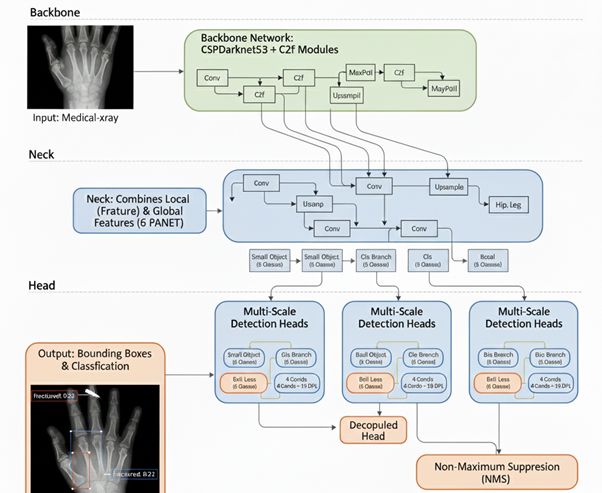
\includegraphics[width=\linewidth]{assets/yolo-arch.png}
	\caption{General architecture of YOLOv8 illustrating the backbone, neck, and detection head components.}
	\label{fig:yolo-arch}
\end{figure}

Object detection has become one of the most important computer vision tasks in modern medical image analysis due to its ability to simultaneously identify and localize pathological findings within an image. Unlike conventional image classification models that only determine whether a disease is present, object detection models additionally provide spatial information regarding the location of abnormalities. This capability is particularly valuable in lung cancer diagnosis, where clinicians must not only determine the presence of a suspicious lesion but also identify its precise location within the lungs.

In the proposed framework, lung cancer detection is formulated as an object detection problem rather than a traditional image classification task. Instead of predicting a single label for an entire CT scan, the model identifies suspicious cancerous regions and generates bounding boxes surrounding them. To accomplish this task, the proposed system employs YOLOv8 (You Only Look Once Version 8), one of the most recent and advanced members of the YOLO family of object detection architectures.

YOLOv8 is a single-stage object detector, meaning that object localization and classification are performed within a single forward pass through the network. This design significantly reduces computational complexity compared to two-stage detectors such as Faster R-CNN, which first generate candidate regions and subsequently classify them. By combining both operations into a unified architecture, YOLOv8 achieves high detection accuracy while maintaining efficient inference speeds. These characteristics make it particularly suitable for deployment within real-time clinical decision support systems where rapid analysis of CT scans is desirable.

The complete processing pipeline employed by the proposed lung cancer detection model is illustrated in Figure~\ref{fig:yolo_pipeline}.

\begin{figure}[H]
	\centering
	
	\resizebox{\linewidth}{!}{
		\begin{tabular}{c c c c c c c c c c c}
			\fbox{
				\begin{tabular}{c}
					Chest CT\\
					Input
				\end{tabular}
			}
			&
			$\rightarrow$
			&
			\fbox{
				\begin{tabular}{c}
					Image\\
					Preprocessing
				\end{tabular}
			}
			&
			$\rightarrow$
			&
			\fbox{
				\begin{tabular}{c}
					YOLOv8\\
					Backbone
				\end{tabular}
			}
			&
			$\rightarrow$
			&
			\fbox{
				\begin{tabular}{c}
					PANet\\
					Neck
				\end{tabular}
			}
			&
			$\rightarrow$
			&
			\fbox{
				\begin{tabular}{c}
					Detection\\
					Head
				\end{tabular}
			}
			&
			$\rightarrow$
			&
			\fbox{
				\begin{tabular}{c}
					Lung Cancer\\
					Detection
				\end{tabular}
			}
		\end{tabular}
	}
	
	\caption{End-to-end processing pipeline of the proposed YOLOv8 lung cancer detection model.}
	\label{fig:yolo_pipeline}
\end{figure}

As illustrated in Figure~\ref{fig:yolo-arch}, YOLOv8 consists of three primary components: the backbone, the neck, and the detection head. Each component contributes a specific functionality to the overall detection process.

\subsubsection{Backbone Network}

The backbone serves as the feature extraction component of YOLOv8. Its primary objective is to transform raw CT scan images into hierarchical feature representations that can be used for lesion detection. YOLOv8 employs the C2f (Cross-Stage Partial Bottleneck with Two Convolutions) architecture, which is an evolution of the CSP (Cross Stage Partial) designs used in previous YOLO versions.

The backbone progressively applies convolutional operations to the input image, generating increasingly abstract feature maps. Early layers learn low-level visual characteristics such as edges, gradients, and texture variations, while deeper layers capture more complex semantic information associated with pulmonary nodules, masses, and abnormal tissue structures.

One of the key advantages of the C2f architecture is its ability to improve gradient propagation while reducing computational overhead. By reusing features across multiple layers, the network can learn richer representations without requiring excessive numbers of parameters. This characteristic is particularly beneficial in medical imaging applications where datasets are often smaller than those available in general computer vision tasks.

For lung cancer detection, the backbone learns to distinguish subtle visual differences between healthy lung tissue and suspicious lesions. These differences may include variations in density, texture, shape, and intensity patterns that are characteristic of malignant abnormalities.

\subsubsection{Neck Network}

The neck component is responsible for feature aggregation and multi-scale feature fusion. In YOLOv8, this functionality is implemented using a Path Aggregation Network (PANet).

Feature extraction layers at different depths of the backbone capture information at different scales. Shallow layers retain detailed spatial information, while deeper layers capture more abstract semantic features. Because lung cancer lesions can vary significantly in size, relying on a single feature scale would limit detection performance.

Small pulmonary nodules may occupy only a tiny portion of the CT image, whereas larger tumors may extend across substantial regions of the lung. The PANet structure addresses this challenge by combining feature maps generated at multiple scales. Through repeated top-down and bottom-up information flow, PANet enables the model to simultaneously utilize local texture details and broader anatomical context.

Consequently, the neck allows YOLOv8 to detect both small and large lesions while maintaining accurate localization performance across a wide range of tumor sizes.

\subsubsection{Detection Head}

The final component of YOLOv8 is the detection head. This module is responsible for generating the actual predictions produced by the network.

Unlike earlier object detectors that relied on predefined anchor boxes, YOLOv8 employs an anchor-free detection strategy. Rather than predicting offsets relative to predetermined anchors, the model directly predicts object centers and bounding box coordinates.

The detection head performs two independent tasks:

\begin{itemize}
	\item Classification of detected regions.
	\item Localization of detected lesions.
\end{itemize}

This decoupled architecture allows each task to be optimized independently, improving overall detection performance. For each detected region, the model predicts:

\begin{itemize}
	\item Bounding box coordinates.
	\item Object confidence score.
	\item Cancer detection probability.
\end{itemize}

The resulting predictions are then forwarded to the post-processing stage for refinement.

\subsubsection{Multi-Scale Detection}

A major challenge in lung cancer detection is the substantial variability in lesion size. Early-stage tumors may appear as extremely small nodules, whereas advanced-stage tumors can occupy large portions of the lung field.

YOLOv8 addresses this challenge through multi-scale detection. Detection heads operate on feature maps of different resolutions, enabling the model to identify abnormalities across multiple spatial scales.

This capability is particularly important in CT-based diagnosis because the early detection of small nodules is often critical for improving patient outcomes. Multi-scale processing allows the model to preserve fine-grained details while simultaneously leveraging high-level semantic information extracted from deeper network layers.

The full process of multi-scale feature extraction is shown in Figure~\ref{fig:yolo_multiscale}

\begin{figure}[H]
	\centering
	
	\begin{tabular}{ccc}
		
		\fbox{
			\begin{minipage}{0.25\textwidth}
				\centering
				High-Resolution Features\\
				(Small Nodules)
			\end{minipage}
		}
		
		&
		
		\fbox{
			\begin{minipage}{0.25\textwidth}
				\centering
				Medium-Resolution Features\\
				(Intermediate Lesions)
			\end{minipage}
		}
		
		&
		
		\fbox{
			\begin{minipage}{0.25\textwidth}
				\centering
				Low-Resolution Features\\
				(Large Tumors)
			\end{minipage}
		}
		
	\end{tabular}
	
	\vspace{0.5cm}
	
	$\downarrow$
	
	\vspace{0.3cm}
	
	\fbox{
		\begin{minipage}{0.4\textwidth}
			\centering
			Unified Multi-Scale Detection Output
		\end{minipage}
	}
	
	\caption{Multi-scale feature extraction employed by YOLOv8 for detecting lung lesions of varying sizes.}
	\label{fig:yolo_multiscale}
\end{figure}

\subsubsection{Anchor-Free Detection Mechanism}

Traditional object detection models rely on predefined anchor boxes that attempt to approximate the expected shapes and sizes of target objects. Although effective in many applications, anchor-based methods introduce additional hyperparameters and often struggle with irregularly shaped objects.

Lung tumors exhibit substantial variability in morphology and rarely conform to standardized geometric patterns. Consequently, anchor-based approaches may fail to adequately represent their boundaries.

YOLOv8 addresses this limitation by adopting an anchor-free detection strategy. Instead of matching objects to predefined anchor templates, the model directly predicts object centers and corresponding bounding box coordinates.

This design offers several advantages:

\begin{itemize}
	\item Reduced hyperparameter complexity.
	\item Improved adaptability to irregular tumor shapes.
	\item Faster convergence during training.
	\item Enhanced localization performance.
\end{itemize}

These characteristics make anchor-free detection particularly suitable for medical imaging applications involving heterogeneous pathological structures.

\subsubsection{Bounding Box Regression and Localization}

Once suspicious regions have been identified, YOLOv8 must determine the exact boundaries of each lesion.

Bounding box regression is performed by predicting:

\begin{itemize}
	\item Horizontal position.
	\item Vertical position.
	\item Width.
	\item Height.
\end{itemize}

These predictions are continuously refined throughout training using specialized localization loss functions. The resulting bounding boxes provide interpretable visual evidence regarding the location of suspicious findings and can assist clinicians during diagnostic review.

\subsubsection{Non-Maximum Suppression}

Object detectors frequently generate multiple overlapping predictions for the same lesion. To eliminate redundant detections, YOLOv8 employs Non-Maximum Suppression (NMS).

The process is illustrated in Figure~\ref{fig:yolo_nms}.

\begin{figure}[H]
	\centering
	
	\resizebox{0.95\linewidth}{!}{
		\begin{tabular}{c c c c c c c}
			
			\fbox{
				\begin{tabular}{c}
					Overlapping\\
					Bounding Boxes
				\end{tabular}
			}
			
			&
			$\rightarrow$
			&
			
			\fbox{
				\begin{tabular}{c}
					IoU\\
					Calculation
				\end{tabular}
			}
			
			&
			$\rightarrow$
			&
			
			\fbox{
				\begin{tabular}{c}
					Non-Maximum\\
					Suppression
				\end{tabular}
			}
			
			&
			$\rightarrow$
			&
			
			\fbox{
				\begin{tabular}{c}
					Final Lung Cancer\\
					Detection
				\end{tabular}
			}
			
		\end{tabular}
	}
	
	\caption{Non-Maximum Suppression procedure used to remove duplicate detections and retain the highest-confidence prediction.}
	\label{fig:yolo_nms}
\end{figure}

The overlap between predicted and ground-truth boxes is measured using the Intersection over Union (IoU) metric:

\[
IoU =
\frac
{
	Area(B_p \cap B_g)
}
{
	Area(B_p \cup B_g)
}
\]

where \(B_p\) denotes the predicted bounding box and \(B_g\) denotes the ground-truth bounding box.

Predictions with excessive overlap are suppressed, ensuring that each lesion is represented by a single final detection.

\subsubsection{Training Objective and Loss Functions}

YOLOv8 optimizes a composite loss function composed of multiple components.

\paragraph{Classification Loss (Binary Cross-Entropy)}

Binary Cross-Entropy loss guides the model in distinguishing cancerous lesions from background regions. This loss encourages accurate classification while minimizing false positive detections.

\paragraph{Box Localization Loss (CIoU)}

Complete Intersection over Union (CIoU) loss evaluates localization quality by considering overlap area, center distance, and aspect ratio differences between predicted and ground-truth boxes.

This loss can be expressed conceptually as:

\[
L_{CIoU}
=
1 - IoU
+
\text{Distance Penalty}
+
\text{Aspect Ratio Penalty}
\]

where additional penalty terms improve localization precision.

\paragraph{Distribution Focal Loss (DFL)}

Distribution Focal Loss improves boundary estimation by modeling uncertainty in bounding box coordinates. This is particularly important in medical images where lesion boundaries may be ambiguous or partially obscured.

Together, these loss functions allow YOLOv8 to simultaneously optimize classification accuracy and localization quality.

\subsubsection{Suitability of YOLOv8 for Lung Cancer Detection}

Several characteristics make YOLOv8 particularly suitable for lung cancer detection.

First, its single-stage architecture provides rapid inference speeds while maintaining high detection accuracy. This allows the model to be integrated into real-time diagnostic support systems.

Second, multi-scale feature extraction enables the detection of lesions exhibiting substantial size variation, ranging from small pulmonary nodules to larger malignant masses.

Third, the anchor-free detection mechanism improves adaptability to irregular tumor morphologies commonly encountered in clinical practice.

Fourth, the generated bounding boxes provide intuitive visual explanations that can assist clinicians in understanding and verifying model predictions.

Finally, YOLOv8 benefits from transfer learning, allowing knowledge acquired from large-scale image datasets to be leveraged for medical imaging tasks. This capability is especially valuable when working with limited annotated medical datasets.

To evaluate the effectiveness of the proposed lung cancer detection model, Precision, Recall, and mAP50 are employed as the primary performance metrics. Precision quantifies the proportion of detected lesions that are truly cancerous, Recall measures the proportion of actual lesions successfully identified by the model, and mAP50 provides a comprehensive assessment of overall detection performance by evaluating both localization and classification accuracy at an Intersection over Union threshold of 0.50.

Collectively, these metrics provide a rigorous evaluation of the model's ability to accurately identify and localize lung cancer lesions within chest CT scans, ensuring that the resulting system can serve as a reliable component of the proposed intelligent diagnostic framework.

\subsection{The CheXFound Vision Foundation Model and ViT Architecture}
\label{subsec:chexfound_vit}

To address the limitations of centralized and domain-restricted architectures under severe data siloing, modern clinical pipelines are shifting toward Vision Foundation Models (VFMs). At the forefront of this shift is \textbf{CheXFound}, a self-supervised, vision-centric foundation model engineered explicitly for high-throughput, multi-class thoracic imaging diagnosis. CheXFound eliminates the historical constraint of training standalone networks for separate diagnostic indications by building generalized, highly robust chest representations. By utilizing a heavy Vision Transformer (ViT) architecture rather than a conventional convolutional backbone, CheXFound effectively captures long-range dependencies, contextual anatomical relationships, and fine-grained pathological variations across heterogeneous image streams.

\subsubsection{The Vision Transformer (ViT-Large) Backbone Architecture}

CheXFound is structurally built upon a modified \textbf{ViT-Large (ViT-L/16)} structural spine, optimizing representation capabilities at an expanded spatial resolution of $512\times512$ pixels. This configuration is mathematically designed to process image grids without losing subtle pathological signals, such as micro-nodular patterns or faint ground-glass borders, which often disappear when compressed into lower-resolution latent matrices. 

The structural flow of the forward pass within CheXFound's ViT-L/16 architecture proceeds as follows:

\begin{enumerate}
	\item \textbf{Patch Extraction and Flattening:} A continuous two-dimensional input thoracic image $\mathbf{X} \in \mathbb{R}^{H \times W \times C}$ (where $H=W=512$ and $C=1$ for radiographs or single-slice CTs) is systematically split into a grid of non-overlapping, uniform rectangular patches $\mathbf{X}_p \in \mathbb{R}^{N \times (P^2 \cdot C)}$. Here, $P = 16$ denotes the hardcoded spatial patch size, and $N$ represents the resulting total number of sequence patches, computed mathematically as:
	\begin{equation}
		N = \frac{H \cdot W}{P^2} = \frac{512 \times 512}{16 \times 16} = 1024 \text{ patches}
	\end{equation}
	
	\item \textbf{Linear Patch Embedding:} Each flattened structural patch token is projected into a lower-dimensional latent embedding space using a trainable linear mapping matrix $\mathbf{E} \in \mathbb{R}^{(P^2 \cdot C) \times D}$, where $D = 1024$ defines the dense hidden embedding dimension of the ViT-Large backbone.
	
	\item \textbf{CLS Token Prepended and Position Encodings:} A learnable classification token embedding $\mathbf{z}_0^0 = \mathbf{x}_{\text{class}} \in \mathbb{R}^D$ is prepended to the sequence of patch tokens. To preserve the two-dimensional spatial topography of the chest inside a one-dimensional sequence pipeline, standard learnable one-dimensional position encodings $\mathbf{E}_{\text{pos}} \in \mathbb{R}^{(N+1) \times D}$ are element-wise added to the patch embeddings, yielding the initial input tensor $\mathbf{z}_0$:
	\begin{equation}
		\mathbf{z}_0 = \left[ \mathbf{x}_{\text{class}}; \, \mathbf{X}_p^1\mathbf{E}; \, \mathbf{X}_p^2\mathbf{E}; \, \dots; \, \mathbf{X}_p^N\mathbf{E} \right] + \mathbf{E}_{\text{pos}}
	\end{equation}
	
	\item \textbf{Transformer Encoder Blocks:} The combined sequence $\mathbf{z}_0$ passes sequentially through $L = 24$ identical Transformer Encoder blocks. Each block features a Multi-Head Self-Attention (\text{MHSA}) mechanism with $h = 16$ distinct attention heads, interleaved with Multi-Layer Perceptron (\text{MLP}) blocks and scaled by Layer Normalization (\text{LN}) using residual skip-connections:
	\begin{align}
		\mathbf{z}_{\ell}' &= \text{MHSA}(\text{LN}(\mathbf{z}_{\ell-1})) + \mathbf{z}_{\ell-1}, \quad \ell = 1, \dots, 24 \\
		\mathbf{z}_{\ell} &= \text{MLP}(\text{LN}(\mathbf{z}_{\ell}')) + \mathbf{z}_{\ell}'
	\end{align}
\end{enumerate}

The standard ViT core configuration embedded inside CheXFound is mathematically mapped and detailed in Table~\ref{tab:vit_large_specs}.

\begin{table}[htbp]
	\centering
	\caption{Structural and mathematical parameter configurations of the CheXFound ViT-Large/16 backbone layout.}
	\label{tab:vit_large_specs}
	\small
	\begin{tabularx}{\textwidth}{lXX}
		\toprule
		\textbf{Architectural Hyperparameter} & \textbf{Formal Definition / Notation} & \textbf{Deterministic Global Value} \\
		\midrule
		\textbf{Input Resolution} & $H \times W \times C$ & $512 \times 512 \times 1$ Pixels \\
		\addlinespace
		\textbf{Patch Dimension} & $P \times P$ & $16 \times 16$ Pixels \\
		\addlinespace
		\textbf{Sequence Count} & $N = (H \cdot W)/P^2$ & $1024$ Active Patch Tokens \\
		\addlinespace
		\textbf{Hidden Layer Dimension} & $D$ & $1024$ Scaled Scaling Dimensions \\
		\addlinespace
		\textbf{Transformer Layers} & $L$ & $24$ Cascaded Encoder Blocks \\
		\addlinespace
		\textbf{Attention Heads} & $h$ & $16$ Independent Heads \\
		\addlinespace
		\textbf{MLP Expansion Ratio} & $\text{Ratio}_{\text{MLP}}$ & $4.0 \times D$ ($4096$ Hidden Units) \\
		\bottomrule
	\end{tabularx}
\end{table}

\subsubsection{Pretraining Paradigm and Self-Supervised Objective Functions}

CheXFound is pretrained on a curated, large-scale medical dataset comprising approximately 987,000 unique chest radiographs derived from 12 distinct open-source clinical databases (including MIMIC-CXR, CheXpert, PadChest, and BraX). To extract optimal task-agnostic representations without relying on manual labels, CheXFound utilizes the **DINOv2** self-supervised learning pipeline. This setup combines a student network (parameterized by weights $\theta_s$) and a teacher network (parameterized by weights $\theta_t$). The teacher's weights are updated continuously via an Exponential Moving Average (EMA) of the student's weights:
\begin{equation}
	\theta_t \leftarrow \lambda \theta_t + (1 - \lambda)\theta_s
\end{equation}

The optimization function combines a multi-crop global-to-local cross-entropy loss with an explicit Masked Image Modeling (MIM) autoencoder objective function. Given a global view image input $x_g$ and a local masked crop input $x_l$, the multi-crop cross-entropy loss enforces representational consistency across scales:
\begin{equation}
	\mathcal{L}_{\text{global}} = \sum_{x \in \{x_g, x_l\}} \sum_{i \neq j} H\left(P_t(x^{(i)}), P_s(x^{(j)})\right)
\end{equation}
where $H(p, q) = -p \log q$, and $P_t, P_s$ denote the soft probability outputs generated by passing the $\mathbf{x}_{\text{class}}$ token through a centering and sharpening bottleneck.

Concurrently, the MIM objective function randomly masks out a subset of the patch sequence tokens (typically 50\% bounding ratios) before feeding them into the student network. The model then computes a localized categorical cross-entropy loss at the patch-token level against the unmasked teacher representations, training the model to predict contextual structure:
\begin{equation}
	\mathcal{L}_{\text{MIM}} = -\sum_{k \in \mathcal{M}} P_t(\mathbf{z}_k) \log P_s(\mathbf{z}_k)
\end{equation}
where $\mathcal{M}$ signifies the set of index fields tracking the masked patches. The unified self-supervised optimization equation for the foundation layer is structured as:
\begin{equation}
	\mathcal{L}_{\text{CheXFound}} = \alpha \mathcal{L}_{\text{global}} + \beta \mathcal{L}_{\text{MIM}}
\end{equation}

\subsubsection{Global and Local Representations Integration (GLoRI) Downstream Adaptation Head}

Standard foundation models often lose small-scale, localized pathological indicators—such as early-stage lung cancer nodules or subtle tuberculous cavities—during global attention pooling over the classification token ($\mathbf{x}_{\text{class}}$). To prevent this loss, CheXFound introduces a specialized downstream adaptation module called the **Global and Local Representations Integration (GLoRI)** head. 

Instead of relying solely on the final layer's $\mathbf{x}_{\text{class}}$ token, the GLoRI module processes both coarse-grained global features and fine-grained, localized patch tokens. During downstream fine-tuning, the backbone CheXFound parameters remain completely frozen to preserve generalizability, while the GLoRI head operates as a trainable multi-head cross-attention layer.

The mathematical routing within the GLoRI module follows this pipeline:
\begin{enumerate}
	\item The global representation vector $\mathbf{f}_g \in \mathbb{R}^D$ is isolated from the class token $\mathbf{x}_{\text{class}}$.
	\item The array of patch tokens $\mathbf{F}_p = [\mathbf{z}_1, \mathbf{z}_2, \dots, \mathbf{z}_1024] \in \mathbb{R}^{1024 \times D}$ is mapped to extract high-resolution localized profiles.
	\item A specific cross-attention layer treats the global feature vector as the query vector ($\mathbf{Q}$), while mapping the patch tokens to generate the keys ($\mathbf{K}$) and values ($\mathbf{V}$):
	\begin{equation}
		\mathbf{Q} = \mathbf{f}_g \mathbf{W}_Q, \quad \mathbf{K} = \mathbf{F}_p \mathbf{W}_K, \quad \mathbf{V} = \mathbf{F}_p \mathbf{W}_V
	\end{equation}
	where $\mathbf{W}_Q, \mathbf{W}_K, \mathbf{W}_V$ represent trainable projection matrices with 8 attention heads and a multi-head channel layout of 786 units.
	
	\item The final contextual integrated vector $\mathbf{f}_{\text{GLoRI}}$ is computed via scaled dot-product attention, blending global context with localized pathology indicators:
	\begin{equation}
		\mathbf{f}_{\text{GLoRI}} = \text{Softmax}\left(\frac{\mathbf{Q}\mathbf{K}^T}{\sqrt{d_k}}\right)\mathbf{V} + \mathbf{f}_g
	\end{equation}
\end{enumerate}

Figure~\ref{fig:chexfound_glori_flow} illustrates the workflow of the input transformation, patching layer, ViT matrix encoding, and the GLoRI feature blending architecture within the system.

\begin{figure}[H]
	\centering
	% Scaled to 0.73 and tightly condensed node gaps to prevent horizontal page overflow
	\begin{tikzpicture}[scale=0.73, transform shape, node distance=1.0cm and 0.8cm, auto, >=latex, font=\small]
		% Modern TikZ styles definition
		\tikzset{
			block/.style={rectangle, draw, fill=blue!10, text width=7em, text centered, rounded corners, minimum height=3.5em},
			cloud/.style={rectangle, draw, fill=green!10, text width=8em, text centered, rounded corners, minimum height=3.5em},
			process/.style={rectangle, draw, fill=orange!10, text width=8em, text centered, minimum height=3.5em}
		}
		
		% Row 1: Global Token Path (Top)
		\node [process] (cls) {Global Token\\($x_{\text{class}} \in \mathbb{R}^{1024}$)};
		
		% Row 2: Core Backbone Flow (Middle)
		\node [block, below=of cls, yshift=0.15cm] (vit) {ViT-Large\\Encoder ($L=24$)};
		\node [block, left=of vit] (patch) {Patch Splitter\\($16 \times 16$ Patches)};
		\node [block, left=of patch] (input) {Input Image\\($512 \times 512$)};
		
		\node [cloud, right=of vit, xshift=0.5cm] (glori) {GLoRI Cross-Attention Head};
		\node [cloud, right=of glori] (output) {Multi-Class\\Disease Output};
		
		% Row 3: Local Patches Path (Bottom)
		\node [process, below=of vit, yshift=-0.15cm] (patches) {Local Patches\\($F_p \in \mathbb{R}^{1024 \times 1024}$)};
		
		% Edges & Connections
		\draw [->, thick] (input) -- (patch);
		\draw [->, thick] (patch) -- (vit);
		
		% Routing from Encoder to the split rows
		\draw [->, thick] (vit) -- (cls);
		\draw [->, thick] (vit) -- (patches);
		
		% Routing from split rows into GLoRI module
		\draw [->, thick] (cls) -| node[pos=0.4, above] {Query ($Q$)} (glori);
		\draw [->, thick] (patches) -| node[pos=0.4, below] {Keys/Values ($K,V$)} (glori);
		
		\draw [->, thick] (glori) -- (output);
	\end{tikzpicture}
	\caption{Functional computational pipeline of the CheXFound framework: Transitioning from input image patch serialization, through the ViT-Large encoder blocks, to the GLoRI cross-attention alignment module.}
	\label{fig:chexfound_glori_flow}
\end{figure}

Furthermore, Figure~\ref{fig:chexfound_placeholder} serves as a modular architectural block diagram tracking the data flow from structural raw DICOM files to final predictions.

\begin{figure}[H]
	\centering
	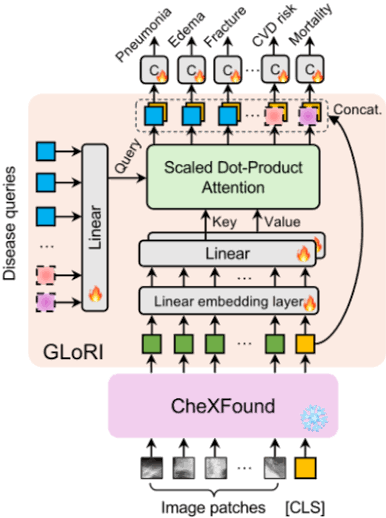
\includegraphics[width=\linewidth]{assets/vit-1.png}
	\caption{Modular schematic layout detailing parameter extraction, input token construction, and feature routing pathways between the frozen base model and the target task head.}
	\label{fig:chexfound_placeholder}
\end{figure}

\section{Medical Image Routing Model}
This section presents the proposed medical image routing model employed in the system and discusses the motivation behind the model, its problem formulation, and finally its architecture. This model serves as the decision-making unit of the system, where the destination of each input image is determined and forwarded thereafter.

\subsection{Motivation}
The increasing use of deep learning in medical image analysis has enabled the development of highly specialized models for tasks such as disease detection and diagnosis. In the context of lung cancer detection, chest X-ray and computed tomography (CT) images provide complementary diagnostic information and often require different processing pipelines and model architectures. While chest X-rays offer a low-cost and widely accessible imaging modality for preliminary screening, CT scans provide detailed cross-sectional information that supports more comprehensive assessment of lung abnormalities.

However, in real-world deployment scenarios, diagnostic systems are often exposed to heterogeneous image inputs originating from different imaging modalities, anatomical regions, or acquisition protocols. Applying a modality-specific diagnostic model to an inappropriate image type may lead to unreliable predictions and compromise the robustness and safety of the overall system. Consequently, there is a need for an initial classification mechanism capable of identifying the nature of incoming medical images before further analysis is performed.

This section introduces a medical image classification model designed to function as an image routing component within a larger lung cancer diagnostic pipeline. The model distinguishes between chest X-ray images, chest CT scan images, and an additional out-of-distribution category referred to as “Other.” By incorporating this third category, the system is able to explicitly handle images that do not belong to the intended diagnostic classes, thereby reducing the risk of misclassification and improving overall system reliability. Once classified, chest X-ray and CT scan images are forwarded to their corresponding lung cancer diagnostic models, while out-of-distribution images are rejected from further analysis. The following subsections present the motivation for this approach, formally define the classification problem, and describe the model architecture employed.

\subsection{Problem Statement}

The goal of this work is to develop an automated medical image classification model capable of identifying the type of an input image and routing it to the appropriate downstream analysis. The task is formulated as a three-class classification problem, where each input image \(X \in \mathbb{R}^{224 \times 224 \times 3}\) must be assigned to one of three categories: chest X-ray images (\(0\)), chest CT scan images (\(1\)), or out-of-distribution images labeled as \emph{Other} (\(2\)). This multi-class formulation ensures that irrelevant or ambiguous inputs are explicitly handled, improving system safety and reducing the risk of inappropriate downstream processing.

The model is designed to output a probability distribution \(\mathbf{p} = [p_0, p_1, p_2]\) over the three classes, where \(p_k = P(y = k \mid X)\) and \(\sum_{k=0}^{2} p_k = 1\). The predicted class is obtained by selecting the class with the highest probability, \(\hat{y} = \arg\max_{k} p_k\). Images classified as chest X-rays are forwarded to the X-ray-based lung cancer detection model, while images classified as CT scans are routed to the CT-based lung cancer detection model. By incorporating the \emph{Other} category, the model avoids forcing all inputs into diagnostic categories and can robustly separate images outside the target distribution, laying a solid foundation for safe integration within a larger medical image analysis pipeline.

\subsection{Model Architecture}

The proposed medical image classification model is designed using a transfer learning approach based on the ResNet50 convolutional neural network. The architecture follows a structured pipeline consisting of input preprocessing, deep feature extraction, feature aggregation, and final classification. This modular design allows the model to benefit from representations learned on large-scale image datasets while adapting effectively to the target medical imaging task. An overview of the complete classification pipeline is illustrated in Figure~\ref{fig:overall_architecture}.

\begin{figure}[h]
	\centering
	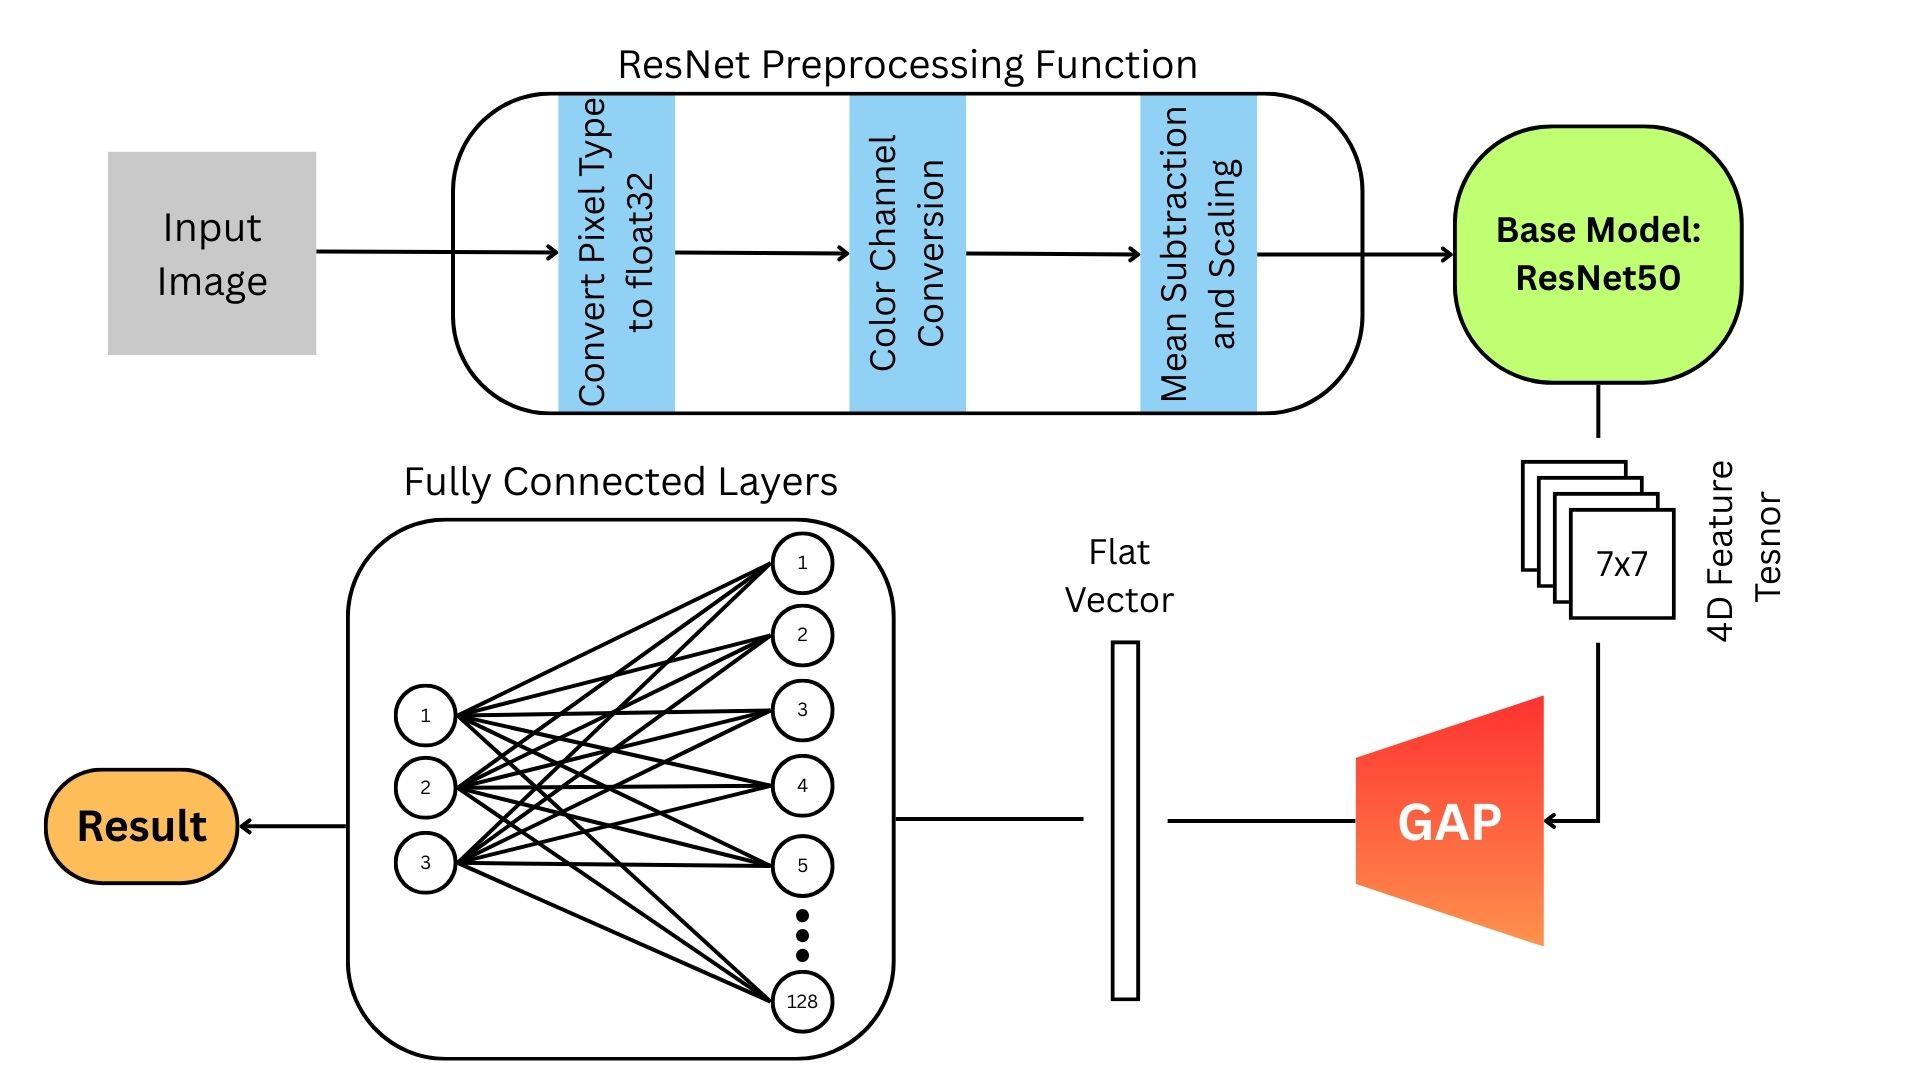
\includegraphics[width=0.95\linewidth]{assets/router-architecture.jpg}
	\caption{Overall architecture of the proposed medical image routing model.}
	\label{fig:overall_architecture}
\end{figure}

The input to the model is a medical image \(X \in \mathbb{R}^{224 \times 224 \times 3}\), resized to a fixed spatial resolution and represented in RGB color space. Prior to being processed by the pretrained network, the image undergoes a preprocessing step to ensure compatibility with the ResNet50 weights. This step mirrors the preprocessing applied during the original ImageNet training of ResNet50 and is essential for effective transfer learning. Specifically, the input image is first converted to floating-point representation, its color channels are reordered from RGB to BGR, and a fixed channel-wise mean is subtracted. Let \(X_{rgb}\) denote the raw input image; the preprocessed image \(X_{prep}\) is obtained as \(X_{prep} = \mathrm{BGR}(X_{rgb}) - \mu\), where \(\mu = [103.939, 116.779, 123.68]\) represents the ImageNet mean for the blue, green, and red channels, respectively. This operation centers the input distribution around zero and aligns it with the statistical properties expected by the pretrained backbone.

Following preprocessing, the image is passed through the ResNet50 network with its original classification layers removed. In this configuration, ResNet50 functions as a fully convolutional feature extractor. For an input tensor of shape \((224, 224, 3)\), the output of the backbone is a high-dimensional feature map of shape \((7, 7, 2048)\). This tensor contains 2048 feature channels, each encoding abstract visual patterns such as anatomical structures, textures, and modality-specific characteristics while preserving coarse spatial relationships within the image. For a detailed discussion of the ResNet50 model architecture, refer to Subsection~\ref{subsec:resnet50-arch}.

To transform the spatial feature maps into a compact representation suitable for classification, a global average pooling operation is applied to the output of the ResNet50 backbone. This operation computes the average activation of each feature channel across the spatial dimensions, effectively summarizing the presence of each learned feature over the entire image. Given a feature map \(F \in \mathbb{R}^{7 \times 7 \times 2048}\), the pooled feature vector \(z \in \mathbb{R}^{2048}\) is computed such that each element \(z_k\) corresponds to the mean of the activations in channel \(k\), i.e.
\begin{equation*}
	z_k = \frac{1}{7 \times 7} \sum_{i=1}^{7} \sum_{j=1}^{7} F_{i,j,k}
\end{equation*}
This operation reduces the tensor shape from \((7, 7, 2048)\) to \((2048)\) while significantly lowering the number of parameters required in subsequent layers and improving generalization.

The resulting feature vector is then passed to a task-specific classification head composed of fully connected layers. These layers learn discriminative combinations of the extracted features and map them to the target class space. The final layer applies a softmax activation function, producing a probability distribution \(\mathbf{p} = [p_0, p_1, p_2]\), where each component represents the predicted probability of the image belonging to the chest X-ray class, chest CT scan class, or the out-of-distribution \emph{Other} class. The predicted label is obtained as \(\hat{y} = \arg\max_k p_k\).


\section{Chest Disease Classification Model}

This section presents one of the downstream diagnostic models developed within the project, focusing on automated multi-class classification of chest diseases from chest X-ray (CXR) images. The model is designed as a robust and interpretable pipeline that integrates standardized image preprocessing, lung region isolation, and deep learning–based classification using transfer learning. Emphasis is placed on architectural design choices and methodological foundations rather than performance evaluation, which is discussed in a later chapter.

\subsection{Motivation}

Deep learning has demonstrated strong potential in medical image analysis, yet several challenges remain, including variability in image acquisition, class imbalance, and the need for explainable decision-making. The proposed model addresses these issues through a multi-stage pipeline that enhances image quality, isolates clinically relevant lung regions, and applies a transfer learning–based classifier augmented with explainability techniques.

\subsection{Problem Statement}

The objective of this model is to perform multi-class classification of chest X-ray images into the following diagnostic categories:
\[
\mathcal{C} = \{\text{NORMAL}, \text{PNEUMONIA}, \text{COVID-19}, \text{TUBERCULOSIS}\}.
\]

Given an input chest X-ray image \( I \in \mathbb{R}^{H \times W} \), the task is to learn a mapping
\[
f_\theta : I \rightarrow \mathbf{p},
\]
where \( \mathbf{p} \in \mathbb{R}^{|\mathcal{C}|} \) is a probability distribution over disease classes and \( \theta \) denotes the model parameters.

To improve robustness and clinical relevance, the classification task is constrained to lung parenchyma regions extracted via an explicit segmentation stage. Additionally, the model must provide interpretable outputs to support clinical trust, motivating the use of gradient-based visualization techniques.

\subsection{Model Architecture}

The diagnostic model is structured as a multi-stage pipeline, illustrated conceptually in Figure~\ref{fig:chest_pipeline_overview}. The pipeline consists of three main components: image preprocessing, lung segmentation, and disease classification.


\begin{figure}[h]
	\centering
	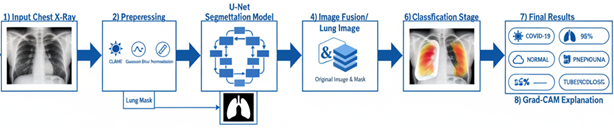
\includegraphics[width=0.75\textwidth]{assets/chest-pipeline.png}
	\caption{High-level overview of the multi-stage chest disease classification pipeline.}
	\label{fig:chest_pipeline_overview}
\end{figure}


Each chest X-ray image undergoes a standardized preprocessing pipeline to enhance diagnostically relevant features. Images are first converted to grayscale and enhanced using Contrast Limited Adaptive Histogram Equalization (CLAHE). Noise introduced during enhancement is mitigated using Gaussian smoothing with a \(5 \times 5\) kernel.

Pixel intensities are then normalized using Min--Max normalization: $I_{\text{norm}} = \frac{I - I_{\min}}{I_{\max} - I_{\min}}$ where \( I_{\min} \) and \( I_{\max} \) represent the minimum and maximum pixel values of the image. Finally, images are converted to RGB format to ensure compatibility with the ResNet50 model. For a discussion of the ResNet50 model, refer to Subsection~\ref{subsec:resnet50-arch}.

Figure~\ref{fig:preprocessing} illustrates the effect of the preprocessing pipeline on representative CXR images.

\begin{figure}[h]
	\centering
	\begin{subfigure}[b]{0.25\textwidth}
		\centering
		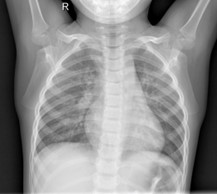
\includegraphics[width=\textwidth]{assets/pneu1.jpg}
		\caption{Original Pneumonia CXR}
		\label{fig:orig-pneumonia}
	\end{subfigure}
	\hspace*{1cm}
	\begin{subfigure}[b]{0.25\textwidth}
		\centering
		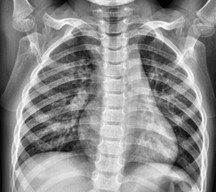
\includegraphics[width=\textwidth]{assets/proc-pneu1.jpg}
		\caption{Preprocessed Pneumonia CXR}
		\label{fig:proc-pneumonia}
	\end{subfigure}
	\\
	\begin{subfigure}[b]{0.25\textwidth}
		\centering
		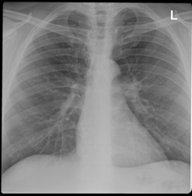
\includegraphics[width=\textwidth]{assets/pneu2.png}
		\caption{Original Pneumonia CXR}
		\label{fig:orig-pneumonia2}
	\end{subfigure}
	\hspace*{1cm}
	\begin{subfigure}[b]{0.25\textwidth}
		\centering
		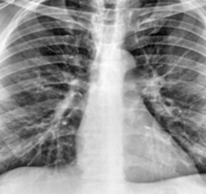
\includegraphics[width=\textwidth]{assets/proc-pneu2.png}
		\caption{Preprocessed Pneumonia CXR}
		\label{fig:proc-pneumonia2}
	\end{subfigure}
	\caption{Chest X-ray images before and after preprocessing, highlighting improved contrast and reduced noise.}
	\label{fig:preprocessing}
\end{figure}
%	\begin{figure}[h]
	%		\centering
	%		\includegraphics[width=0.9\textwidth]{preprocessing_comparison.png}
	%		\caption{Chest X-ray images before and after preprocessing, highlighting improved contrast and reduced noise.}
	%		\label{fig:preprocessing}
	%	\end{figure}

To ensure that classification focuses exclusively on clinically relevant regions, a U-Net–based segmentation model is employed to extract lung masks. The U-Net architecture follows an encoder–decoder structure with skip connections that preserve spatial information, making it well suited for biomedical image segmentation. The U-Net architecture used is shown in Figure~\ref{fig:unet-arch}



\begin{figure}[h]
	\centering
	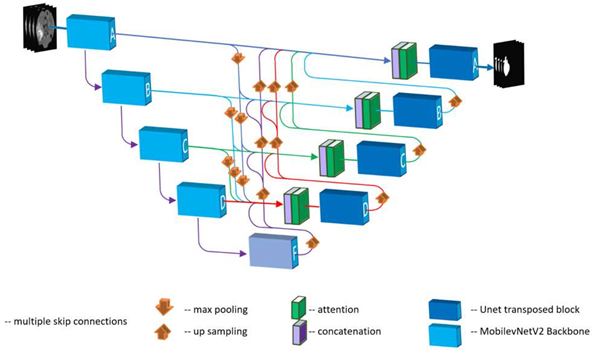
\includegraphics[width=0.9\textwidth]{assets/unet-arch.png}
	\caption{The U-Net architecture, illustrating the encoder-decoder structure with skip connections that merge high-resolution features from the contracting path with upsampled features in the expansive path. This design is highly effective for precise medical image segmentation.}
	\label{fig:unet-arch}
\end{figure}

The segmentation network outputs a binary lung mask \( M \in \{0,1\}^{H \times W} \), which is applied to the preprocessed image using element-wise multiplication:
\[
I_{\text{lung}} = I_{\text{norm}} \odot M.
\]

Training of the segmentation model is guided by the Dice Loss, derived from the Dice--Sørensen Coefficient (DSC):
\[
\text{DSC} = \frac{2|X \cap Y|}{|X| + |Y|},
\]
where \( X \) and \( Y \) denote the predicted and ground-truth masks, respectively. The loss function is defined as
\[
\mathcal{L}_{\text{Dice}} = 1 - \text{DSC},
\]
which is particularly effective in handling class imbalance between lung and background pixels. The result of using segmentation on CXR images is illustrated in Figure~\ref{fig:lung_segmentation}

\begin{figure}[h]
	\centering
	\begin{subfigure}[b]{0.25\textwidth}
		\centering
		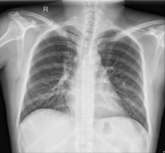
\includegraphics[width=\textwidth]{assets/proc-cxr.png}
		\caption{Preprocessed CXR Image}
		\label{fig:proc-cxr}
	\end{subfigure}
	\hspace*{1cm}
	\begin{subfigure}[b]{0.25\textwidth}
		\centering
		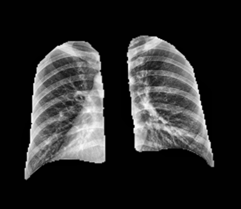
\includegraphics[width=\textwidth]{assets/segmented-lung.png}
		\caption{Segmented Lung Image after Mask Application}
		\label{fig:segmented-lung}
	\end{subfigure}
	\caption{Application of the U-Net segmentation mask. The original preprocessed Figure~\ref{fig:proc-cxr} is processed to produce the final segmented lung Figure~\ref{fig:segmented-lung}, which serves as the input for the classification stage}
	\label{fig:lung_segmentation}
\end{figure}

%	\begin{figure}[h]
	%		\centering
	%		\includegraphics[width=0.9\textwidth]{lung_segmentation.png}
	%		\caption{Application of the U-Net segmentation mask to isolate lung regions from chest X-ray images.}
	%		\label{fig:lung_segmentation}
	%	\end{figure}
%	
The final classification stage employs a ResNet50-based transfer learning model. ResNet architectures leverage residual connections to facilitate gradient flow and enable the training of deep networks. As the ResNet family is discussed in detail earlier in this book, only a brief overview is provided here.

A ResNet50 model pre-trained on ImageNet is used as a feature extractor, with early layers frozen to preserve general visual representations. A custom classification head is appended, consisting of global average pooling, fully connected layers with ReLU activation, dropout for regularization, and a final softmax layer producing class probabilities.

The model is trained using Sparse Categorical Cross-Entropy loss:
\[
\mathcal{L}_{\text{CE}} = - \sum_{i=1}^{N} \log p_{i,c},
\]
where \( p_{i,c} \) denotes the predicted probability of the true class \( c \) for sample \( i \). To address class imbalance, class-weighted loss scaling is applied during training.

To enhance interpretability, Gradient-weighted Class Activation Mapping (Grad-CAM) is employed to visualize the regions most influential to model predictions, an example is shown in Figure~\ref{fig:gradcam}. Grad-CAM computes the gradients of the target class score with respect to the feature maps of the final convolutional layer and produces a coarse localization map highlighting salient regions.

These heatmaps are overlaid on the original chest X-ray images, enabling qualitative assessment of whether the model attends to clinically meaningful lung regions.

\begin{figure}[h]
	\centering
	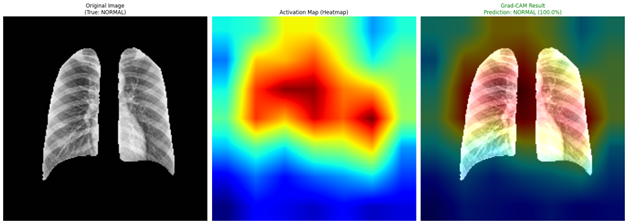
\includegraphics[width=0.9\textwidth]{assets/gradcam.png}
	\caption{Grad-CAM visualizations highlighting regions contributing to model predictions.}
	\label{fig:gradcam}
\end{figure}


\section{Lung Cancer Detection Model}
This section presents the lung cancer and tuberculosis detection model developed within the project, focusing on automated localization and classification of pulmonary abnormalities from chest X-ray (CXR) images[cite: 1, 2]. The model is designed as an end-to-end object detection pipeline that integrates binary mask conversion, bounding box generation, and deep learning–based detection using the YOLOv8 architecture[cite: 3]. Emphasis is placed on the data preparation strategy and architectural design choices that underpin the detection framework[cite: 4].

\subsection{Motivation}
Object detection frameworks offer distinct advantages over image-level classification for medical imaging tasks, as they provide explicit spatial localization of pathological regions rather than a single diagnostic label[cite: 5, 6]. For lung cancer and tuberculosis screening, identifying the precise location and extent of pulmonary lesions or infiltrates is clinically essential, as it directly informs radiological assessment and subsequent clinical decision-making[cite: 7]. The proposed model addresses this requirement by reformulating the diagnostic task as a bounding box regression and classification problem, enabling simultaneous localization and identification of disease regions within a single unified forward pass[cite: 8].

\subsection{Problem Statement}
The objective of this model is to perform multi-class detection of pulmonary abnormalities in chest X-ray images, identifying and localizing instances belonging to the following diagnostic categories[cite: 9, 10]:
\begin{equation}
	C = \{\text{tumor}, \text{tuberculosis}\} [cite: 11]
\end{equation}

Given an input chest X-ray image $I \in \mathbb{R}^{H \times W}$, the task is to learn a mapping[cite: 12]:
\begin{equation}
	f_\theta : I \rightarrow \{(b_i, c_i, s_i)\}_{i=1 \dots N} [cite: 13]
\end{equation}
where each tuple $(b_i, c_i, s_i)$ denotes the predicted bounding box coordinates, class label, and confidence score for the $i$-th detected region, and $\theta$ represents the model parameters[cite: 14].

To bridge the gap between pixel-level segmentation annotations (binary masks) and the bounding box representation required by the detection framework, an explicit mask-to-box conversion stage is incorporated as the first step of the pipeline[cite: 15]. Each connected foreground component in the binary annotation mask is converted into a normalized YOLO-format bounding box, enabling the use of richly annotated mask datasets for detection training without manual re-labeling[cite: 16].

\subsection{Model Architecture}
The detection model is structured as a three-stage pipeline consisting of: (1) mask-to-bounding-box conversion and dataset preparation, (2) YOLO-format data organization and configuration, and (3) YOLOv8-based detection model training and evaluation[cite: 17, 18]. Each stage is described in detail below[cite: 19].

\begin{figure}[htbp]
	\centering
	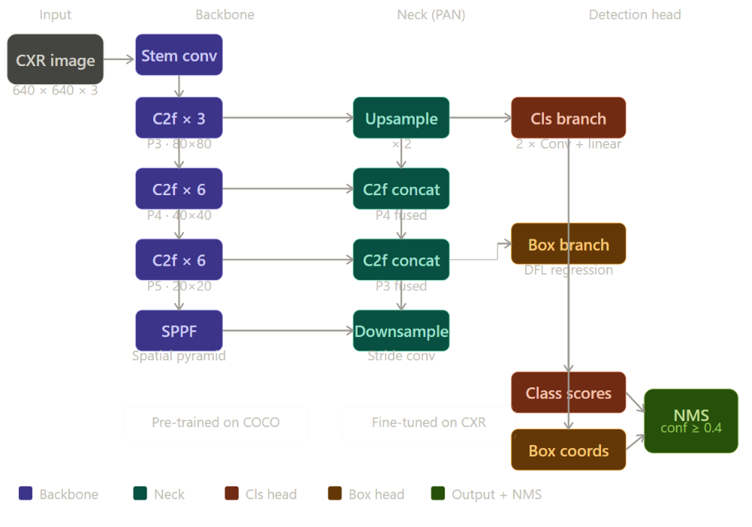
\includegraphics[width=\textwidth]{assets/yolo8_arch.png}
	\caption{YOLOv8 architecture pipeline for automated localization and classification of pulmonary abnormalities.}
	\label{fig:yolov8_architecture}
\end{figure}

\subsubsection{Mask-to-Bounding-Box Conversion}
Annotation masks for pulmonary lesions are provided as binary PNG images in which foreground pixels (intensity $> 127$) correspond to pathological regions[cite: 20, 21]. To convert these masks into YOLO-format bounding box annotations, connected component analysis is applied using external contour detection[cite: 22]. For each detected contour, an axis-aligned bounding box is computed and normalized with respect to the image dimensions, yielding center coordinates and extent values in the range $[0, 1]$[cite: 23].

Formally, for a contour with pixel-space bounding rectangle $(x, y, w, h)$ within an image of width $W$ and height $H$, the normalized YOLO representation is[cite: 24]:
\begin{equation}
	c_x = \frac{x + w/2}{W}, \quad c_y = \frac{y + h/2}{H}, \quad n_w = \frac{w}{W}, \quad n_h = \frac{h}{H} [cite: 25]
\end{equation}

Contours enclosing fewer than 5 pixels in either dimension are discarded as noise prior to annotation generation[cite: 26]. All foreground components within a given mask are assigned the class index corresponding to the image-level label (tumor or tuberculosis), since mask annotations are provided per diagnostic category[cite: 27].

\subsubsection{Dataset Preparation and Splitting}
Following bounding box conversion, the dataset is partitioned into training, validation, and test subsets using stratified random splitting[cite: 28, 29]. The default split proportions are 75\% training, 15\% validation, and 10\% test, with random seed fixed at 42 to ensure reproducibility[cite: 30]. Image files and their corresponding YOLO label files are organized into the standard YOLO directory structure, with separate image and label folders for each split[cite: 31]. A YAML configuration file is generated automatically to specify dataset paths, the number of classes, and class names, serving as the interface between the prepared dataset and the YOLOv8 training framework[cite: 32].

\subsubsection{YOLOv8 Detection Architecture}
Object detection is performed using YOLOv8, the latest generation of the You Only Look Once (YOLO) family of single-stage detectors[cite: 33, 34]. YOLOv8 follows an anchor-free design and adopts a CSPDarknet backbone for feature extraction, a Path Aggregation Network (PAN) neck for multi-scale feature fusion, and a decoupled detection head that separately predicts classification scores and bounding box offsets[cite: 35]. This design enables real-time inference while maintaining competitive localization accuracy[cite: 36].

A YOLOv8n (nano) variant is employed as the base model, pre-trained on the COCO dataset, and fine-tuned on the prepared CXR detection dataset[cite: 37]. The model is trained for 50 epochs with an input resolution of $640 \times 640$ pixels and a batch size of 16[cite: 38]. Transfer learning is leveraged by initializing all network weights from the COCO pre-trained checkpoint, with all layers unfrozen to allow domain-specific adaptation[cite: 38]. The training objective combines binary cross-entropy loss for classification, distribution focal loss (DFL) for bounding box regression, and a complete intersection-over-union (CIoU) penalty term to improve localization precision[cite: 39]:
\begin{equation}
	L = \lambda_{\text{cls}} \cdot L_{\text{cls}} + \lambda_{\text{box}} \cdot L_{\text{box}} + \lambda_{\text{dfl}} \cdot L_{\text{DFL}} [cite: 40]
\end{equation}
where $\lambda_{\text{cls}}$, $\lambda_{\text{box}}$, and $\lambda_{\text{dfl}}$ are scalar weighting coefficients that balance the contribution of each loss component during optimization[cite: 41].

After training, the best-performing checkpoint, selected based on validation mean Average Precision at IoU threshold 0.50 (mAP50), is retained for evaluation[cite: 42]. Model performance is assessed on both the held-out validation and test splits, reporting mAP50, mAP50–95, precision, and recall as primary evaluation metrics[cite: 43]. Qualitative evaluation is conducted by visually inspecting annotated predictions on test set images, examining the spatial correspondence between predicted bounding boxes and known pathological regions[cite: 44].

\begin{figure}[htbp]
	\centering
	\begin{minipage}{0.48\textwidth}
		\centering
		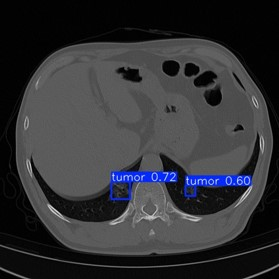
\includegraphics[width=\textwidth]{assets/lung1.jpg}
		\caption{Qualitative evaluation showing tumor localization (confidence scores 0.72 and 0.60) on an axial CT slice.}
		\label{fig:qualitative_ct_1}
	\end{minipage}\hfill
	\begin{minipage}{0.48\textwidth}
		\centering
		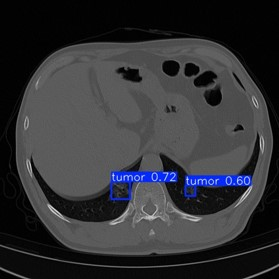
\includegraphics[width=\textwidth]{assets/lung1.jpg}
		\caption{Qualitative evaluation showing tumor localization (confidence score 0.87) on an axial CT slice.}
		\label{fig:qualitative_ct_2}
	\end{minipage}
\end{figure}

\subsection{Interpretability Considerations}
Unlike classification-only models that require post-hoc gradient visualization to identify diagnostically relevant regions, the detection framework provides explicit spatial outputs in the form of bounding boxes and associated confidence scores[cite: 45, 46]. Each prediction directly encodes the model's estimate of where a pathological region is located and how confident it is in that localization[cite: 47]. This built-in spatial explainability reduces the reliance on auxiliary interpretability methods and aligns more naturally with clinical reporting conventions, in which radiologists annotate specific anatomical regions rather than assigning image-level labels[cite: 48]. Confidence thresholding ($\tau = 0.4$) and non-maximum suppression with an IoU threshold of 0.6 are applied at inference time to filter low-quality or redundant detections, producing a concise set of high-confidence predictions per image[cite: 49].

\begin{figure}[htbp]
	\centering
	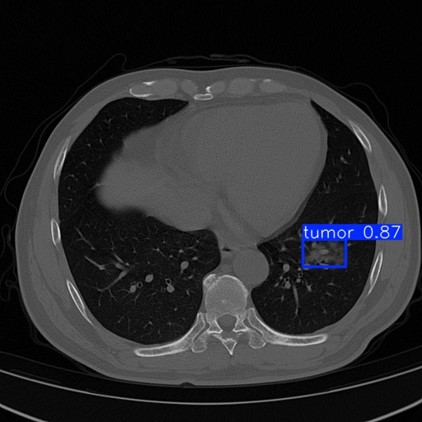
\includegraphics[width=0.6\textwidth]{assets/lung3.jpg}
	\caption{Example of an interpretable YOLO detection result on a chest CT image. The model localizes a suspected lesion using a bounding box and reports a confidence score of 0.87. Such spatial predictions provide inherent interpretability by explicitly identifying the anatomical region associated with the model's decision, reducing the need for post-hoc visualization techniques.}
	\label{fig:interpretability_example}
\end{figure}
\FloatBarrier
\section{Federated Learning}
\subsection{Concept and Motivation}
\label{subsec:fl_concept}
 
Federated learning (FL) is a distributed machine learning paradigm in which
a model is trained collaboratively across multiple independent nodes without
any raw data leaving its source institution~\cite{mcmahan2017}. Rather than
centralizing training samples on a shared server, FL brings the computation
to the data: each participating node trains a local model on its private
dataset and shares only the resulting model parameters with a central
aggregation server, which combines the updates into an improved global model.
This cycle repeats for a defined number of communication rounds until the
global model converges.
 
The motivation for adopting FL in this work is rooted in the fundamental
tension between data-driven model development and patient privacy. Healthcare
institutions collect large volumes of annotated medical images, yet regulatory
frameworks --- including the Health Insurance Portability and Accountability Act
(HIPAA) in the United States and the General Data Protection Regulation (GDPR)
in the European Union --- impose strict constraints on cross-institutional data
sharing. Negotiating data transfer agreements is costly, time-consuming, and
in many cases legally impractical. FL resolves this tension by enabling
institutions to contribute to a shared model without relinquishing data
custody, making large-scale collaborative medical AI both legally feasible
and technically practical.
 
% -----------------------------------------------------------------------------
\subsection{Federated Learning in Medical Imaging}
\label{subsec:fl_medical}
 
The adoption of FL in the medical domain has grown substantially since its
introduction, driven by the recognition that many clinical datasets are too
small at any single institution to train robust deep learning models, while
the combined data across institutions would be sufficient~\cite{sheller2019}.
FL directly addresses this data insufficiency problem without requiring
physical data consolidation.
 
In medical imaging specifically, FL has been applied across a broad range of
modalities and anatomical targets. Early work by Sheller~\textit{et al.}
demonstrated FL for brain tumor segmentation from MRI scans across multiple
institutions, achieving performance comparable to centralized training without
sharing any patient data~\cite{sheller2019}. Subsequent studies have extended
FL to chest radiograph classification, diabetic retinopathy screening from
fundus photography, histopathology slide analysis, and cardiac structure
segmentation from echocardiography, among others~\cite{rieke2020}.
 
This breadth of applicability is a key motivation for the design of the
proposed system. Rather than building a solution tied to a specific model
architecture or anatomical region, the FL framework developed in this work
is designed to be \textbf{model-agnostic} and \textbf{organ-agnostic}: any
classification or segmentation backbone can be substituted as the local
model, and the training data can comprise images from any body region or
imaging modality. The federated coordination layer — covering client
management, weight aggregation, and communication — remains unchanged
regardless of the underlying clinical task.
 
% -----------------------------------------------------------------------------
\subsection{The Federated Averaging Algorithm}
\label{subsec:fedavg}
 
The aggregation algorithm that underpins the proposed system is Federated
Averaging (FedAvg), introduced by McMahan~\textit{et al.}~\cite{mcmahan2017}
and the most widely adopted FL optimization method to date. FedAvg operates
in iterative communication rounds. Let $K$ denote the number of participating
clients, $\mathcal{D}_k$ the private dataset of client $k$, $n_k =
|\mathcal{D}_k|$ its size, and $n = \sum_{k=1}^{K} n_k$ the total number of
training samples across all clients. The global model at round $t$ is
parameterized by weight vector $\mathbf{w}_t$. Each round consists of three
phases:
 
\textbf{(1) Broadcast.} The server distributes the current global model
weights to all $K$ clients:
\begin{equation}
    \mathbf{w}_t \;\longrightarrow\; \{\text{client}_1, \dots, \text{client}_K\}.
\end{equation}
\textbf{(2) Local Training.} Each client $k$ independently minimizes its
local empirical risk $\mathcal{L}_k$ over $E$ local epochs using a gradient-
based optimizer, producing updated local weights:
\begin{equation}
    \mathbf{w}_t^k \;=\; \mathbf{w}_t \;-\; \eta\,\nabla\mathcal{L}_k(\mathbf{w}_t),
\end{equation}
where $\eta$ is the local learning rate and $\mathcal{L}_k$ is the
task-specific loss function evaluated over the client's local dataset:
\begin{equation}
    \mathcal{L}_k(\mathbf{w}) \;=\;
    \frac{1}{n_k}\sum_{(x_i,\,y_i)\,\in\,\mathcal{D}_k}
    \ell\!\left(f_{\mathbf{w}}(x_i),\,y_i\right).
\end{equation}
 
\textbf{(3) Aggregation.} The server collects the locally updated weights
from all clients and computes the new global model as a weighted average
proportional to each client's dataset size:
\begin{equation}
    \mathbf{w}_{t+1} \;=\; \sum_{k=1}^{K}\frac{n_k}{n}\,\mathbf{w}_t^k.
    \label{eq:fedavg}
\end{equation}
This process minimizes the global objective:
\begin{equation}
    F(\mathbf{w}) \;=\; \sum_{k=1}^{K}\frac{n_k}{n}\,\mathcal{L}_k(\mathbf{w}).
\end{equation}
Equation~\eqref{eq:fedavg} assigns greater influence to clients with larger
datasets, which is appropriate in the medical setting where institutional
dataset sizes vary considerably. Clients contributing more annotated images
should exert proportionally greater influence on the global model.
 
% -----------------------------------------------------------------------------
\subsection{Key Parameters of a Federated Learning System}
\label{subsec:fl_parameters}
 
Configuring a federated learning system involves a distinct set of
parameters beyond those of conventional deep learning. These parameters
govern the coordination between server and clients and directly affect
convergence speed, model quality, communication cost, and privacy. A clear
understanding of each parameter is essential for adapting the system to
different clinical tasks. Table~\ref{tab:fl_params} provides an overview
of the critical parameters and their implications.
 
\begin{table}[!htbp]
\centering
\caption{Key Federated Learning Parameters and Their Clinical Implications}
\label{tab:fl_params}
\begin{tabular}{|p{3.2cm}|p{4.2cm}|p{5.8cm}|}
\hline
\textbf{Parameter} & \textbf{Definition} & \textbf{Implication} \\
\hline
Number of clients ($K$)
    & Total participating institutions
    & More clients improve data diversity and model generalization but
      increase coordination overhead. \\
\hline
Communication rounds ($T$)
    & Number of server--client training cycles
    & More rounds improve accuracy at the cost of higher communication
      volume. Convergence is typically monitored to select $T$. \\
\hline
Client fraction ($C$)
    & Proportion of clients selected per round ($C \in (0,1]$)
    & $C = 1.0$ uses all clients every round (synchronous FL).
      $C < 1.0$ enables asynchronous, scalable training. \\
\hline
Local epochs ($E$)
    & Training epochs each client performs before returning weights
    & Higher $E$ reduces communication rounds but risks \textit{client drift}
      — divergence of local models due to non-IID data~\cite{li2020}. \\
\hline
Local batch size ($B$)
    & Mini-batch size for local gradient computation
    & Affects local convergence speed, memory footprint, and gradient
      privacy (smaller batches increase reconstruction attack risk). \\
\hline
Local learning rate ($\eta$)
    & Step size for local gradient updates
    & Must be tuned per model architecture; too large a value exacerbates
      client drift in non-IID settings. \\
\hline
Aggregation strategy
    & Algorithm used to combine client updates (e.g., FedAvg, FedProx,
      FedNova)
    & Choice depends on data heterogeneity; FedAvg is the standard baseline;
      FedProx adds a proximal term to limit client drift. \\
\hline
Data partitioning scheme
    & How training data is divided across clients (IID vs. non-IID)
    & Non-IID partitions (realistic in healthcare) slow convergence and
      reduce final accuracy compared to IID partitions. \\
\hline
Minimum clients for aggregation
    & Minimum number of client updates required before the server aggregates
    & Prevents the global model from being updated on insufficient
      information; critical for stability. \\
\hline
\end{tabular}
\end{table}
 
Among these, the number of local epochs $E$ and the aggregation strategy
warrant particular attention in the medical imaging context. Increasing $E$
reduces the number of costly communication rounds, which is beneficial in
healthcare networks where bandwidth and uptime may be limited. However,
when client datasets are statistically heterogeneous — a common condition
across hospitals using different scanners, populations, or labeling protocols
— high $E$ causes the local models to overfit to their local distributions
and diverge from the global optimum, a phenomenon known as \textit{client
drift}~\cite{li2020}. The selection of $E$ therefore requires careful
empirical tuning for each deployment scenario.
 
% -----------------------------------------------------------------------------
\subsection{System Architecture Overview}
\subsubsection{Client--Server Design}

The system follows a two-tier federated learning architecture implemented using the Flower (\texttt{flwr}) framework. A single Federated Learning (FL) Server process hosts both the Flower gRPC server and a FastAPI-based REST management API within the same Python process. The Flower server operates on port \texttt{50051}, while the REST management layer operates on port \texttt{8001}. Both services share a common \texttt{SharedState} singleton object that stores the current round status, active model type, round identifier, and the reference to the active Flower thread. This co-location eliminates additional network overhead between the aggregation engine and the management layer and enables efficient coordination between both services.

Each participating hospital deploys an FL Client as a Docker container. Upon startup, the client continuously polls the server's health endpoint until a federated learning round becomes active. Once the server signals round activation, the client initializes the appropriate model according to the task being executed. For any task a client model is instantiated. The client subsequently waits for the gRPC service to become available before connecting through Flower's \texttt{NumPyClient} interface.

A key design principle of the architecture is data locality. Medical images and patient records remain exclusively within the hospital infrastructure and are never transmitted to the central server. Instead, only serialized NumPy arrays containing model parameters are exchanged during federated learning rounds. This design significantly reduces privacy risks while maintaining collaborative model training across institutions.

\begin{figure}[H]
	\centering
	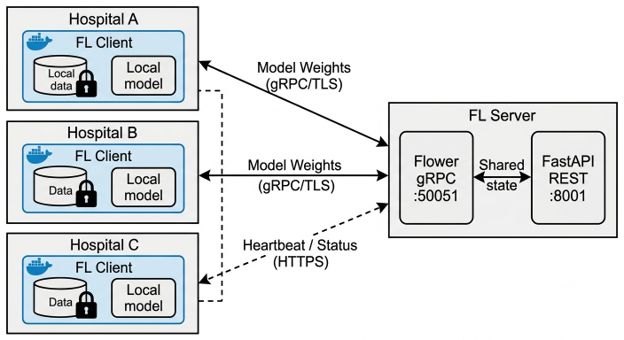
\includegraphics[width=0.9\textwidth]{assets/fl_system_architecture.png}
	\caption{Two-tier federated learning system architecture. Hospital clients communicate with the central federated learning server through TLS-secured gRPC channels, while the REST management layer provides round lifecycle management and monitoring. Raw medical data remains within each hospital boundary.}
	\label{fig:fl_system_architecture}
\end{figure}

\subsubsection{Communication Protocol}

All model parameter exchanges between federated learning clients and the central server are performed using gRPC, Google's high-performance remote procedure call framework built on HTTP/2 and Protocol Buffers. The Flower framework serializes model weight tensors into Protocol Buffer messages before transmission, providing an efficient and platform-independent communication mechanism.

To ensure secure communication, the production deployment uses Transport Layer Security (TLS). Before any model parameters are exchanged, a complete TLS handshake is performed involving a trusted Certificate Authority (CA) certificate, a server certificate, and the server's private key. This process guarantees encrypted communication channels and prevents unauthorized interception or modification of model updates during transmission.

In addition to the gRPC communication channel, the system incorporates a secondary REST-based heartbeat mechanism. Each client periodically sends status reports to the FastAPI management API at a configurable interval, with a default period of 15 seconds. These heartbeat messages include metadata such as the currently active model type and the active federated learning round identifier.

The heartbeat channel provides real-time visibility into client participation and system health while maintaining patient privacy. No medical images, patient records, or other sensitive clinical information are transmitted through this channel. Instead, it serves exclusively for monitoring, synchronization, and lifecycle management purposes.

The server broadcasts the active model type to all clients before the start of each federated learning round. This ensures that all participating institutions instantiate and train identical model architectures, thereby maintaining consistency during the aggregation process.

\subsection{Model Architecture}
\subsubsection{Federated Learning Workflow}

Federated Learning (FL) is a distributed machine learning paradigm that enables multiple clients to collaboratively train a shared global model without directly exchanging their local data. Instead of transferring datasets to a centralized location, each client performs training locally and only shares model updates with a coordinating server. This approach preserves data privacy while allowing the model to benefit from knowledge learned across multiple data sources.

The federated learning process proceeds iteratively through a sequence of communication rounds. At the beginning of each round, the central server distributes the current global model to participating clients. Each client then trains the model on its local dataset and computes updated model parameters. These parameters are subsequently transmitted back to the server, where they are aggregated to produce a new global model.

This collaborative training framework offers several advantages, including improved privacy, reduced data-sharing requirements, and the ability to leverage geographically distributed datasets. As a result, federated learning has become an attractive solution in domains where data governance, confidentiality, or regulatory constraints limit centralized data collection.

\subsubsection{Local Data Processing}

Prior to local training, each client performs preprocessing on its own dataset according to a predefined and consistent pipeline. Standardized preprocessing ensures that data representations remain compatible across clients and that model updates are learned under similar conditions.

Typical preprocessing operations may include:

\begin{itemize}
	\item Data cleaning and quality control
	\item Feature normalization or standardization
	\item Input resizing or formatting when required
	\item Training-time augmentation or transformation strategies
\end{itemize}

During validation and evaluation, only deterministic preprocessing operations are applied to ensure that performance metrics accurately reflect the model's generalization capability.

By maintaining a consistent preprocessing procedure across all participating clients, federated learning systems reduce variability introduced by differences in local data sources and collection procedures.

\subsubsection{Local Training and Model Updates}

Each participating client receives the current global model from the federated server and performs training on its local dataset for a predefined number of epochs or optimization steps. The training process follows the same objective function and optimization strategy across all clients to ensure consistency during aggregation.

After local training is completed, the client generates a set of updated model parameters representing knowledge learned from its local data. Rather than transmitting raw data samples, only these model updates are communicated to the federated server.

The use of local training provides several benefits:

\begin{itemize}
	\item Data remains within the client environment.
	\item Communication involves model parameters rather than datasets.
	\item Learning can exploit knowledge from diverse and distributed data sources.
	\item Privacy risks associated with centralized data storage are reduced.
\end{itemize}

\subsubsection{Global Aggregation}

Upon receiving updates from participating clients, the federated server combines the local model parameters to produce an improved global model. The most common aggregation strategy is Federated Averaging (FedAvg), where client updates are weighted according to the amount of local training data available at each client.

The aggregation process can be expressed as:

\[
w^{(t+1)} = \sum_{k=1}^{K} \frac{n_k}{N} w_k^{(t)},
\]

where:

\begin{itemize}
	\item $w^{(t+1)}$ denotes the updated global model parameters,
	\item $w_k^{(t)}$ represents the parameters received from client $k$,
	\item $n_k$ is the number of training samples at client $k$,
	\item $N = \sum_{k=1}^{K} n_k$ is the total number of samples across all participating clients,
	\item $K$ is the number of participating clients.
\end{itemize}

After aggregation, the updated global model is redistributed to clients, and the next communication round begins. Through repeated rounds of local training and global aggregation, the model gradually converges toward a solution that reflects information learned from all participating clients.

\subsubsection{Model Evaluation and Checkpointing}

To monitor training progress and ensure model quality, each client performs validation using a local validation dataset. Evaluation metrics are computed after training intervals and can be used to assess convergence and generalization performance.

A common practice is to employ best-model checkpointing, where the model parameters corresponding to the best validation performance are preserved during local training. At the conclusion of a training round, the selected parameters are used to generate the client update transmitted to the federated server.

This strategy helps prevent the propagation of overfitted local models and improves the overall stability and generalization of the aggregated global model. By combining locally optimized updates from multiple participants, federated learning achieves collaborative model improvement while maintaining data locality and privacy.

\subsection{Privacy and Security}

\subsubsection{Core Privacy Guarantee}

The primary privacy advantage of federated learning is that raw patient data never leaves the originating healthcare institution. Medical images, metadata, and associated clinical records remain stored locally, while only model parameters are exchanged during training.

Compared to centralized machine learning approaches, this architecture substantially reduces the risk associated with large-scale data breaches and simplifies compliance with healthcare regulations such as HIPAA and GDPR.

Only model weight tensors are transmitted between clients and the central server, ensuring that explicit patient identifiers are never exposed during the learning process.

\subsubsection{Centralized vs. Federated Comparison}

Table~\ref{tab:centralized_federated} summarizes the major privacy and security differences between centralized and federated learning approaches.

\begin{table}[H]
	\centering
	\caption{Privacy and Security Comparison Between Centralized and Federated Learning}
	\label{tab:centralized_federated}
	\begin{tabular}{|l|c|c|}
		\hline
		\textbf{Property} & \textbf{Centralized} & \textbf{Federated} \\
		\hline
		Raw data leaves institution & Yes & No \\
		Single point of data breach & Yes & No \\
		HIPAA/GDPR compliance & Difficult & Easier \\
		Shared artifact & Full dataset & Model weights only \\
		Supports differential privacy & N/A & Yes \\
		Resilient to server breach & No & Partial \\
		\hline
	\end{tabular}
\end{table}

Federated learning eliminates the need for centralized storage of medical imaging datasets, thereby reducing regulatory burden and minimizing exposure of sensitive patient information.

\subsubsection{Known Threats and Mitigations}

Although federated learning significantly improves privacy, it does not completely eliminate all attack vectors. Several threats remain relevant, particularly those attempting to reconstruct information from shared model updates.

The system incorporates multiple mitigation mechanisms designed to reduce the effectiveness of such attacks while preserving model utility.

\subsubsection{Gradient Inversion Attacks}

Gradient inversion attacks attempt to reconstruct training samples from model updates shared during federated learning.

An adversary with access to model gradients may iteratively optimize synthetic inputs until their gradients resemble the observed updates, potentially revealing information about the original training data.

The effectiveness of these attacks decreases substantially as batch size increases because gradients become aggregated across multiple samples.

The system therefore enforces minimum batch sizes:

\begin{itemize}
	\item DenseNet-121: $B \ge 32$
	\item YOLOv8n (CPU): $B \ge 8$
	\item YOLOv8n (GPU): $B \ge 16$
\end{itemize}

These constraints reduce the feasibility of reconstructing individual patient images from shared updates.

\subsubsection{Differential Privacy}

For deployments requiring stronger privacy guarantees, the architecture supports Differential Privacy (DP) through Gaussian perturbation of model updates before transmission.

The private update rule is defined as:

\[
\tilde{w}_{k}^{t}
=
w_{k}^{t}
+
\mathcal{N}
\left(
0,\,
\sigma^{2}C^{2}I
\right)
\]

where:

\begin{itemize}
	\item $w_k^t$ is the original model update,
	\item $C$ is the clipping threshold,
	\item $\sigma$ is the noise multiplier,
	\item $\epsilon$ represents the privacy budget,
	\item $\delta$ represents the failure probability.
\end{itemize}

\begin{figure}[H]
	\centering
	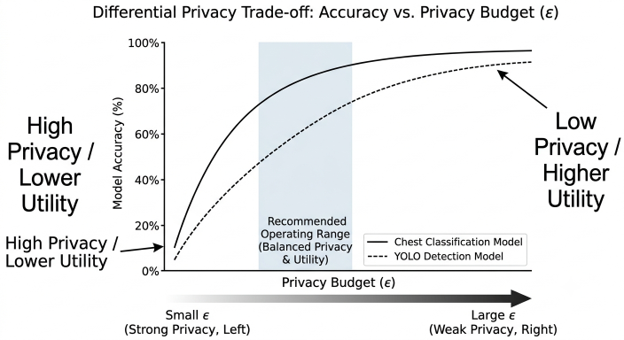
\includegraphics[width=0.8\textwidth]{assets/privacy_utility_tradeoff.png}
	\caption{Privacy--utility tradeoff under $(\epsilon,\delta)$-differential privacy. Smaller values of $\epsilon$ provide stronger privacy guarantees but may reduce model performance.}
	\label{fig:dp_tradeoff}
\end{figure}

\subsubsection{Additional Privacy Considerations}

Beyond gradient inversion attacks, model inversion and membership inference attacks represent additional privacy concerns.

Model inversion attempts to reconstruct representative training samples from a trained model, while membership inference seeks to determine whether a specific record was used during training.

Federated aggregation, large batch sizes, and differential privacy collectively reduce the effectiveness of these attack vectors.

\subsubsection{Transport-Layer Security (TLS)}

All model parameter exchanges are protected using mutual Transport Layer Security (mTLS) over gRPC.

The security infrastructure consists of:

\begin{itemize}
	\item Certificate Authority certificate (\texttt{ca.crt})
	\item Server certificate (\texttt{server.pem})
	\item Server private key (\texttt{server.key})
\end{itemize}

Mutual authentication ensures confidentiality, integrity, server authentication, and client authentication during communication.

In production deployments, TLS is mandatory and protects all federated learning traffic against interception and tampering.

\subsubsection{Authentication and Access Control}

Each participating institution receives a unique client identifier and API key during enrollment.

These credentials are required before client startup and are validated for every REST API request.

The authentication framework ensures:

\begin{itemize}
	\item Only authorized hospitals can participate.
	\item Unauthorized clients cannot submit updates.
	\item Client activity can be audited through server logs.
	\item Credentials remain external to source code repositories.
\end{itemize}

\subsubsection{Round Integrity and Liveness Controls}

The system continuously verifies round status before and during local training.

If a round is cancelled or completed, participating clients immediately terminate local computation and prevent obsolete updates from reaching the aggregation server.

Heartbeat messages are transmitted every fifteen seconds, enabling real-time monitoring of client availability and participation status.

These mechanisms improve both system integrity and operational reliability.

\subsubsection{Security Implementation Status Summary}

Table~\ref{tab:security_controls} summarizes the implementation status of all security controls incorporated into the federated learning platform.

\begin{table}[H]
	\centering
	\caption{Security Controls -- Implementation Status}
	\label{tab:security_controls}
	\renewcommand{\arraystretch}{1.2}
	\begin{tabularx}{\textwidth}{|p{3.8cm}|p{2cm}|p{1.8cm}|X|}
		\hline
		\textbf{Security Control} &
		\textbf{Category} &
		\textbf{Status} &
		\textbf{Notes} \\
		\hline
		
		Data locality (no raw data transmitted) &
		Privacy &
		Done &
		Core FL design property; only weight tensors transmitted \\
		\hline
		
		TLS encryption on gRPC channel &
		Transport &
		Done &
		\texttt{ca.crt} + \texttt{server.pem} + \texttt{server.key}; mutual TLS \\
		\hline
		
		API key authentication &
		Access Control &
		Done &
		\texttt{CLIENT\_API\_KEY} required; validated on every REST call \\
		\hline
		
		Client identity validation &
		Access Control &
		Done &
		\texttt{CLIENT\_ID} required; startup exit if absent \\
		\hline
		
		Large batch size ($B \geq 32$) &
		Privacy &
		Done &
		Mitigates gradient inversion attack fidelity \\
		\hline
		
		Heartbeat liveness monitoring &
		Integrity &
		Done &
		Continuous per-client liveness signal every 15 seconds \\
		\hline
		
		Per-epoch round-active check &
		Integrity &
		Done &
		Aborts training on cancelled round; covers both model types \\
		\hline
		
		Best-model checkpoint (local) &
		Robustness &
		Done &
		Restores best validation-loss weights before uploading to server \\
		\hline
		
		Selective YOLO federation (no head) &
		Integrity &
		Done &
		\texttt{cv3} detection head excluded from aggregation to prevent shape mismatch \\
		\hline
		
		Differential Privacy (DP noise) &
		Privacy &
		CONFIG-URABLE &
		Architecture supports $(\epsilon,\delta)$-DP; not yet enabled by default \\
		\hline
		
		Secure credential storage &
		Access Control &
		Done &
		\texttt{.env.template} pattern; credentials never stored in source code or container images \\
		\hline
		
		Shutdown-on-breach notification &
		Resilience &
		Done &
		Server sends \texttt{round-failed} webhook on unexpected shutdown \\
		\hline
		
	\end{tabularx}
\end{table}

The current implementation includes fully operational transport security, authentication, access control, liveness monitoring, and round integrity mechanisms. Differential privacy remains available as a configurable enhancement for deployments requiring stronger formal privacy guarantees.
\subsection{What Makes the Proposed System Distinctive}
\label{subsec:fl_novelty}
 
While federated learning has been applied in various medical imaging studies,
the majority of existing implementations are designed around a fixed model
architecture and a specific anatomical target, limiting their transferability
to new clinical tasks. The proposed framework differentiates itself through
the following design principles:
 
\textbf{Model Agnosticism.} The federated coordination layer — encompassing
client management, weight serialization, aggregation, and communication — is
fully decoupled from the local model definition. Any differentiable model
that can be expressed as a parameter vector (e.g., CNNs for classification,
U-Net variants for segmentation, Vision Transformers) can be substituted as
the local model without modifying the federated infrastructure. This makes
the system immediately applicable to new imaging tasks simply by swapping the
model definition on the client side.
  
\textbf{Staged Data Integration.} The system incorporates a staged data
feeding protocol that progressively increases each client's active training
subset across federated rounds. This design reflects the clinical reality
that expert-annotated medical imaging datasets grow incrementally over time
as radiologists label new cases. Rather than requiring a fully annotated
dataset before training begins, the system accommodates continuous data
growth, enabling earlier model deployment and iterative improvement as
annotation progresses.
 
\textbf{Containerized Reproducibility.} Each participating node is deployed
as an isolated Docker container, ensuring that the federated environment is
fully reproducible across different hardware configurations and operating
systems. The container-based architecture also simplifies scaling: adding a
new institution requires only the deployment of an additional client
container with the appropriate data volume mount, with no changes to the
server or existing clients.
 
\textbf{Framework Choice.} The system is implemented using the Flower
(flwr) framework~\cite{beutel2022}, selected for its support of multiple
ML backends (PyTorch, TensorFlow, JAX), its clean abstraction of the
client-server protocol, and its active development for healthcare FL
research. The backend-agnostic design of Flower further reinforces the
model-agnostic objective of the proposed system.
 
Collectively, these properties position the proposed FL framework as a
general-purpose infrastructure for privacy-preserving collaborative medical
image analysis, extensible to a wide range of clinical specialties and
diagnostic tasks without architectural redesign.


\section{Retrieval-Augmented Generation (RAG) Model}

The proposed platform incorporates a Retrieval-Augmented Generation (RAG) model to provide an intelligent medical question-answering assistant capable of responding to user inquiries using trusted medical knowledge sources. Unlike conventional large language models that rely solely on their internal parametric knowledge, the RAG approach augments the language model with information retrieved from an external knowledge base at inference time. This enables the system to generate responses that are more accurate, context-aware, explainable, and grounded in domain-specific medical information.

The primary objective of integrating the RAG model within the proposed framework is to provide users with a reliable conversational assistant capable of answering questions related to chest diseases, lung cancer, medical imaging, diagnostic procedures, and other healthcare-related topics. By retrieving relevant information from curated medical documents before response generation, the system significantly reduces hallucinations and improves the factual consistency of generated answers.

\subsection{Motivation}

Although modern Large Language Models (LLMs) demonstrate remarkable natural language understanding and generation capabilities, they suffer from several limitations when deployed in healthcare environments. Most notably, they may generate inaccurate information, provide outdated medical recommendations, or produce responses unsupported by clinical evidence.

In medical applications, such limitations can negatively affect user trust and potentially lead to harmful outcomes. Consequently, relying solely on the internal knowledge of a pretrained language model is insufficient for healthcare-oriented systems.

Retrieval-Augmented Generation addresses these challenges by combining information retrieval techniques with generative language models. Instead of answering questions exclusively from learned parameters, the system first retrieves relevant medical knowledge from an external document repository and then uses this information to guide response generation. This approach ensures that answers remain grounded in verified sources while maintaining the conversational capabilities of modern language models.

\subsection{Overview of the Proposed RAG Architecture}

The implemented RAG system consists of four major components:

\begin{enumerate}
	\item Medical Knowledge Base
	\item FAISS Vector Database
	\item Ollama Large Language Model
	\item LangChain Orchestration Layer
\end{enumerate}

The interaction between these components is illustrated in Figure~\ref{fig:rag_architecture}.

\begin{figure}[htbp]
	\centering
	
	\resizebox{\linewidth}{!}{
		\begin{tabular}{c c c c c c c c c}
			
			\fbox{
				\begin{tabular}{c}
					User\\
					Query
				\end{tabular}
			}
			
			&
			$\rightarrow$
			&
			
			\fbox{
				\begin{tabular}{c}
					Query\\
					Processing
				\end{tabular}
			}
			
			&
			$\rightarrow$
			&
			
			\fbox{
				\begin{tabular}{c}
					Embedding\\
					Generation
				\end{tabular}
			}
			
			&
			$\rightarrow$
			&
			
			\fbox{
				\begin{tabular}{c}
					FAISS\\
					Vector Search
				\end{tabular}
			}
			
			&
			$\rightarrow$
			&
			
			\fbox{
				\begin{tabular}{c}
					Relevant\\
					Document Chunks
				\end{tabular}
			}
			
		\end{tabular}
	}
	
	\vspace{0.6cm}
	
	$\downarrow$
	
	\vspace{0.4cm}
	
	\resizebox{0.8\linewidth}{!}{
		\begin{tabular}{c c c c c}
			
			\fbox{
				\begin{tabular}{c}
					Context\\
					Construction
				\end{tabular}
			}
			
			&
			$\rightarrow$
			&
			
			\fbox{
				\begin{tabular}{c}
					Qwen 2.5\\
					(LLM)
				\end{tabular}
			}
			
			&
			$\rightarrow$
			&
			
			\fbox{
				\begin{tabular}{c}
					Response\\
					Generation
				\end{tabular}
			}
			
		\end{tabular}
	}
	
	\vspace{0.6cm}
	
	$\downarrow$
	
	\vspace{0.4cm}
	
	\fbox{
		\begin{minipage}{0.45\linewidth}
			\centering
			Final Response + Source References
		\end{minipage}
	}
	
	\caption{Overall architecture of the proposed Retrieval-Augmented Generation (RAG) model. The user query is transformed into vector embeddings, relevant medical knowledge is retrieved from the FAISS vector database, and the retrieved context is supplied to the Qwen 2.5 language model to generate a grounded and source-aware response.}
	\label{fig:rag_architecture}
\end{figure}

The architecture begins when a user submits a natural language query through the platform interface. The query is forwarded to the FastAPI model backend, where LangChain orchestrates the retrieval and generation pipeline. Relevant document chunks are retrieved from the FAISS vector database and supplied as contextual information to the language model. The generated answer is then returned to the user along with references to the retrieved sources.

\subsection{Knowledge Base Construction}

The foundation of the RAG system is a curated collection of medical documents covering topics related to:

\begin{itemize}
	\item Chest diseases
	\item Pneumonia
	\item Tuberculosis
	\item COVID-19
	\item Lung cancer
	\item Medical imaging
	\item Diagnostic procedures
	\item Healthcare guidelines
\end{itemize}

These documents are converted into machine-processable representations before being indexed. Since language models cannot efficiently search through large collections of raw documents during inference, each document is divided into smaller semantic chunks.

Chunking improves retrieval accuracy by allowing the system to retrieve only the most relevant portions of a document rather than entire files.

For each generated chunk, metadata is preserved, including:

\begin{itemize}
	\item Document name
	\item Page number
	\item Source identifier
	\item Document category
\end{itemize}

This metadata later enables source attribution and transparency within generated responses.

\subsection{Vector Embedding Generation}

After document chunking, each text segment is transformed into a dense numerical representation known as an embedding vector.

Embeddings encode semantic meaning into a high-dimensional vector space, allowing documents with similar meanings to be located near one another mathematically.

Given a document chunk $(d\_i)$, an embedding function (E($\cdot$)) produces a vector representation $v_i = E(d_i)$ 
where $v_i \in \mathbb{R}^{n}$ and $(n)$ represents the embedding dimensionality.

These embeddings capture semantic relationships between medical concepts and enable similarity-based retrieval during inference.

\subsection{FAISS Vector Database}

To support efficient retrieval over thousands of embedded document chunks, the system employs Facebook AI Similarity Search (FAISS).

FAISS is a high-performance vector database specifically designed for similarity search within large embedding collections. Instead of performing keyword matching, FAISS retrieves documents based on semantic similarity.

All generated embeddings are stored within the FAISS index.

During inference, a user query is embedded using the same embedding model: $q = E(x)$ where $(x)$ denotes the user's query.

The FAISS index then searches for the (k) nearest vectors according to cosine similarity and returns the most relevant document chunks.

This retrieval process allows the system to locate contextually relevant medical information even when the exact wording differs from that found in the original documents.

\subsection{Large Language Model Integration}

The generative component of the RAG pipeline utilizes the Qwen 2.5 language model deployed locally through Ollama.

Running the model locally provides several advantages:

\begin{itemize}
	\item Reduced operational cost
	\item Improved privacy
	\item Low latency
	\item Full deployment control
	\item Offline inference capability
\end{itemize}

The model configuration used in the implementation is summarized in Table~\ref{tab:rag_model_configuration}.

\begin{table}[htbp]
	\centering
	\caption{Configuration of the deployed language model.}
	\label{tab:rag_model_configuration}
	\begin{tabular}{|l|l|}
		\hline
		\textbf{Parameter} & \textbf{Value} \\ 
		\hline
		LLM Engine & Ollama \\
		\hline
		Model & qwen2.5:3b \\
		\hline
		Temperature & 0.5 \\
		\hline
		Max Tokens & 500 \\
		\hline
		Keep Alive & Infinite (-1) \\
		\hline
	\end{tabular}
\end{table}

After retrieval, the selected document chunks are appended to the prompt supplied to the language model. Consequently, generated responses become grounded in retrieved medical knowledge rather than relying exclusively on pretrained parameters.

\subsection{Query Processing Workflow}

The complete RAG workflow implemented within the system is illustrated in Figure~\ref{fig:rag_workflow}.

\begin{figure}[htbp]
	\centering
	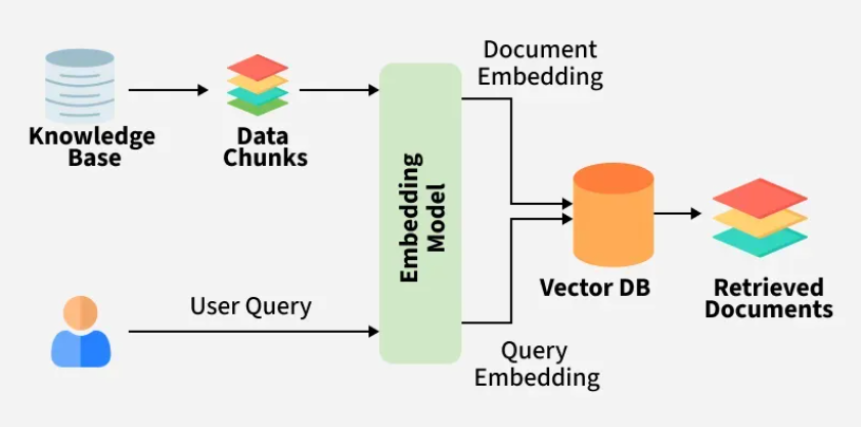
\includegraphics[width=\linewidth]{assets/RAG_1.png}
	\caption{Query processing workflow of the proposed RAG system.}
	\label{fig:rag_workflow}
\end{figure}

The workflow consists of the following steps:

\begin{enumerate}
	\item User submits a medical question.
	\item Query is forwarded to the FastAPI backend.
	\item Query embedding is generated.
	\item FAISS retrieves the most relevant document chunks.
	\item Retrieved context is assembled.
	\item Context and user query are passed to Qwen 2.5.
	\item The language model generates a grounded response.
	\item Source metadata is attached.
	\item Final response is returned to the user.
\end{enumerate}

\subsection{Source Attribution and Explainability}

One of the most important characteristics of the proposed RAG implementation is transparency.

Rather than generating answers without justification, the system preserves metadata associated with retrieved documents and returns source references alongside generated responses. This allows users to trace the origin of information and verify the supporting evidence used during answer generation. The underlying report emphasizes that retrieved documents and page references are preserved to improve transparency and user trust.

Providing source-aware responses is particularly important in healthcare applications where explainability and evidence-based recommendations are essential.

\subsection{Advantages of the Proposed Approach}

The implemented Retrieval-Augmented Generation model provides several advantages:

\begin{itemize}
	\item Reduces hallucinations compared with standalone LLMs.
	\item Produces responses grounded in medical knowledge sources.
	\item Supports explainable and source-aware answers.
	\item Enables efficient retrieval through FAISS vector search.
	\item Preserves privacy through local deployment using Ollama.
	\item Can be continuously expanded by adding new medical documents.
	\item Integrates seamlessly with the overall X-Fed Neuroscan architecture.
\end{itemize}

Consequently, the RAG subsystem serves as an intelligent medical assistant that complements the image analysis capabilities of the platform by providing users with reliable, contextualized, and explainable healthcare information.


\section{Platform Architecture}
The system  is a comprehensive web-based healthcare management system developed to streamline medical services and enhance diagnostic workflows through an integrated digital platform. The system provides a centralized environment where patients, doctors, administrators, and healthcare institutions can interact efficiently through role-based dashboards and specialized services.
The platform allows patients to create accounts, manage their profiles, book appointments, track medical records, and communicate through an intelligent healthcare assistant. Doctors can manage appointments, analyze medical images, review patient information, and assign diagnostic results, while administrators oversee user management, system operations, and hospital coordination. The system also supports healthcare institutions participating in collaborative AI model development through federated learning mechanisms.
Built using a modern multi-tier architecture, XFed NeuroScan combines a responsive web interface, secure backend services, cloud-based storage, and artificial intelligence modules to deliver a seamless user experience. The application emphasizes security, scalability, and usability by implementing role-based access control, secure authentication, real-time communication, and centralized healthcare workflows.
By integrating healthcare management features with intelligent diagnostic services, XFed NeuroScan provides a unified platform that improves operational efficiency, supports medical decision-making, and enhances the overall experience for both healthcare providers and patients.

The platform is composed of four tightly integrated repositories:
\begin{itemize}
	\item \textbf{Frontend:} React 18 single-pages application serving doctors, patients, and administrators.
	\item \textbf{Backend:} Spring Boot 3.5 REST and WebSocket API acting as the central system of record, handling authentication, business logic, user management, and communication between services.
	\item \textbf{Model Backend:} FastAPI-based AI service responsible for medical image analysis, chest disease classification, lung cancer detection, explainable AI heatmap generation, and a Retrieval-Augmented Generation (RAG) medical chatbot for intelligent question answering.
	\item \textbf{Federated-Learning Server:} Flower-based federated learning coordinator managing hospital registration, client monitoring, distributed training rounds, and global model aggregation.
\end{itemize} 
Together, these components provide a complete healthcare platform that combines medical workflow management, AI-assisted diagnosis, intelligent medical assistance through RAG, and privacy-preserving federated learning across multiple healthcare institutions.

\begin{table}[htbp]
	\centering
	\caption{Summary of the proposed X-Fed NeuroScan framework.}
	\label{tab:framework_summary}
	\begin{tabular}{|p{4cm}|p{9cm}|}
		\hline
		\textbf{Dimension} & \textbf{Detail} \\
		\hline
		Primary Domain & Medical imaging and AI-based diagnostic systems \\
		\hline
		Key Innovation & Federated learning for privacy-preserving model improvement and collaborative model training across institutions \\
		\hline
		User Roles & Patient, Doctor, and Administrator \\
		\hline
		Imaging Modalities & Chest X-ray classification (COVID-19, Tuberculosis, Pneumonia, and Normal) and lung cancer detection from CT scans \\
		\hline
		AI Explainability & Grad-CAM heatmaps for chest disease predictions and lesion localization visualizations for lung cancer detection \\
		\hline
		Privacy Model & Raw medical images never leave hospital premises; only model parameters are exchanged during federated learning \\
		\hline
	\end{tabular}
\end{table}

\subsection{End-to-End System Architecture}The system follows a microservices architecture. Four independent services communicate over well-defined APIs. The frontend is the only entry point for human users; all backend services are internal.

\subsubsection{Service Map}
Table~\ref{tab:system_components} lists all the different components and services of the proposed system.
\begin{table}[htbp]
	\centering
	\caption{Technological components of the proposed system architecture.}
	\label{tab:system_components}
	\begin{tabular}{|p{3.5cm}|p{4.5cm}|p{2cm}|p{5cm}|}
		\hline
		\textbf{Service} & \textbf{Technology} & \textbf{Port} & \textbf{Primary Role} \\
		\hline
		Frontend &
		React 18, Vite, and TypeScript &
		3000 &
		User interface for patients, doctors, and administrators \\
		\hline
		
		Backend &
		Spring Boot 3.5 and Java 21 &
		8080 &
		Authentication, business logic implementation, and API gateway services \\
		\hline
		
		Model Backend &
		FastAPI and Python 3 &
		8000 &
		Machine learning inference services and retrieval-augmented generation (RAG) chatbot functionality \\
		\hline
		
		Federated Learning Server &
		FastAPI, Flower, and Python 3 &
		8001 / 50051 &
		Federated learning coordination, client management, and hospital registry services \\
		\hline
	\end{tabular}
\end{table}

\subsubsection{External Infrastructure}
During system implementation, we  have also relied on external components to not reinvent the wheel  and leverage already existing powerful and free infrastructure, those components are listed in Table~\ref{tab:supporting_infrastructure}
\begin{table}[htbp]
	\centering
	\caption{Supporting infrastructure and external services used by the proposed system.}
	\label{tab:supporting_infrastructure}
	\begin{tabular}{|p{4.5cm}|p{10cm}|}
		\hline
		\textbf{Component} & \textbf{Role} \\
		\hline
		
		Cloudflare R2 (S3-Compatible Storage) &
		Stores uploaded medical images, generated Grad-CAM heatmaps, lung cancer detection result overlays, and other imaging-related artifacts. \\
		\hline
		
		PostgreSQL &
		Primary relational database used to manage users, medical images, appointments, hospital information, federated learning participants, and other persistent application data. \\
		\hline
		
		Redis &
		Provides high-speed storage for refresh tokens and caching of presigned URLs to improve system performance and reduce unnecessary storage requests. \\
		\hline
		
		Ollama (qwen2.5:3b) &
		Local large language model (LLM) responsible for generating responses within the retrieval-augmented generation (RAG) chatbot component. \\
		\hline
		
		Gmail SMTP &
		Handles transactional email services including password reset requests, user invitations, account notifications, and hospital package communications. \\
		\hline
		
		FAISS &
		Vector similarity search engine used to index and retrieve relevant documents for the retrieval-augmented generation (RAG) pipeline. \\
		\hline
		
	\end{tabular}
\end{table}

\subsubsection{Architecture Visualization}

To provide a clearer understanding of the overall system structure, Figures~\ref{fig:system_architecture_overview} and \ref{fig:deployment_architecture_overview} present visual representations of the proposed \textit{X-Fed NeuroScan} framework. These diagrams complement the architectural descriptions presented throughout this chapter by illustrating the interaction between system components, data flow pathways, and deployment services. Together, they provide a comprehensive view of both the logical architecture of the framework and the technological infrastructure used to support its operation.

\begin{figure}[htbp]
	\centering
	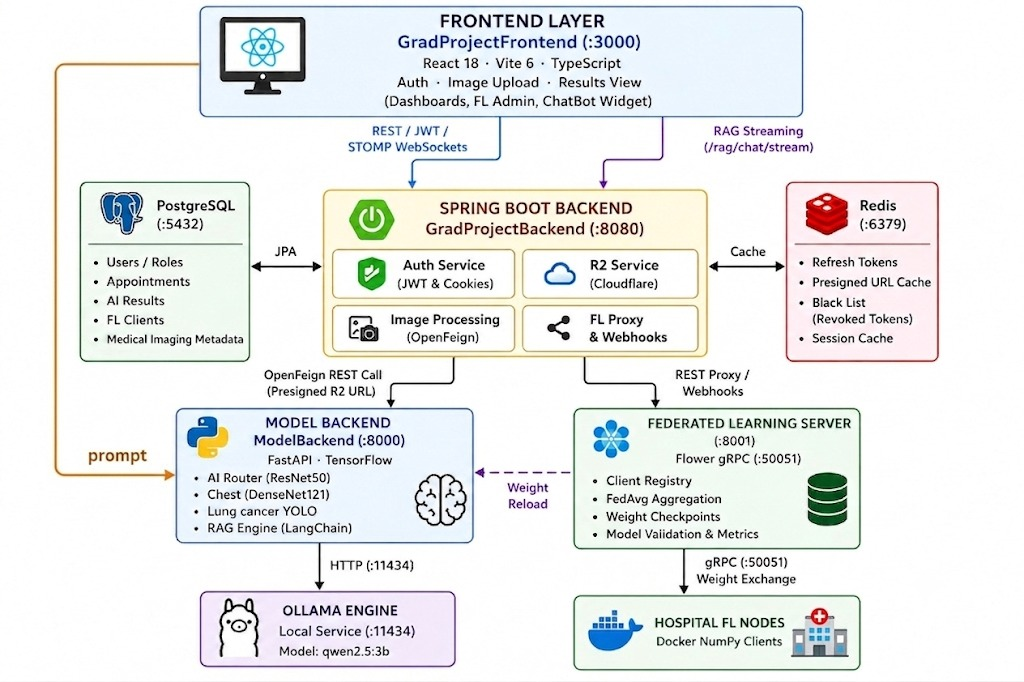
\includegraphics[width=0.95\linewidth]{assets/backend-1-ag.jpeg}
	\caption{End-to-end logical architecture of the proposed X-Fed NeuroScan framework, illustrating the interaction between users, backend services, AI models, explainability components, federated learning infrastructure, and data storage systems.}
	\label{fig:system_architecture_overview}
\end{figure}

\begin{figure}[htbp]
	\centering
	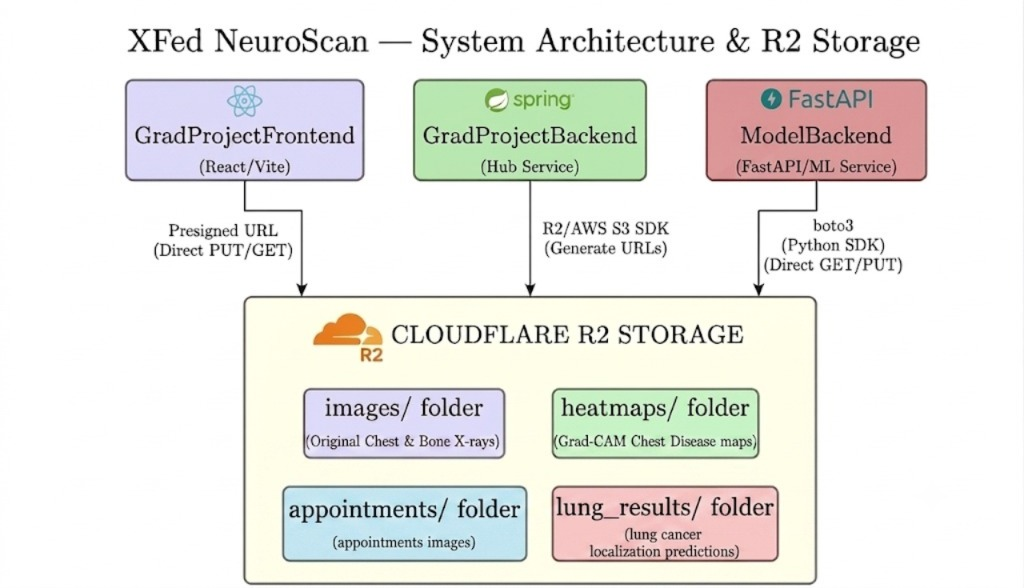
\includegraphics[width=0.95\linewidth]{assets/backend-2-ag.jpeg}
	\caption{Deployment architecture of the proposed system showing the frontend application, backend services, model-serving infrastructure, federated learning server, databases, storage components, and external integrations.}
	\label{fig:deployment_architecture_overview}
\end{figure}

\subsection{Frontend}
The frontend is a React 18 single-page application built with Vite 6 and TypeScript. It serves three user roles — Patient, Doctor, and Admin — through role-gated dashboards, and is the sole human interface into the platform.

\subsubsection{Technology Stack}
Different technologies were used during the development and implementation of the frontend components of the proposed system. They have been listed in Table~\ref{tab:frontend_technologies}.
\begin{table}[htbp]
	\centering
	\caption{Frontend technologies used in the implementation of the proposed system.}
	\label{tab:frontend_technologies}
	\begin{tabular}{|p{4cm}|p{8.5cm}|}
		\hline
		\textbf{Category} & \textbf{Technology} \\
		\hline
		
		Framework &
		React 18 \\
		\hline
		
		Build Tool &
		Vite 6 with \texttt{@vitejs/plugin-react-swc} \\
		\hline
		
		Programming Language &
		TypeScript 5 (Strict Mode) \\
		\hline
		
		Routing &
		React Router 7 \\
		\hline
		
		Styling &
		Tailwind CSS v4 \\
		\hline
		
		UI Primitives &
		Radix UI with shadcn-style wrapper components \\
		\hline
		
		Animations &
		Framer Motion (Motion) \\
		\hline
		
		Charts and Data Visualization &
		Recharts \\
		\hline
		
		Real-Time Communication &
		\texttt{@stomp/stompjs} and \texttt{sockjs-client} \\
		\hline
		
		Form Management &
		react-hook-form \\
		\hline
		
	\end{tabular}
\end{table}

\subsubsection{User Roles \& Capabilities}
The system is designed as a role-based healthcare to ensure that each type of user interacts with the platform according to their responsibilities, permissions, and level of access. The system defines three main roles: Patient, Doctor, and Administrator, each serving a distinct purpose within the healthcare workflow.

Patients represent the end users of the system. Their role is limited to personal healthcare management, including registering accounts, booking appointments, viewing medical history, and accessing their own diagnostic results. This restricted access ensures that patients can interact with their healthcare data securely without modifying clinical or system-level information.

Doctors have a more advanced role focused on medical operations. They can upload and analyze medical images, review AI-generated predictions, interpret results, and assign diagnoses to patients. In addition, doctors manage appointments and clinical interactions with patients. This role requires broader access because it directly involves medical decision-making and the use of AI diagnostic tools.
Administrators hold the highest level of control within the system. They are responsible for managing users, including creating and inviting doctors, monitoring system activity, and overseeing hospital and federated learning operations. Administrators also handle system configuration and ensure that all services operate securely and efficiently.

The separation of roles is essential for maintaining security, privacy, and operational clarity. By limiting access based on responsibilities, the system prevents unauthorized actions, reduces the risk of data misuse, and ensures that each user interacts only with the features relevant to their function. This role-based design also improves usability by providing a tailored interface for each type of user, making the system more efficient and easier to navigate.

\begin{table}[htbp]
	\centering
	\caption{User roles and capabilities within the proposed X-Fed NeuroScan system.}
	\label{tab:user_roles_capabilities}
	\begin{tabular}{|p{3cm}|p{9.5cm}|}
		\hline
		\textbf{Role} & \textbf{Capabilities} \\
		\hline
		
		Patient &
		View personalized dashboard statistics, book appointments with doctors, upload medical image attachments, access diagnostic results, and review prediction history. \\
		\hline
		
		Doctor &
		Analyze chest medical images using the integrated AI models, assign diagnostic results to patients, manage appointment schedules, review patient records, and access prediction history. \\
		\hline
		
		Administrator &
		Perform full platform administration including user management, federated learning hospital registration, hospital selection for federated training rounds, monitoring system activity, and conducting image analysis through the integrated diagnostic framework. \\
		\hline
		
	\end{tabular}
\end{table}

\subsubsection{Key Pages and Routing}
Frontend is structured as a single-page application with role-based routing to ensure secure and organized access to system features. Each user type is directed to specific pages depending on their permissions and responsibilities within the platform.

Public users can access the landing page and authentication-related pages, including login, signup, password recovery, and invite-based account activation. These pages are only available to guests who are not yet authenticated.

Authenticated users are redirected to role-specific dashboards after login. Patients have access to their personal dashboard and medical history, where they can view appointments and diagnostic results. Doctors are provided with a dedicated dashboard along with access to image analysis tools and patient-related medical data. Administrators have the highest level of access, allowing them to manage users, monitor system activity, and control federated learning operations.

In addition to dashboards, administrators also access specialized modules for user management and federated learning configuration, including hospital registration and training round setup. The image analysis page is restricted to doctors and administrators due to its clinical importance and use of AI-based diagnostic tools.

Overall, the routing structure enforces strict role-based access control, ensuring that each user interacts only with the features relevant to their responsibilities while maintaining system security and usability.

\begin{table}[htbp]
	\centering
	\caption{Access control policy for system pages and administrative modules.}
	\label{tab:system_page_access_control}
	\begin{tabular}{|p{4cm}|p{6.5cm}|}
		\hline
		\textbf{Page} & \textbf{Access} \\
		\hline
		
		Landing Page &
		Publicly accessible to all users, including unauthenticated visitors. \\
		\hline
		
		Authentication Pages &
		Accessible only to guest users who have not yet authenticated. \\
		\hline
		
		Password Recovery &
		Accessible only to guest users initiating the password reset process. \\
		\hline
		
		Invite Activation &
		Accessible only through a valid invitation token provided to the invited user. \\
		\hline
		
		Image Analysis &
		Accessible to users with Administrator or Doctor privileges. \\
		\hline
		
		Prediction History &
		Accessible to Administrators, Doctors, and Patients according to their authorization level. \\
		\hline
		
		Administrator Dashboard &
		Accessible exclusively to users with the Administrator role. \\
		\hline
		
		Doctor Dashboard &
		Accessible exclusively to users with the Doctor role. \\
		\hline
		
		Patient Dashboard &
		Accessible exclusively to users with the Patient role. \\
		\hline
		
		User Management &
		Accessible exclusively to Administrators for managing user accounts and permissions. \\
		\hline
		
		Federated Learning Hospital Management &
		Accessible exclusively to Administrators for registering, updating, and monitoring participating hospitals. \\
		\hline
		
		Federated Learning Training Round Setup &
		Accessible exclusively to Administrators for configuring and launching federated learning training rounds. \\
		\hline
		
	\end{tabular}
\end{table}

\subsubsection{Core Features}
\paragraph{Authentication \& Session Management}
The frontend implements a full authentication lifecycle using JWT access tokens are stored in memory (not localStorage); refresh tokens are stored in HttpOnly cookies. On app load, the context attempts a silent token refresh to restore sessions without requiring re-login. GuestRoute prevents authenticated users from visiting auth. pages; Require Dashboard Role guards all dashboard routes.

\paragraph{Medical Image Analysis}
The image analysis flow uses a presigned-URL pattern to avoid routing large files through the backend:
\begin{itemize}
	\item Step 1: Frontend requests a presigned R2 PUT URL from Spring Backend 
	\item Step 2: Frontend uploads the image directly to Cloudflare R2
	\item Step 3: Frontend calls the api who is responsible for image-processing with the R2 key
	\item Step 4: Backend triggers Model inference and returns prediction, confidence, and heatmap URL
\end{itemize}

\paragraph{Federated Learning Management}
Admins manage FL hospitals through two dedicated pages. FLHospitalsPage shows all registered hospital nodes with live ONLINE/OFFLINE status via WebSocket. FL Select Hospitals Page lets admins choose which hospitals participate in the next training round. Registration generates an API key displayed once via ApiKeySuccessDialog.

\paragraph{AI Chatbot (RAG)}
A floating chat widget  is available on every page. Responses are streamed from the RAG service. The chatbot gracefully degrades to keyword-based mock answers if the RAG API is unreachable.

\begin{figure}[htbp]
	\centering
	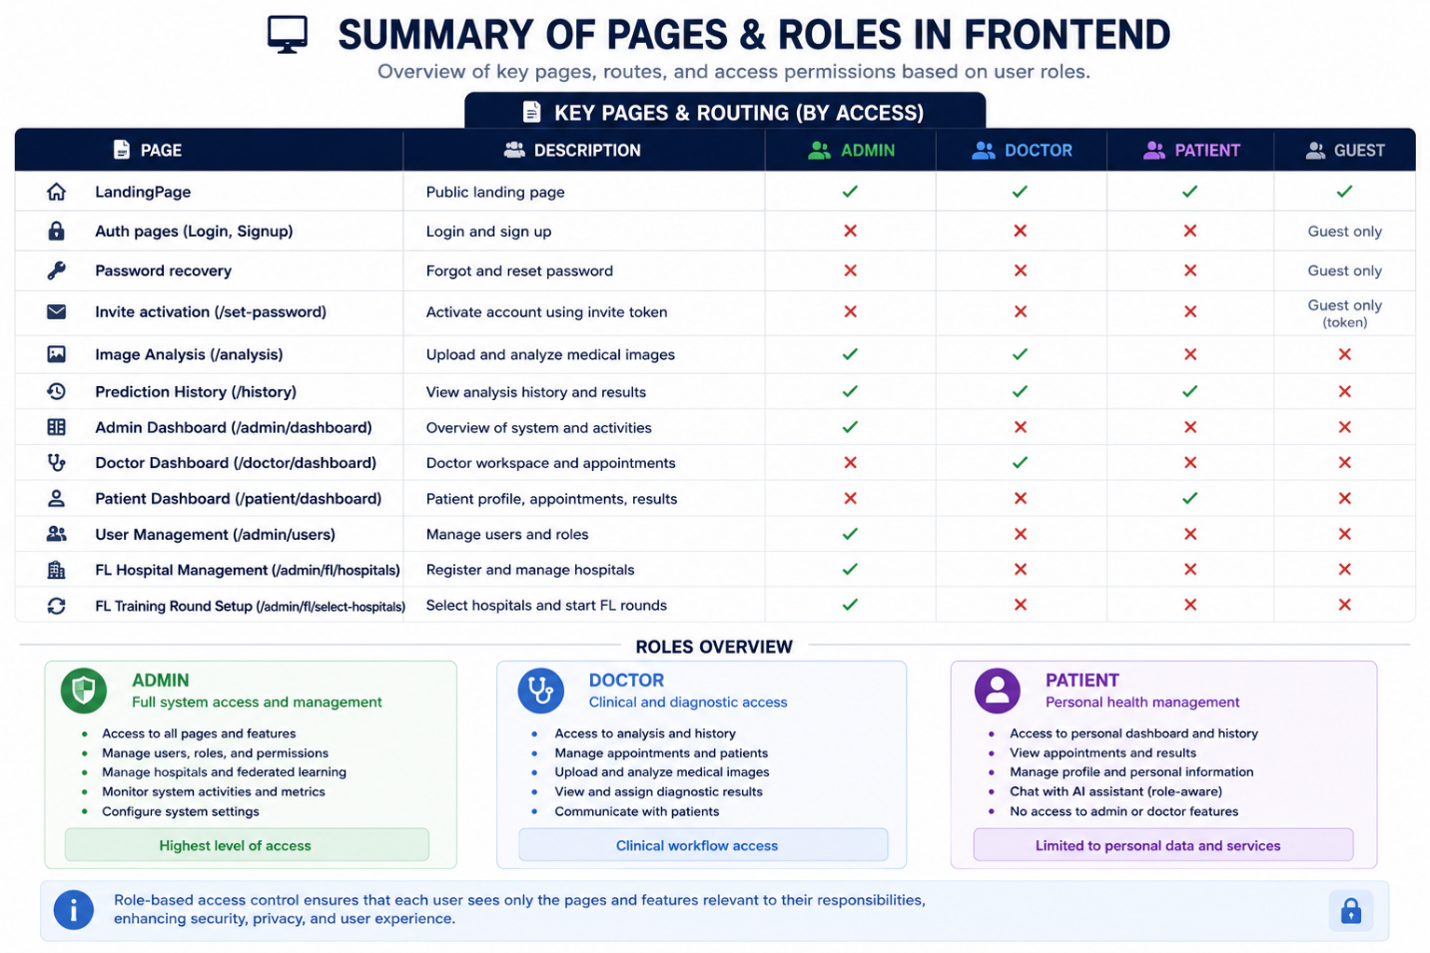
\includegraphics[width=0.95\linewidth]{assets/backend3.png}
	\caption{A visualization of the roles and pages implemented in the web application.}
	\label{fig:roles_pages_summary}
\end{figure}

\subsection{Centralized Backend (Spring Boot)}
Centralized backend is a Spring Boot 3.5 application written in Java 21. It serves as the central API gateway and system of record for authentication, user management, medical image orchestration, appointments, federated learning coordination, and real-time WebSocket broadcasts. 

\subsubsection{Technology Stack}
Various technologies were utilized in the implementation of the backend of the proposed end-to-end system. All of these technologies are listed in Table~\ref{tab:backend_technologies}.
\begin{table}[htbp]
	\centering
	\caption{Backend technologies used in the implementation of the proposed system.}
	\label{tab:backend_technologies}
	\begin{tabular}{|p{4cm}|p{8.5cm}|}
		\hline
		\textbf{Category} & \textbf{Technology} \\
		\hline
		
		Framework &
		Spring Boot 3.5.4 \\
		\hline
		
		Programming Language &
		Java 21 \\
		\hline
		
		Build Tool &
		Maven \\
		\hline
		
		Security &
		Spring Security 6 with JSON Web Token (JWT) authentication using JJWT 0.12.3 \\
		\hline
		
		Persistence Layer &
		Spring Data JPA, Hibernate, and PostgreSQL \\
		\hline
		
		Cache and Session Management &
		Spring Data Redis \\
		\hline
		
		HTTP Client &
		Spring Cloud OpenFeign \\
		\hline
		
		Real-Time Communication &
		Spring WebSocket, STOMP, and SockJS \\
		\hline
		
		Object Storage Integration &
		AWS SDK v2 for S3-compatible storage (Cloudflare R2) \\
		\hline
		
		Email Services &
		Spring Mail with Gmail SMTP \\
		\hline
		
		API Documentation &
		SpringDoc OpenAPI (Swagger UI) \\
		\hline
		
		Object Mapping and Code Generation &
		MapStruct and Lombok \\
		\hline
		
	\end{tabular}
\end{table}

\subsubsection{Security \& Authentication}

\begin{figure}[htbp]
	\centering
	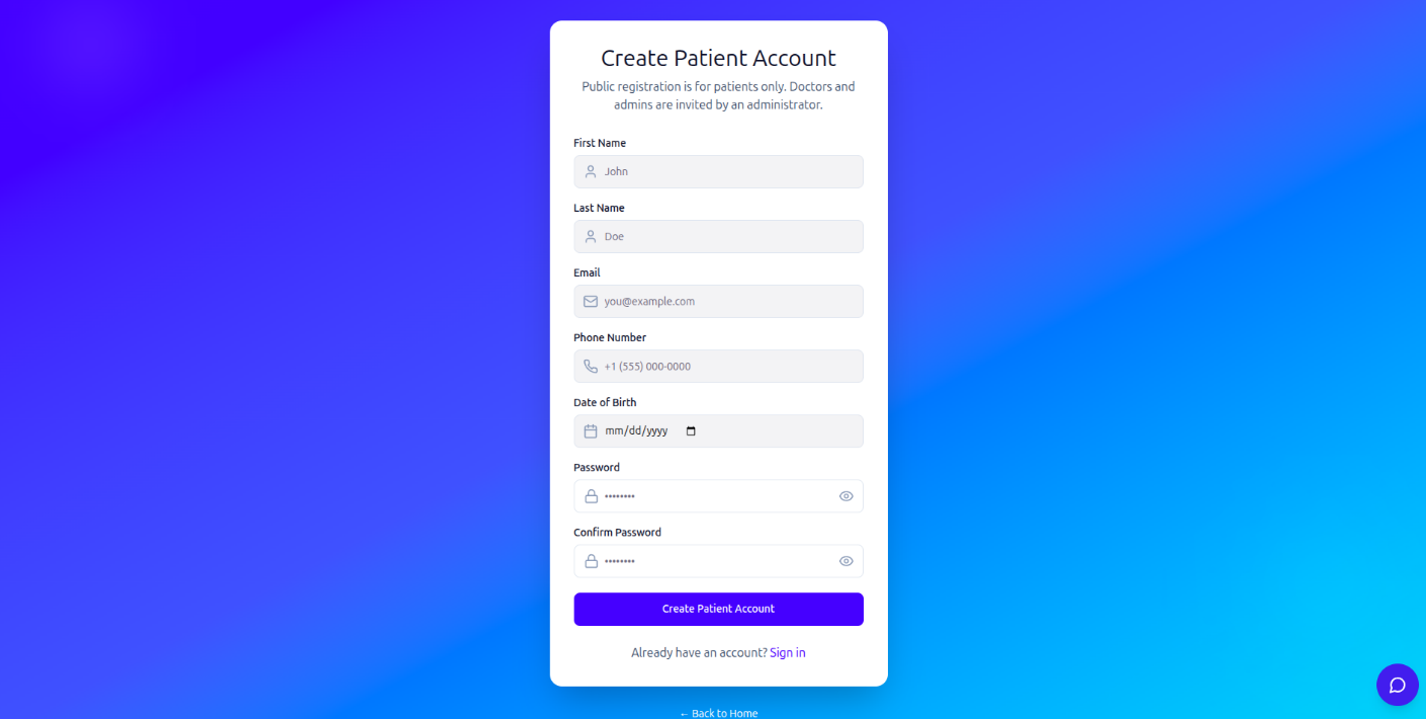
\includegraphics{assets/backend4.png}
	\caption{An image of the Create Account interaction from the web application.}
	\label{fig:create_account}
\end{figure}

\begin{figure}[htbp]
	\centering
	
\includegraphics{assets/backend5.png}
	\caption{An image of the Login interaction from the web application.}
	\label{fig:login}
\end{figure}

Security is implemented with JWT access tokens and HttpOnly refresh-token cookies stored in Redis:
\begin{itemize}
	\item Access Tokens: short-lived JWTs returned in the login response body
	\item Refresh Tokens: longer-lived tokens stored in Redis (key: email:deviceId) and set as HttpOnly cookies
	\item Logout: access tokens blacklisted when still valid; refresh token deleted from Redis
	\item FL API keys: encrypted at rest using AES via EncryptionUtils
	\item FL webhook endpoints: authenticated with a shared secret (not JWT)
	\item Soft delete: deleted users cannot log in
\end{itemize}

In the current system design, \textbf{login is restricted to patients only}. Doctor and Admin accounts are not self-authenticated through public signup; instead, they are created and managed exclusively by an administrator and activated through an invitation-based workflow. This ensures strict control over privileged roles in the healthcare system.

After login, user information is stored in PostgreSQL, but sensitive session data is handled separately for security. Passwords are never stored in plain text; instead, they are hashed using \textbf{BCrypt} before being saved in the database, making them irreversible and protected even if the database is compromised.

During authentication, the input password is hashed and compared with the stored hash. If valid, the system generates a short-lived \textbf{JWT access token} and a long-lived \textbf{refresh token}. The access token is used for API requests, while the refresh token is stored securely in \textbf{Redis} and also set as an \textbf{HttpOnly cookie}.

When the user logs out, the access token is blacklisted and the refresh token is removed from Redis, fully terminating the session. This design ensures secure password storage, stateless authentication, and strong session protection. 

In the system, only Admin users have the authority to create or manage Doctor and other Admin accounts, ensuring strict role control and preventing unauthorized privilege escalation.

New privileged users (Doctors or Admins) cannot register through the public signup process. Instead, an Admin must explicitly create or invite them through the administrative interface. This invitation-based flow allows the system to maintain tight control over sensitive roles that have access to clinical data, AI analysis tools, and system-wide management features.

\begin{figure}[htbp]
	\centering
	
\includegraphics{assets/backend6.png}
	\caption{An image of the Add User interaction from the web application.}
	\label{fig:add_user}
\end{figure}

After an Admin creates a new Doctor or Admin account, the account does not become active immediately. Instead, it enters a pending state until it is explicitly approved. This approval step ensures that no privileged user gains access to the system without proper verification and administrative confirmation.

During this pending phase, the user record is already stored in the database, but the account remains inactive, meaning the user cannot log in or access any system features. Once the Admin approves the account, its status is updated to active, and the user is then able to authenticate and use the system according to their assigned role.

In the user management interface, the Admin has full control over viewing and organizing all system users through a role-based filtering system. This allows the Admin to efficiently manage large numbers of accounts by categorizing users according to their current role and status.

In addition to account creation and approval, the Admin also has full control over existing privileged accounts, as shown in \ref{fig:user_mgmt}. This includes the ability to disable or delete accounts at any time. Disabling an account temporarily prevents the user from logging in without removing their data, while deletion marks the account as removed (soft delete), ensuring it is excluded from authentication and system operations but still preserved for audit or historical purposes.

\begin{figure}[htbp]
	\centering
	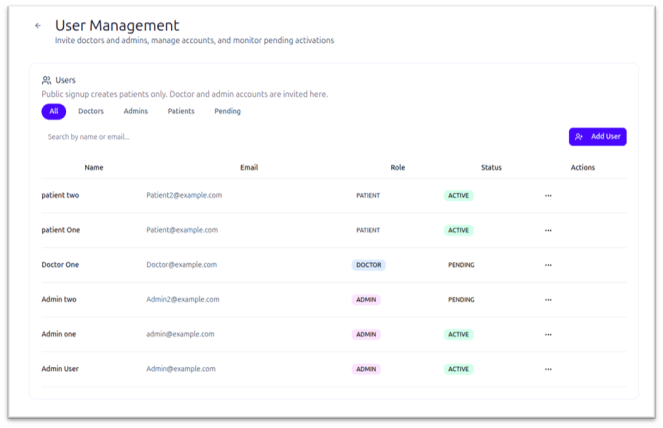
\includegraphics[width=0.95\linewidth]{assets/backend7.png}
	\caption{An image of the User Management tab from the web application.}
	\label{fig:user_mgmt}
\end{figure}

When a user selects “Forgot Password”, the system follows a secure multi-step flow to ensure that only the legitimate account owner can reset the password.

First, the user enters their registered email address in the frontend. This request is sent to the Spring Boot backend, which validates whether the email exists in the system. If the user is found, Spring Boot generates a secure password reset token, typically a short-lived, random token linked to the user account.

This token is then stored temporarily (or associated with the user record) and sent to the user via email using Gmail SMTP. The email contains a secure reset link that includes the token as a parameter.

When the user clicks the link, they are redirected to the password reset page in the frontend. The new password is submitted along with the token, and Spring Boot validates the token to ensure it is still valid and has not expired or been used before.

If the token is valid, the system hashes the new password using BCrypt and updates it in the PostgreSQL database, replacing the old password hash. After successful reset, the token is invalidated to prevent reuse.

Overall, the forgot password process ensures security by combining email verification, time-limited tokens, secure transmission, and encrypted password storage.

So in summary User authentication in system uses a secure JWT-based system where only patients can self-register and log in, while doctors and admins are created by admins. Passwords are stored in the database using BCrypt hashing.

After successful login, the system issues a short-lived JWT access token and a long-lived refresh token stored in Redis as an HttpOnly cookie. The access token is used for requests, and the refresh token allows session renewal.

The system also supports a secure forgot password workflow, where a password reset token is generated, sent to the user via email, and validated before allowing password updates. The new password is then hashed using BCrypt and stored in the database.

On logout, tokens are invalidated by blacklisting the access token and removing the refresh token. Role-based access control and soft delete ensure only authorized and active users can access the system.

\begin{figure}[htbp]
	\centering
	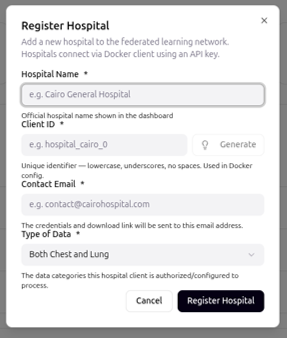
\includegraphics{assets/backend8.png}
	\caption{An image of the Add Hospital interaction from the web application.}
	\label{fig:add_hospital}
\end{figure}

\begin{figure}[htbp]
	\centering
	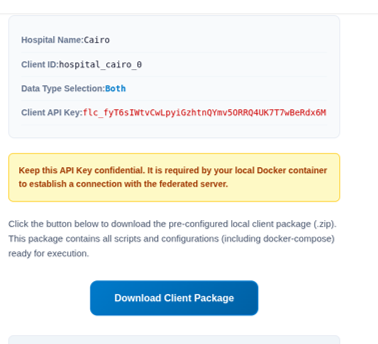
\includegraphics{assets/backend9.png}
	\caption{An image of the client hospital getting a confidential API key interaction from the web application.}
	\label{fig:hospital_api}
\end{figure}

Backend handles the full lifecycle of registering new hospitals in the federated learning system. When an Admin submits a hospital, Spring Boot validates the request, ensures only Admins can perform the action, and then generates a unique FL client ID and encrypted API key using AES before storing them in PostgreSQL. The hospital is initially saved with a PENDING or INACTIVE status.

After that, Spring Boot registers the hospital with the Federated Learning Server by sending its credentials and metadata, allowing it to join the federated learning network. It may also provide a Docker-based client package for hospital deployment.

Spring Boot receives and synchronizes key data from the Federated Learning (FL) Server, especially hospital online/offline status, which is determined by heartbeat signals sent from hospital clients to the FL Server. Spring Boot does not calculate this status itself; instead, it periodically fetches updated client information from the FL Server.

Overall, Spring Boot acts as a bridge that collects, stores, and distributes FL Server status updates, giving administrators a live view of the federated learning network.

When a new hospital is registered in the federated learning system, Spring Boot not only creates and stores the hospital record, but also sends an automated email notification via Gmail SMTP as part of the onboarding process.

After the Admin submits and approves the hospital registration, Spring Boot generates the hospital’s federated learning credentials (such as the FL client ID and encrypted API key) and securely stores them in the database. Once the registration is successfully completed, Spring Boot triggers the email service to notify the hospital.

This email is sent using Gmail SMTP integration and typically contains important onboarding information such as the hospital’s activation status, instructions for joining the federated learning network, and in some cases, a link or attachment for downloading the Docker-based FL client package required to connect to the FL server.

This step ensures that hospitals are immediately informed after registration and can proceed with setup and participation in federated learning without manual coordination. It also improves system automation and reduces administrative overhead while maintaining secure delivery of sensitive setup information.

\subsubsection{Medical Image Pipeline}
The backend orchestrates image analysis without storing raw images locally:
\begin{itemize}
	\item Presigned PUT URL is generated for direct R2 upload (5-minute expiry).
	\item After upload, backend saves image metadata to PostgreSQL
	\item ModelBackend is called via OpenFeign (Feign client) with a presigned GET URL
	\item ML results — prediction label, confidence score, heatmap S3 key — are persisted
	\item Presigned GET URLs for original and heatmap images are cached in Redis (~59 min TTL)
\end{itemize}

Small parts of the pipeline can be shown in \ref{fig:greeting_}, and \ref{fig:greeting_2} where the user is asked to upload a medical image to the system so that they are directed to the right models and diagnosed.

\begin{figure}[htbp]
	\centering
	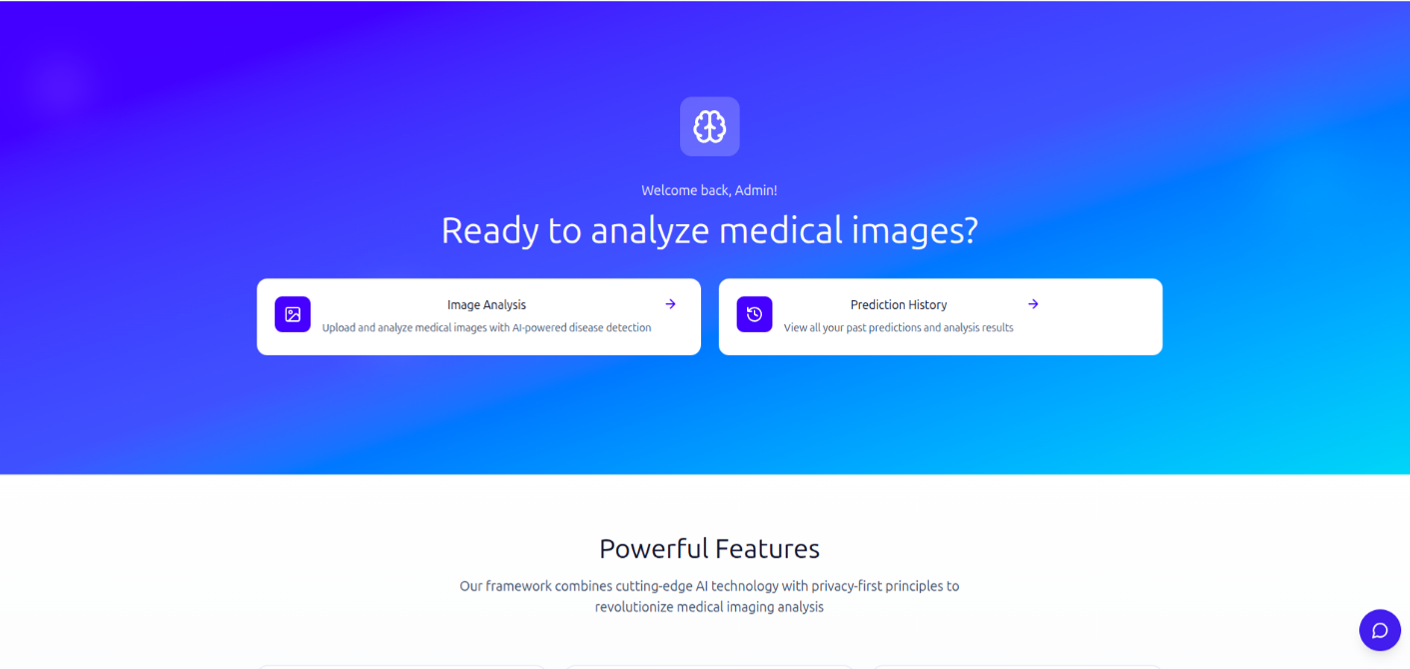
\includegraphics[width=0.95\linewidth]{assets/backend10.png}
	\caption{An image greeting page of the web application.}
	\label{fig:greeting_1}
\end{figure}

\begin{figure}[htbp]
	\centering
	
\includegraphics[width=0.95\linewidth]{assets/backend11.png}
	\caption{An image of the system asking the user to upload a scan to diagnose.}
	\label{fig:greeting_2}
\end{figure}

Prediction history can be viewed and also has statistics like (total scans , AVG. confidence) , and also every prediction’s details can be viewed or deleted, as shown in Figure~\ref{fig:pred_history}, and the details of each scan can be reviewed as well, as shown in Figure~\ref{fig:pred_review}.

\begin{figure}[htbp]
	\centering
	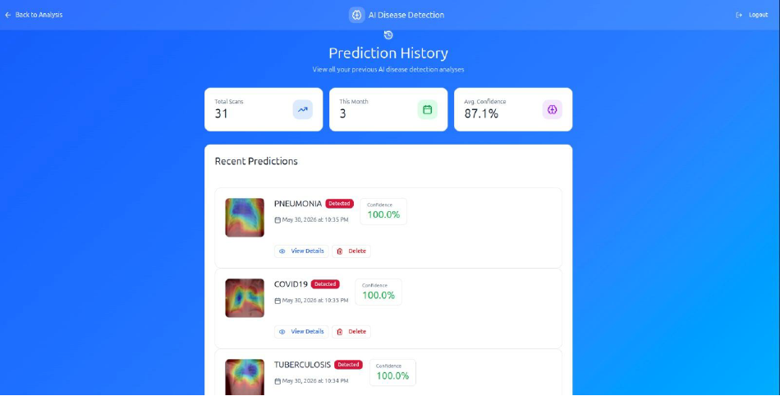
\includegraphics[width=0.95\linewidth]{assets/backend12.png}
	\caption{An image of the system showing the prediction history of the logged-in  user.}
	\label{fig:pred_history}
\end{figure}

\begin{figure}[htbp]
	\centering
	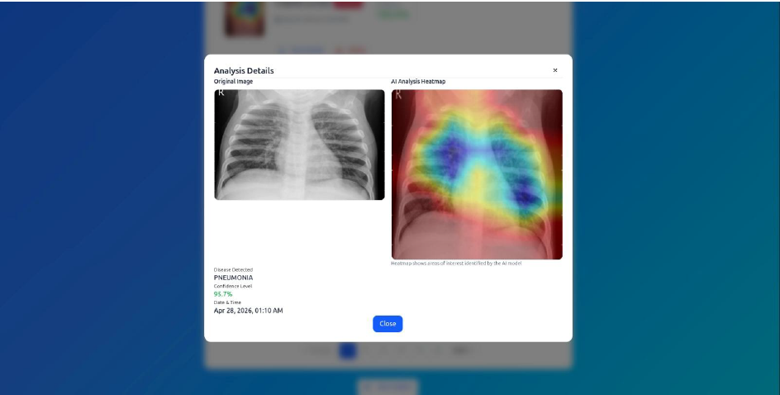
\includegraphics[width=0.95\linewidth]{assets/backend13.png}
	\caption{An image of the system showing the details of one of the user's historical predictions.}
	\label{fig:pred_review}
\end{figure}

Some examples of the Lung Cancer model in action are shown in Figure~\ref{fig:lung1}, and Figure~\ref{fig:lung2}. The system also makes sure to show the confidence as ordinary in medical applications of computer vision systems, as well as the processing time and the resulting heatmap, if applicable.

\begin{figure}[htbp]
	\centering
	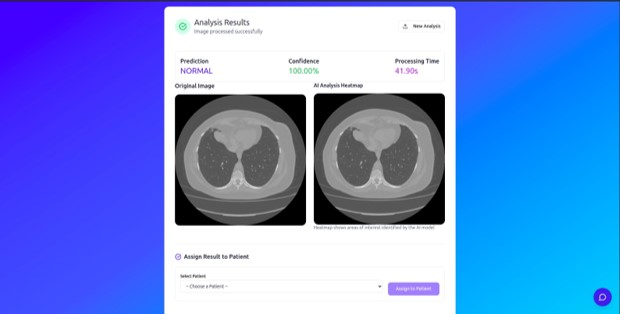
\includegraphics[width=0.95\linewidth]{assets/backend14.jpg}
	\caption{One of the of the examples of using the system on the a lung cancer image.}
	\label{fig:lung1}
\end{figure}

\begin{figure}[htbp]
	\centering
	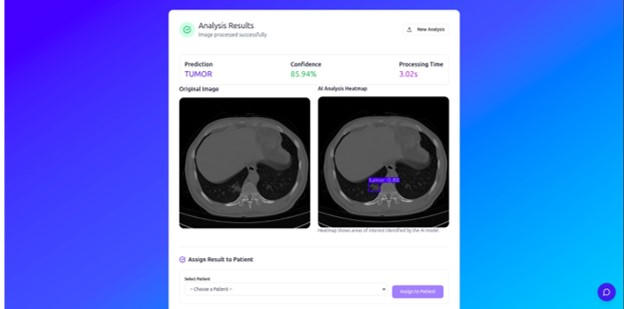
\includegraphics[width=0.95\linewidth]{assets/backend15.jpg}
	\caption{Another example of using the system on the a lung cancer image.}
	\label{fig:lung2}
\end{figure}

\subsubsection{Appointment Management}
The appointment management module enables patients and doctors to coordinate medical consultations through a structured workflow. Patients can create appointments by selecting a doctor, choosing a date and time, specifying the appointment type, and providing optional notes or supporting attachments. Once submitted, the appointment information is stored in the database and becomes available to the assigned doctor.

Doctors can view their scheduled appointments, review patient details, and update the appointment status as needed. They can mark appointments as completed, add consultation notes, or cancel appointments when necessary. Patients can also view the status of their appointments and track any updates made by the doctor.

All appointment data is managed through the Spring Boot backend and stored in PostgreSQL, ensuring persistence and secure access. The module provides an organized way to manage patient-doctor interactions while maintaining a complete record of appointment history within the platform.

\begin{figure}[htbp]
	\centering
	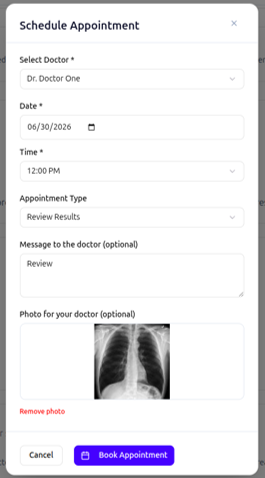
\includegraphics{assets/backend16.png}
	\caption{An image of the Schedule Appointment interaction from the system.}
	\label{fig:appointment_mgmt}
\end{figure}

\paragraph{Real-Time WebSocket}
Spring WebSocket with STOMP over SockJS provides live FL hospital status to the frontend. A scheduled poller runs every 10 seconds, fetches client status from the FL Server, syncs to PostgreSQL, and broadcasts to /topic/fl/clients. Hospital nodes that miss heartbeats are marked OFFLINE automatically.

\paragraph{Email Service}
Spring Mail with Gmail SMTP sends three types of emails:
\begin{itemize}
	\item Password Reset: link to \texttt{/reset-password?token=...}
	\item Admin Invite: link to \texttt{/set-password?token=...} for new doctor/admin accounts
	\item FL hospital onboarding: download link for the hospital Docker client package plus connection details.
\end{itemize}

\paragraph{Core API Modules}
The core modules exposed by the API and implemented in it a re listed in Table~\ref{tab:backend_modules}
\begin{table}[htbp]
	\centering
	\caption{Backend service modules and their responsibilities within the system.}
	\label{tab:backend_modules}
	\begin{tabular}{|p{4cm}|p{9cm}|}
		\hline
		\textbf{Module} & \textbf{Description} \\
		\hline
		
		Authentication &
		Handles the full authentication lifecycle including user registration, login, token issuance, refresh token management, and logout operations. \\
		\hline
		
		Image Upload &
		Generates and returns Cloudflare R2 presigned PUT URLs to enable secure direct client-side uploads of medical images. \\
		\hline
		
		Image Processing &
		Orchestrates the machine learning inference pipeline, triggers model execution, and stores as well as retrieves diagnostic results from the persistence layer. \\
		\hline
		
		Appointments &
		Manages the full appointment workflow, allowing patients to book appointments and doctors to approve, complete, or cancel scheduled sessions. \\
		\hline
		
		Admin User Management &
		Provides administrative capabilities for managing user accounts, including creation, modification, role assignment, and deactivation. \\
		\hline
		
		Federated Learning Hospitals &
		Handles hospital registration and management within the federated learning ecosystem, acting as a proxy interface to the federated learning server. \\
		\hline
		
		Federated Learning Webhooks &
		Processes callback events from the federated learning server after training rounds, updating system state and storing training metadata accordingly. \\
		\hline
		
	\end{tabular}
\end{table}

\subsection{ML Service - ModelBackend}
ModelBackend is a FastAPI microservice that hosts all AI capabilities. At startup it loads four ML components into memory and exposes a unified image-processing endpoint plus a RAG chatbot. It runs on port 8000 and is called by centralized Backend for image analysis and directly by the frontend for chatbot interactions.

\subsubsection{ML Models}
Different backbone models were used for the different tasks the proposed system performs. All the AI models and architectures used are listed in Table~\ref{tab:ml_components}.

\begin{table}[htbp]
	\centering
	\caption{Machine learning components and their corresponding frameworks and purposes within the proposed system.}
	\label{tab:ml_components}
	\begin{tabular}{|p{4cm}|p{5cm}|p{6cm}|}
		\hline
		\textbf{Component} & \textbf{Framework} & \textbf{Purpose} \\
		\hline
		
		Router Model &
		Keras (DenseNet121) &
		Classifies input images into X-ray, CT scan, or out-of-distribution categories using 224×224 image resolution as the first stage of the diagnostic pipeline. \\
		\hline
		
		Chest Classification &
		TensorFlow/Keras (DenseNet121) &
		Performs four-class chest X-ray diagnosis including COVID-19, Normal, Pneumonia, and Tuberculosis classification in a multi-label-ready setup. \\
		\hline
		
		Lung Segmentation &
		TensorFlow/Keras (U-Net) &
		Extracts lung regions from medical images prior to classification to enhance focus on relevant anatomical structures and improve diagnostic accuracy. \\
		\hline
		
		Lung Cancer Detection &
		YOLOv8 &
		Detects and localizes lung cancer regions in CT scans using bounding box predictions for object-level medical diagnosis. \\
		\hline
		
		RAG Stack &
		LangChain, Ollama, and FAISS &
		Implements a retrieval-augmented generation chatbot for medical question answering using vector-based document retrieval and local LLM inference. \\
		\hline
		
	\end{tabular}
\end{table}

FastAPI serves as the AI engine of XFed NeuroScan and relies on Spring Boot to integrate its models into the complete healthcare platform. While FastAPI is responsible for running AI models and generating predictions, Spring Boot manages the workflow and communicates with the AI service whenever analysis is requested.

Separating Spring Boot and FastAPI into two services improves scalability and maintainability, allowing the healthcare system and AI models to be developed, updated, and deployed independently without affecting each other.

\subsubsection{Image Processing Pipeline}
The image processing module is designed to automatically analyze uploaded medical images and route them to the appropriate AI model based on their content. This architecture allows the system to support multiple diagnostic pipelines while maintaining a single entry point for image analysis.

\paragraph{Unified Routing}
Every uploaded image first passes through the Router Model, which serves as the initial classification layer. The router determines whether the image is a chest X-ray, lung cancer image, or an unsupported image type. A confidence threshold of 0.5 is used to ensure reliable routing decisions. Images classified as other are immediately rejected to prevent invalid data from being processed by diagnostic models. Once classified, chest X-rays are forwarded to the DenseNet-based chest disease pipeline, while lung cancer images are sent to the YOLOv8 detection pipeline.

\paragraph{Chest Pipeline}
The chest disease analysis pipeline is optimized for detecting four classes: COVID-19, Pneumonia, Tuberculosis, and Normal. Before classification, several preprocessing steps are applied to improve image quality and model performance.

First, a U-Net lung segmentation model isolates the lung region from the surrounding anatomy, allowing the classifier to focus only on clinically relevant areas. Next, Contrast Limited Adaptive Histogram Equalization (CLAHE) enhances local contrast within the segmented lungs, making subtle abnormalities easier to detect. A Gaussian Blur (5×5) filter is then applied to reduce image noise while preserving important structures.

The processed image is normalized to the range [0,1], converted to RGB format, and resized to 224×224 pixels, which matches the input requirements of the DenseNet model. The DenseNet classifier then predicts one of the four disease categories and returns a confidence score indicating prediction certainty.

To improve explainability, the system generates a Grad-CAM heatmap from the final convolutional layers of the network. This heatmap highlights the image regions that most influenced the model’s decision, providing visual evidence to support the prediction. Both the original image and the generated heatmap are uploaded to Cloudflare R2 for storage and later retrieval by the frontend.

\paragraph{Lung Cancer Pipeline}
The lung cancer pipeline is based on YOLOv8, an object detection model capable of identifying suspicious cancerous regions within medical images. After the router classifies an image as a lung cancer case, it is forwarded directly to the YOLOv8 model for inference.

The model performs real-time detection using a confidence threshold of 0.3, identifying potential cancer regions and generating bounding boxes around detected abnormalities. For each detected region, the model provides confidence scores indicating the likelihood of cancer presence.

The detected regions are then visually annotated on the image by drawing bounding boxes and labels, creating an interpretable result that can be reviewed by medical professionals. The final annotated image is uploaded to Cloudflare R2 under the lung cancer results directory, allowing it to be displayed in the frontend and stored as part of the patient's analysis history.

This dual-pipeline architecture combines classification-based diagnosis for chest diseases with object-detection-based localization for lung cancer, enabling the platform to provide both diagnostic predictions and visual explanations while maintaining a unified processing workflow.

An overall visualization of the image processing pipeline is shown in Figure~\ref{fig:backend_overall}

\begin{figure}[htbp]
	\centering
	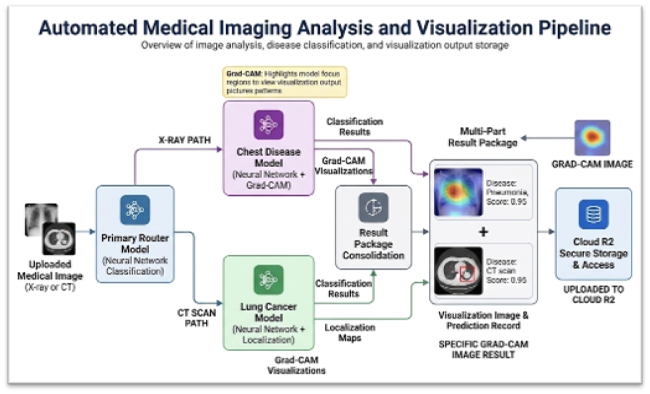
\includegraphics[width=0.95\linewidth]{assets/backend17.png}
	\caption{A simple visualization of the overall image processing pipeline from the backend's perspective.}
	\label{fig:backend_overall}
\end{figure}

\subsubsection{Grad-CAM Explainability and Localization}
For every chest X-ray prediction, the system generates a Grad-CAM (Gradient-weighted Class Activation Mapping) heatmap to provide interpretability for the AI decision. This mechanism highlights the regions of the image that most influenced the model’s prediction by tracing gradients flowing into the final convolutional layers of the DenseNet network.

The generated heatmap is visualized using a JET colormap and overlaid on the original X-ray image , allowing both the anatomical structure and the activated regions to remain clearly visible. This overlay helps radiologists and clinicians visually verify whether the model is focusing on medically relevant areas such as lung opacities, consolidations, or abnormal tissue patterns rather than irrelevant regions.

To support persistence and later retrieval, both the original Grad-CAM output and the processed overlay image are stored in Cloudflare R2 under the \texttt{heatmaps/} directory. These images are served to the frontend using secure presigned URLs, ensuring controlled and time-limited access to sensitive medical data.

\subsubsection{Localization Capability}Beyond explainability, Grad-CAM also provides a form of weak localization for disease regions within the chest X-ray. Although the DenseNet model is primarily designed for classification, Grad-CAM transforms it into a pseudo-localization system by identifying spatial regions that contribute most strongly to the predicted class.

This allows the system to:
\begin{itemize}
	\item Approximate the location of abnormal lung regions.
	\item Highlight areas associated with diseases.
	\item Provide spatial context without requiring a dedicated detection model   
\end{itemize}

In practice, this means the system not only predicts the presence of a disease but also indicates where in the lungs the abnormality is likely located. This improves clinical trust and makes the AI output more interpretable, bridging the gap between pure classification models and spatially aware diagnostic tools.

Overall, Grad-CAM serves as both an explainability mechanism and a lightweight localization method, enhancing transparency and clinical usability of the AI predictions.

\subsubsection{RAG Chatbot Module}
Retrieval-Augmented Generation (RAG) is an AI technique that enhances LLM responses by grounding them in a private document corpus rather than relying solely on the model's pre-trained knowledge. This is critical for domain-specific applications — such as medical systems,  where accuracy, traceability, and up-to-date information are essential.

\paragraph{Standard RAG Pipeline}
\begin{itemize}
	\item Ingest:  Load source documents (PDF, TXT, etc.)
	\item Chunk: Split long documents into overlapping smaller pieces.
	\item Embed: Convert each chunk to a dense numerical vector using a sentence embedding model.
	\item Store: Persist vectors in a FAISS vector database, organized by category.
	\item Retrieve: On a user query, embed the question and find the top-k most similar chunks.
	\item Generate: Pass the retrieved chunks and the question to the LLM to produce a grounded answer.
\end{itemize}

The classifier is the key differentiator of this RAG system. Rather than searching all documents indiscriminately, each query is first categorized, enabling targeted retrieval from the correct FAISS index.

\paragraph{Categories}
\begin{table}[htbp]
	\centering
	\caption{Categories of input handled by the RAG-based medical chatbot.}
	\label{tab:rag_input_categories}
	\begin{tabular}{|p{4cm}|p{9cm}|}
		\hline
		\textbf{Category} & \textbf{Typical Content} \\
		\hline
		
		Medical &
		Queries related to chest diseases and lung cancer, including symptoms, diagnosis, interpretation of medical findings, and general medical imaging questions. \\
		\hline
		
		General &
		Greetings, small talk, and off-topic or non-medical conversational queries that do not require clinical or diagnostic knowledge. \\
		\hline
		
	\end{tabular}
\end{table}

\paragraph{Model Architecture}
The classifier uses a lightweight 1D Convolutional Neural Network (CNN) designed for speed and bilingual text support, the full visualization of the architecture is shown in Figure~\ref{fig:rag_arch}.
\begin{enumerate}
	\item Input: Token IDs (max 50 tokens)
	\item Embedding Layer (vocab $\rightarrow$ 64 dims)
	\item Conv1d (64 $\rightarrow$ 128 channels) + ReLU + Dropout(0.3)
	\item Conv1d (128 $\rightarrow$ 128 channels) + ReLU
	\item AdaptiveMaxPool1d(1)
	\item Fully Connected: 128 $\rightarrow$ 64 $\rightarrow$ 3
	\item Output.
\end{enumerate}

\begin{figure}[htbp]
	\centering
	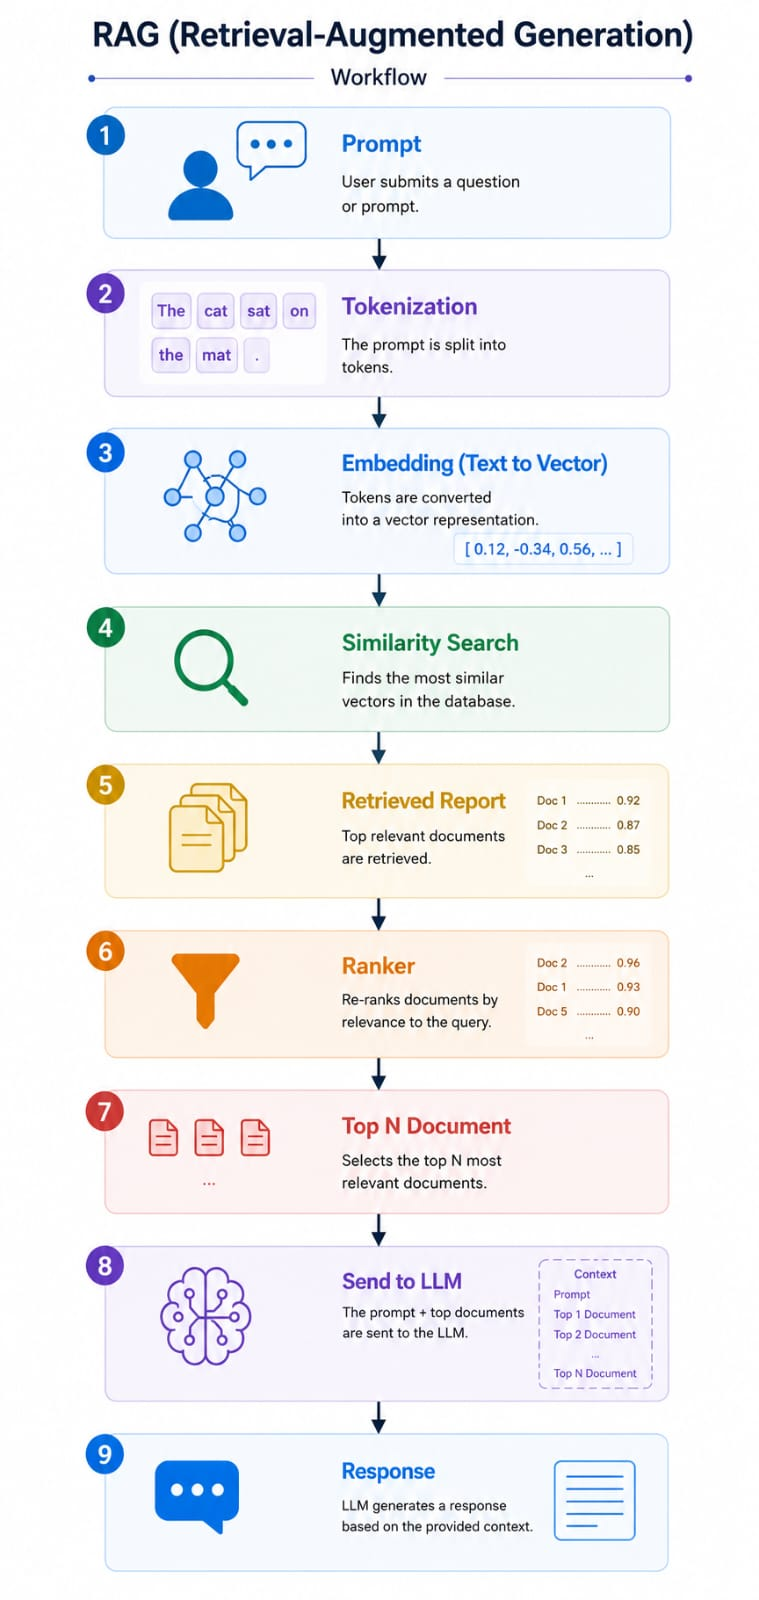
\includegraphics[height=0.90\textheight, keepaspectratio]{assets/backend18.jpeg}
	\caption{A simple visualization of the overall RAG architecture.}
	\label{fig:rag_arch}
\end{figure}

\paragraph{Bilingual Tokenizer}
\begin{itemize}
	\item Tokenizes Arabic , English, and numeric tokens
	\item Vocabulary built from training data (~300+ labeled question pairs)
	\item Fixed-length encoding: max 50 tokens, padded with <PAD>, unknown words as <UNK>
	\item Outputs: classifier.pth, tokenizer.json, config.json
\end{itemize}

\paragraph{Training Configuration}
The model was trained for 100 epochs using the Adam optimizer with a learning rate of 0.001 and a batch size of 16. The vocabulary size is 352 tokens, and each input token is mapped into a 64-dimensional embedding space. The hidden layer dimension is set to 128, Each input sequence is limited to a maximum length of 50 tokens to ensure consistent processing and performance.

\paragraph{LLM Configuration}
The configurations used for the RAG engine are shown in Table~\ref{tab:llm_parameters} for reproduce-ability purposes.
\begin{table}[htbp]
	\centering
	\caption{Configuration parameters of the RAG-based LLM engine.}
	\label{tab:llm_parameters}
	\begin{tabular}{|p{5cm}|p{8cm}|}
		\hline
		\textbf{Parameter} & \textbf{Standalone Value} \\
		\hline
		
		LLM Engine &
		Ollama \\
		\hline
		
		Model &
		qwen2.5:3b \\
		\hline
		
		Temperature &
		0.5 \\
		\hline
		
		Max Tokens &
		500 \\
		\hline
		
		Keep Alive &
		Infinite (-1) \\
		\hline
		
	\end{tabular}
\end{table}

\paragraph{Prompt Design}
The LLM is strictly instructed to answer only from the retrieved context. If the context does not contain the answer, the model is instructed to say "I don't know." Responses are capped at three sentences and must match the language of the question.

The text is split using a RecursiveCharacterTextSplitter with a chunk size of 1000 characters and an overlap of 150 characters between consecutive chunks. This ensures that the text is broken into manageable segments while preserving context between adjacent chunks for better retrieval accuracy.

RAG Independence from Image models  RAG does not receive chest X-ray predictions, GradCAM heatmaps, lung cancer results, or Spring Boot patient records. It is a standalone medical Q\&A chatbot co-located in every page  purely for deployment convenience.

Examples of using the RAG agent implemented in the system are shown in Figure~\ref{fig:rag_examples}

\begin{figure}[htbp]
	\centering
	
	% ---------------- Left Example ----------------
	\begin{subfigure}[t]{0.48\textwidth}
		\centering
		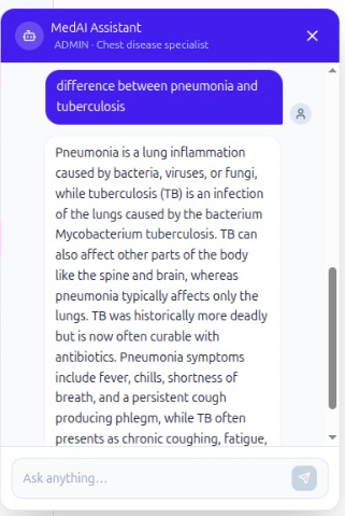
\includegraphics[width=\linewidth]{assets/backend19.png}
		\caption{Example of a medical query processed by the RAG agent, showing retrieval of relevant documents and generated response.}
		\label{fig:rag_example_1}
	\end{subfigure}
	\hfill
	% ---------------- Right Example ----------------
	\begin{subfigure}[t]{0.48\textwidth}
		\centering
		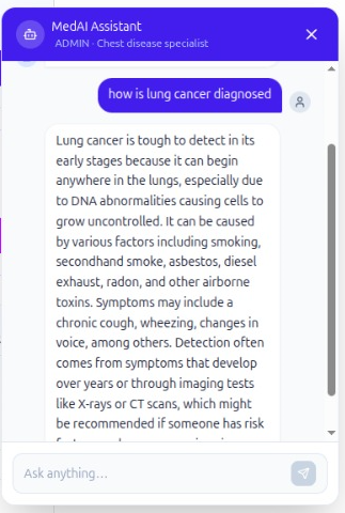
\includegraphics[width=\linewidth]{assets/backend20.png}
		\caption{Example of a general/off-topic query handled by the RAG agent with a conversational response without medical retrieval.}
		\label{fig:rag_example_2}
	\end{subfigure}
	
	\caption{Illustrative examples of the behavior of the retrieval-augmented generation (RAG) agent in different query scenarios. The system adapts its response strategy depending on whether the input is medical or general in nature.}
	\label{fig:rag_examples}
\end{figure}


\subsubsection{Performance Profile}
The performance profile of the proposed system is discussed in Table~\ref{tab:performance_overview}.
\begin{table}[htbp]
	\centering
	\caption{Computational performance and execution environment of the proposed system components.}
	\label{tab:performance_overview}
	\begin{tabular}{|p{5cm}|p{4cm}|p{5cm}|}
		\hline
		\textbf{Component} & \textbf{Approximate CPU Time} & \textbf{GPU} \\
		\hline
		
		Router &
		50--100 ms &
		Automatically enabled if CUDA is available \\
		\hline
		
		Chest Pipeline (Segmentation + Prediction + Grad-CAM) &
		1--5 s &
		CUDA auto-enabled \\
		\hline
		
		Lung Cancer YOLO Inference &
		1--5 s &
		CUDA auto-enabled \\
		\hline
		
		R2 Download / Upload &
		Network-dependent &
		N/A \\
		\hline
		
	\end{tabular}
\end{table}

Running the ModelBackend requires sufficient computational resources because it hosts multiple AI components simultaneously, including image classification models (DenseNet, YOLO, U-Net), the router model, and the RAG pipeline with embedding models and an LLM (Ollama). For stable performance, a GPU is strongly recommended for accelerating deep learning inference, especially for chest X-ray and lung cancer detection tasks.

In addition, the system requires adequate CPU resources to handle concurrent API requests, image preprocessing, and routing logic, while RAM (at least 4–6 GB minimum, higher recommended) is needed to keep multiple models, FAISS indexes, and embeddings loaded in memory without performance degradation. Overall, a balanced setup with a capable GPU, multi-core CPU, and sufficient RAM ensures smooth and responsive AI processing across all services in the ModelBackend

\subsection{Federated Learning Server}
The Federated-Learning-Server is responsible for enabling privacy-preserving collaborative training across multiple hospitals without requiring any centralization of medical data. It allows hospitals to jointly train a shared model while ensuring that raw patient images never leave their local environments, maintaining strict data privacy and compliance with healthcare constraints.

The system is built using a hybrid architecture that combines a FastAPI REST service and a Flower-based gRPC server within a single Python process. The FastAPI layer acts as the control interface for registration, monitoring, and coordination tasks, while the Flower server handles the actual federated learning workflow, including distributed training and weight aggregation.

Both components are synchronized through an in-memory SharedState singleton, which maintains the current training status, active clients, and round coordination signals. This design allows seamless communication between REST-based administrative actions and gRPC-based training execution, ensuring that federated learning rounds are executed in a coordinated and efficient manner across all participating hospitals.

\subsubsection{Design Principles}
The design principles of the federated learning server are listed in Table~\ref{tab:fl_principles}.
\begin{table}[htbp]
	\centering
	\caption{Core design principles and their implementation in the federated learning framework.}
	\label{tab:fl_principles}
	\begin{tabular}{|p{4cm}|p{9cm}|}
		\hline
		\textbf{Principle} & \textbf{Implementation} \\
		\hline
		
		Privacy first &
		Only model weight updates are transmitted between clients and the server; raw medical images never leave the hospital premises under any circumstance. \\
		\hline
		
		On-demand training &
		The Flower server remains idle until explicitly triggered by an administrator via the \texttt{POST /start-round} endpoint, ensuring that training rounds are fully controlled and non-automatic. \\
		\hline
		
		In-process coupling &
		FastAPI and Flower operate within a shared runtime environment using a \texttt{SharedState} singleton, eliminating the need for internal HTTP communication and reducing overhead. \\
		\hline
		
		Weight hot-reload &
		After each federated aggregation round, the updated global model weights are immediately pushed to the Model Backend, enabling real-time deployment of improved models. \\
		\hline
		
	\end{tabular}
\end{table}

The Federated-Learning-Server follows a dual-process architecture where two interconnected services run simultaneously within the same system. The main process runs a Uvicorn-based FastAPI server on port 8001, which acts as the REST bridge responsible for hospital registration, client management, monitoring, and handling webhooks from the main backend system. In parallel, a daemon process runs a Flower gRPC server on port 50051, which is responsible for coordinating the actual federated learning workflow, including distributed training and model weight aggregation across participating hospitals.

This separation allows the system to clearly divide responsibilities between control-plane operations (handled by FastAPI) and training-plane execution (handled by Flower). Both processes share a common in-memory SharedState, ensuring synchronization between REST actions and federated learning events while maintaining efficient and real-time coordination.

\subsubsection{Training Round Lifecycle}
A complete federated training round follows these steps:
\begin{itemize}
	\item Step 1: Admin selects online hospitals and initiates a round
	\item Step 2: Spring calls start-round with round id, min clients, deadline minutes
	\item Step 3: FastAPI sets SharedState \texttt{trigger\_event}, unblocking the Flower server thread
	\item Step 4: Hospital clients receive global weights via gRPC, train locally on their data
	\item Step 5: CustomFedAvg aggregates weight updates using the FedAvg algorithm
	\item Step 6: Aggregated weights saved and pushed to ModelBackend
	\item Step 7: Webhook notifies spring of round completion or failure
	\item Step 8: trigger event cleared; Flower waits for the next admin trigger
\end{itemize}

\begin{figure}[htbp]
\centering
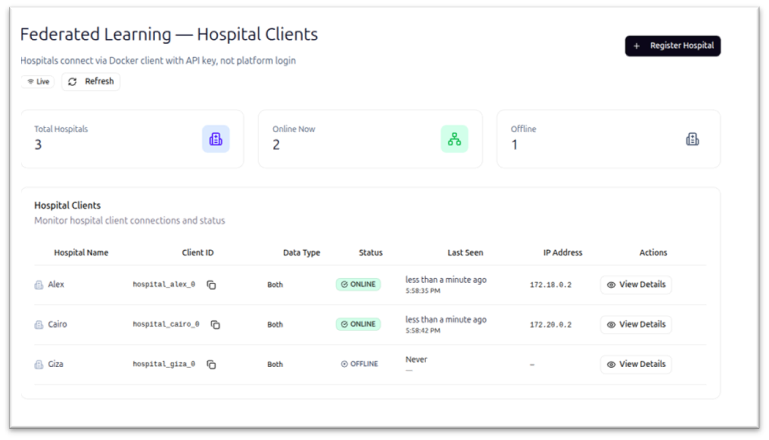
\includegraphics[width=0.95\linewidth]{assets/backend21.png}
\caption{The federated learning dashboard of the web application.}
\label{fig:fed_db}
\end{figure}

After a hospital is successfully registered in the federated learning system, Spring Boot finalizes the onboarding process by generating the necessary FL credentials and preparing a deployment package for that hospital. Once the registration is approved, the system automatically sends an email notification to the hospital using Gmail SMTP.

This email contains all essential onboarding information, including the hospital’s federated learning client ID, encrypted API key, and instructions for connecting to the Federated Learning Server. It also provides a Docker-based hospital client package, which is the only component the hospital needs to run locally.

From the hospital side, the setup process is intentionally simple. The hospital team only needs to:
\begin{enumerate}
	\item Put the data in the required folder
	\item Run the container provided in the package 
\end{enumerate}

Once the container is started, the hospital client automatically connects to the Federated Learning Server, begins sending heartbeat signals, and becomes eligible for participation in training rounds. After this step, no further manual integration is required, as all communication and training coordination are handled automatically by the system.

This design ensures a smooth onboarding process where hospitals do not need to manage complex machine learning setups, and can join the federated learning network by simply configuring and running a pre-built container

Once the container is running and sending heartbeat signals, the hospital is marked as ONLINE and becomes eligible to participate in federated training rounds.

\begin{figure}[htbp]
	\centering
	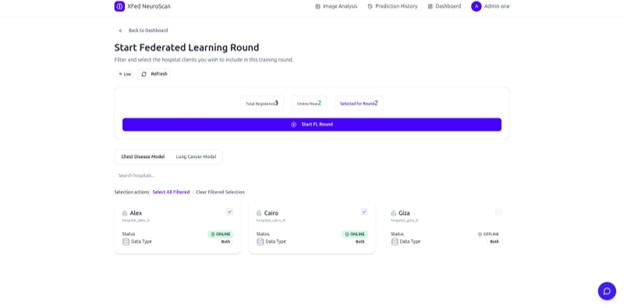
\includegraphics[width=0.95\linewidth]{assets/backend22.jpg}
	\caption{The federated learning management tab.}
	\label{fig:fed_mgmt}
\end{figure}

\subsubsection{Round Status States}
The full states and status code for the federated learning server are listed and explained in Table~\ref{tab:fl_status}
\begin{table}[htbp]
	\centering
	\caption{Federated learning server execution states and their meanings.}
	\label{tab:fl_status}
	\begin{tabular}{|p{3.5cm}|p{10cm}|}
		\hline
		\textbf{Status} & \textbf{Meaning} \\
		\hline
		
		IDLE &
		No federated learning round is currently running; the Flower server is blocked and waiting for an external trigger event. \\
		\hline
		
		STARTED &
		A training round has been triggered and participating hospital clients are actively performing local model training. \\
		\hline
		
		AGGREGATING &
		The server is performing FedAvg aggregation over received client updates to compute the new global model. \\
		\hline
		
		COMPLETED &
		The federated learning round has successfully finished, and the updated global model weights have been saved and pushed to the Model Backend for deployment. \\
		\hline
		
		FAILED &
		The federated learning round has failed due to issues such as timeouts, client-side errors, or model update push failures. \\
		\hline
		
	\end{tabular}
\end{table}

\subsubsection{Security}
The Federated Learning security model is designed to ensure strict isolation between hospitals, the platform backend, and the training infrastructure. A Platform API key is used exclusively by the centralized Backend to securely register new hospital clients, retrieve client lists, and initiate federated learning rounds, ensuring that only the trusted backend can control system-level operations.

Each hospital node is assigned a unique Client API key, which is used solely for heartbeat authentication to confirm that the hospital is online and eligible to participate in training. In addition, a Webhook secret is shared between the FL Server and centralized  Backend to verify and secure all outbound callbacks related to training round completion and status updates.

Hospitals communicate with the system only through outbound connections to port 8001 for REST heartbeats and port 50051 for gRPC-based training, eliminating the need for direct inbound access. Importantly, admin users never interact directly with the FL Server; instead, all operations are securely routed through centralized Backend using JWT authentication, maintaining a centralized and controlled security layer.

The various key types and their roles are shown and explained in great detail in Table~\ref{tab:fl_keys}.

\begin{table}[htbp]
	\centering
	\caption{Authentication key types and their roles within the federated learning system.}
	\label{tab:fl_keys}
	\begin{tabular}{|p{4cm}|p{4.5cm}|p{6cm}|}
		\hline
		\textbf{Key Type} & \textbf{Holder} & \textbf{Scope} \\
		\hline
		
		Platform API Key &
		Centralized Backend &
		Used by the backend system to register clients, initiate federated learning rounds, and retrieve the list of participating clients. \\
		\hline
		
		Client API Key &
		Each hospital node &
		Used exclusively for heartbeat authentication to verify active participation and connectivity of hospital clients. \\
		\hline
		
		Webhook Secret &
		Federated Learning Server and Centralized Backend &
		Used to authenticate outbound callback requests from the federated learning server after training rounds to ensure secure communication. \\
		\hline
		
	\end{tabular}
\end{table}

\subsection{End-to-End Data Flows}
\subsubsection{Medical Image Analysis Flow}
\begin{enumerate}
	\item The frontend user selects an image and requests a presigned URL from the Spring Backend.
	
	\item The frontend uploads the image directly to Cloudflare R2 using the provided presigned URL.
	
	\item After upload, the frontend calls the image processing service with the stored R2 key.
	
	\item The Spring Backend saves image metadata in PostgreSQL, generates a presigned URL, and forwards the request to the FastAPI service via Feign client communication.
	
	\item The FastAPI service downloads the image from R2, routes it using the trained routing model, and executes the appropriate specialist pipeline (either chest disease classification or lung cancer detection).
	
	\item The FastAPI service uploads the generated outputs (such as Grad-CAM heatmaps or annotated detection images) back to R2 and returns the prediction, confidence score, and storage key.
	
	\item The Spring Backend stores the final inference results in the database and generates presigned URLs for secure result visualization.
	
	\item The frontend displays the prediction results, confidence scores, and visual explanations such as Grad-CAM overlays or bounding box annotations to the user.
\end{enumerate}

\subsubsection{User Authentication Flow}
\begin{enumerate}
	\item The user logs in via the login page, where credentials are verified by Spring Security.
	
	\item If authentication succeeds, an access JWT is returned in the response body, and a refresh token is set as an HttpOnly cookie.
	
	\item The refresh token is also stored in Redis with a defined key and a 30-day expiration period.
	
	\item The frontend stores the access token in memory, while the authentication context initializes and loads the user role and profile information.
	
	\item When the access token expires, the frontend calls the refresh token endpoint, which issues a new access token and rotates the refresh cookie.
	
	\item During logout, the access token is blacklisted and the refresh token is removed from Redis, fully invalidating the user session.
\end{enumerate}

\subsubsection{Federated Learning Hospital Status Flow}
\begin{enumerate}
	\item The administrator registers a hospital through the frontend interface, and the Spring forwards the registration request to the Federated Learning (FL) Server.
	
	\item The FL Server generates a unique API key, which is encrypted and stored by the backend. Subsequently, an onboarding email containing the Docker-based client package is sent to the hospital.
	
	\item The hospital deploys the provided Docker client, which establishes a connection to the Flower server via gRPC for federated learning participation.
	
	\item The hospital client initiates a heartbeat process that continuously sends periodic signals to the FL Server every 30 seconds to indicate active status.
	
	\item The Spring Backend executes a polling mechanism every 10 seconds to retrieve the latest client status updates from the FL Server.
	
	\item The retrieved client statuses are synchronized with the PostgreSQL database and broadcast in real time using STOMP WebSocket communication.
	
	\item The frontend subscribes to the WebSocket channel and dynamically updates hospital ONLINE/OFFLINE indicators in real time based on received status updates.
\end{enumerate}


\section{Summary}

This chapter presented the proposed end-to-end model for automated detection of chest diseases and bone fractures from medical images. The overall solution architecture was introduced, highlighting the integration of a deep learning–based diagnostic pipeline with supporting backend processes to enable efficient and scalable medical image analysis.

The deep learning pipeline was described in detail, illustrating the sequential flow from image preprocessing and feature extraction to intelligent routing and task-specific inference. Transfer learning was adopted as a core strategy to leverage pre-trained deep neural networks, enabling effective feature representation and improved generalization in the presence of limited labeled medical data.

The chapter also introduced the medical image routing model, which enables dynamic task allocation by directing input images to specialized diagnostic models. This design enhances modularity and allows the system to support multiple medical imaging tasks within a unified framework.

Then, the architecture of the chest disease classification model was discussed in detail. The design was illustrated, and the use of ResNet50 as the main feature extractor was justified. The formulation of the problem and the motivation behind such a model were presented while detailed architectural aspects of the transfer-learning model were omitted to avoid redundancy.

Finally, the bone fracture detection model was presented as a task-specific component of the system, implemented using an unmodified YOLOv8 architecture. The formulation of the fracture detection problem and the motivation for adopting a one-stage object detection approach were discussed, while detailed architectural aspects were referenced to earlier sections to avoid redundancy.

Overall, this chapter established the structural and methodological foundation of the proposed system, providing a clear understanding of its components and design choices. The described models form the basis for the experimental evaluation and performance analysis presented in the subsequent chapter.